\documentclass{article}
\usepackage{nips14submit_e,times}

%\title{Pure Exploration of Combinatorial Bandits}
\title{Combinatorial Pure Exploration of \\ Multi-Armed Bandits}
\author{Shouyuan Chen}
\date{\today}
%%%%%%%%%%%%%%%%%%%%%%%%%%%%%%%%%%%%%%%%%%%%%%%%%%%%%%%%%%%%%

% Change "article" to "report" to get rid of page number on title page
\usepackage{amsmath,amsfonts,amsthm,amssymb}
\usepackage{setspace}
\usepackage{Tabbing}
\usepackage{fancyhdr}
\usepackage{lastpage} 
\usepackage{extramarks}
\usepackage{chngpage}
\usepackage{soul,color}
\usepackage{graphicx,float,wrapfig}
\usepackage{afterpage}
\usepackage{abstract}
\usepackage[colorlinks=true,linkcolor=blue,citecolor=blue]{hyperref}
\usepackage[numbers]{natbib}
\usepackage[noend]{algpseudocode}
\usepackage{algorithm}
\usepackage{xspace}
\usepackage{subcaption}
\usepackage{theoremref}
\usepackage{thmtools}
\usepackage{thm-restate}
\usepackage{cleveref}

%\usepackage{titling}

\newcommand{\compilehidecomments}{false}

% Macro for comments:
\ifthenelse{ \equal{\compilehidecomments}{true} }{%
	\newcommand{\wei}[1]{}
	\newcommand{\tian}[1]{}
	\newcommand{\shouyuan}[1]{}
}{
	\newcommand{\wei}[1]{{\color{blue!50!black}  [\text{Wei:} #1]}}
	\newcommand{\tian}[1]{{\color{brown!60!black} [\text{Tian:} #1]}}
	\newcommand{\shouyuan}[1]{{\color{green!50!black} [\text{Shouyuan:} #1]}}
}




\allowdisplaybreaks
\frenchspacing
%%%%%%%%%%%%%%%%%%%%%%%%%%%%%%%%%%%%%%%%%%%%%%%%%%%%%%%%%%%%%
% Some tools
\newcommand{\junk}[1]{}

%\newtheorem{define}{Definition}
%\newtheorem{example}{Example}
%\newtheorem{lemma}{Lemma}
%\newtheorem{corollary}{Corollary}
%\newtheorem{theorem}{Theorem}

\declaretheorem{theorem}
\declaretheorem{lemma}
\declaretheorem{corollary}
\declaretheorem{define}
\declaretheorem[name=Fact,Refname={Fact,Facts}]{fact}

\declaretheorem{example}
%\declaretheoremstyle[bodyfont=normalfont]{mystyle}
%\declaretheorem[style=mystyle]{example}

%\def\ttdefault{blg}

\newcommand{\Algorithm}{{\small \textsf{CLUCB}}\xspace}
\newcommand{\AlgorithmPAC}{{\small \textsf{CLUCB-PAC}}\xspace}
\newcommand{\AlgorithmBud}{{\small \textsf{CSAR}}\xspace}
\newcommand{\Uniform}{{\small \textsf{UNI}}\xspace}
%\newcommand{\Problem}{{\small \textsf{ExpCMAB}}\xspace}
\newcommand{\Problem}{{CPE}\xspace}
\newcommand{\Rew}{\varphi}
\newcommand{\E}{\mathbb E}

\newcommand{\M}{\mathcal M}
\newcommand{\mmatch}{\mathcal M_{\mathsf{MATCH}}}
\newcommand{\mtop}{\mathcal M_{\mathsf{TOP}m}}
\newcommand{\mbandit}{\mathcal M_{\mathsf{BANDIT}m}}

\newcommand{\diff}{\mathsf{diff}}
\newcommand{\diffvalid}{\prec}
\newcommand{\B}{\mathcal B}
\newcommand{\C}{\mathcal C}
\newcommand{\del}{\backslash}

\newcommand{\RR}{\mathbb R}

%\newcommand{\vec}[1]{\mathbf #1}

\newcommand{\Bopt}{\mathcal B_{\mathsf{opt}}}
\newcommand{\Bmatch}{\mathcal B_{\mathsf{MATCH}}}
\newcommand{\Btop}{\mathcal B_{\mathsf{TOP}m}}
\newcommand{\Bbandit}{\mathcal B_{\mathsf{BANDIT}m}}

\DeclareMathOperator{\supp}{supp}

\DeclareMathOperator{\rank}{width}
\DeclareMathOperator{\rad}{rad}
\DeclareMathOperator{\decomp}{decomp}
\DeclareMathOperator*{\argmax}{arg\,max}
\DeclareMathOperator*{\argmin}{arg\,min}
\DeclareMathOperator{\Oracle}{Oracle}
\DeclareMathOperator{\COracle}{COracle}
\DeclareMathOperator{\Exchange}{Exchange}

\newcommand{\out}{\mathsf{Out}}
\newcommand{\barlog}{\tilde{\log}}

\let\Pr\undefined
\DeclareMathOperator{\Pr}{Pr}

\newcommand{\MultiIdent}{\textsc{TopK}\xspace}
\newcommand{\MultiBandit}{\textsc{MB}\xspace}
\newcommand{\Matroid}{\textsc{Matroid}\xspace}
\newcommand{\Match}{\textsc{Match}\xspace}
\newcommand{\Path}{\textsc{Path}\xspace}

\newcommand{\inn}[1]{\left\langle #1 \right\rangle}
\newcommand{\nor}[1]{\left\|#1\right\|}
\renewcommand{\vec}[1]{\boldsymbol{#1}}

\renewcommand{\odot}{\circ}

\setlength{\textfloatsep}{1.2em}% Remove \textfloatsep

%%%%%%%%%%%%%%%%%%%%%%%%%%%%%%%%%%%%%%%%%%%%%%%%%%%%%%%%%%%%%

\begin{document}
\newpage

\maketitle
\vspace{-1em}
\begin{abstract}
We study {\em combinatorial pure exploration (\Problem)} problem in the stochastic multi-armed bandit setting,
	where a learner explores a set of arms with the objective of identifying the optimal set of arms
	with certain combinatorial structures, such as size-$K$ subsets, matchings, spanning trees,
	paths, etc.
A collection of subsets of arms with certain combinatorial structure is referred to as a {\em decision class}.	
Instead of solving each \Problem task in an ad-hoc way, we provide a general framework
	as well as solutions that work for all decision classes which admit offline maximization oracles.  
In particular, we present two algorithms for the general \Problem task: 
	one for the fixed confidence setting and one for the fixed budget setting.
We prove problem-dependent upper bounds of our algorithms. 
Our analysis exploits the combinatorial structures of the decision classes and introduces a new analytic tool.
We also establish a general problem-dependent lower bound for the \Problem problem.
Our results show that the proposed algorithms achieve optimal sample complexity (within logarithmic factors) for many decision classes. 
In addition, applying our results back to problems of top-$K$ arms identification and multiple bandit best arms identification, we recover the state-of-the-art upper bounds and settles two open conjectures on the lower bounds.

%\wei{Currently not mentioning PAC result extension. Perhaps OK as long as we mention it in the intro.}

%We study the structured pure exploration problem in the stochastic multi-armed bandit setting.
%In particular, we formulate the \Problem problem where a learner's objective is to identify the optimal set of arms from a collection of sets of arms which we called decision class.
%The decision class could be a collection of size $K$ subsets, matchings, spanning trees or paths. 
%The generality of decision classes allows \Problem to represent a rich class of structured pure exploration problems.
%We present two algorithms for the \Problem problem: one for the fixed confidence setting and one for the fixed budget setting.
%We prove problem-dependent upper bounds of our algorithms. 
%Our analysis exploits the combinatorial structures of the decision classes and introduces a new analytic tool.
%We also establish a general problem-dependent lower bound for the \Problem problem.
%Our results show that the proposed algorithms achieve optimal sample complexity (within logarithmic factors) for many decision classes. 
%In addition, applying our results back to problems of top-$K$ arms identification and multiple bandit best arms identification, we recover the best known upper bounds and settles two open conjectures on the lower bounds.


% objective is to identify the optimal set of arms from a collection of sets of arms called decision class.

\end{abstract}
\vspace{-0.3em}
\section{Introduction}
\vspace{-0.3em}
%After introduced in the seminal work of \citet{robbins1985some}, 
Multi-armed bandit (MAB) is a predominant model for characterizing the tradeoff between exploration and exploitation in decision-making problems. 
Although this tradeoff is intrinsic in many tasks, some application domains prefer a dedicated exploration procedure in which the goal is to identify an optimal object among a collection of candidates and the reward or loss incurred during exploration is irrelevant.
In light of these applications, the related learning problem, called pure exploration in MABs, has received much attention.
Recent advances in pure exploration MABs have found potential applications in many domains including crowdsourcing, communication network and online advertising.

In many  of these application domains, a recurring problem is to identify an optimal object with certain \emph{combinatorial structures}. 
For example, a crowdsourcing application may want to find the best assignment from workers to tasks such that overall productivity of workers are maximized. 
A network routing system during the initialization phase may try to build a spanning tree that minimizes the delay of links, or attempts to identify the shortest path between two sites.  
An online advertising system may be interested to find the best matching between ads and display slots. 
The literature of pure exploration MAB problems lacks a framework that encompasses these kinds of problems where the object of interest has a non-trivial combinatorial structure.  
Our paper contributes such a framework which accounts for general combinatorial structures, and develops a series of results, including algorithms, upper bounds and lower bounds for the framework.

In this paper, we formulate the {\em combinatorial pure exploration (\Problem)} problem for stochastic multi-armed bandits.  
In the \Problem problem, a learner has a fixed set of arms and each arm is associated with an unknown reward distribution. 
The learner is also given a collection of sets of arms called \emph{decision class}, which
	corresponds to  certain collection of combinatorial structures.
During the exploration period, in each round the learner chooses an arm to play
	and observes a random reward sampled from the associated distribution. 
The objective is when the exploration period ends, the learner outputs a member of the decision
	class that she believes to be optimal, in the sense that the sum of expected rewards of all arms
	in the output set is maximized among all members in the decision class.


The \Problem framework represents a rich class of pure exploration problems.
The conventional pure exploration problem in MAB, where the objective is to find the single best arm, clearly fits into this framework, in which the decision class is the collection of all singletons. 
This framework also naturally encompasses several recent extensions, including the problem of finding the top $K$ arms (henceforth \MultiIdent) \citep{kalyanakrishnan2010efficient,kalyanakrishnan2012pac,bubeck2013multiple,zhou2014optimal} and the
multi-bandit problem of finding the best arms simultaneously from several disjoint sets of arms (henceforth \MultiBandit) \citep{NIPS2011_4478,bubeck2013multiple}.
% by constructing proper decision classes. 
%The decision classes associated with these problems are relatively flat. 
Furthermore, this framework  covers many more interesting cases where the decision classes correspond to collections of non-trivial combinatorial structures.
%By allowing general decision classes, this framework represents a rich class of pure exploration problems including many interesting cases where the decision classes correspond to non-trivial combinatorial structures.
%More interesting cases 
%Apart from these simple cases, the decision classes may correspond to non-trivial combinatorial structures. 
%Mo a substantially larger class of pure exploration problems.
For example, suppose that the arms represent the edges in a graph.
Then a decision class could be the set of all paths between two vertices, all spanning trees or all matchings of the graph. 
And, in these cases, the objectives of \Problem correspond to identifying the optimal paths, spanning trees and matchings, respectively.
As we have explained earlier, these types of combinatorial pure exploration problems admit potential applications in diverse domains.% including crowdsourcing, network routing and online advertising.
%Therefore, due to its generality, our framework admits applications in diverse domains including the examples we previously explained.

%More importantly, our framework covers a substantially larger class of pure exploration problems including many interesting cases where the decision classes correspond to non-trivial combinatorial structures. 
%For example, suppose that the arms represent the edges in a graph, then a decision class could be the set of all paths between two vertices, all spanning trees or all matchings of the graph. 
%As we have explained, exploring objects with these kind of structures may have applications 
%Therefore, by choosing different decision classes, our framework represents a rich class of pure exploration problems.

%Finding optimal objects from decision classes with non-trivial structures
The \Problem framework raises several interesting challenges to the design and analysis of pure exploration algorithms. 
One challenge is that, instead of solving each type of \Problem task in an ad-hoc way, one requires a unified algorithm and analysis that supports different decision classes.
Another challenge stems from the combinatorial nature of \Problem, namely that the optimal set may contain some arms with very small expected rewards (e.g. a maximal matching may contain the edge with the smallest weight); hence arms with suboptimal rewards cannot be eliminated  during the learning process or be ignored in the analysis. This differs from many existing approach of pure exploration MABs.
%Another challenge stemming from the combinatorial nature of the \Problem problem is that 
%Another challenge is that the arms with the largest mean rewards may not belong to the optimal set. 
%This challenge stems from the combinatorial nature of the \Problem problem.
%For example, consider the case where the decision class is the set of all matchings in a bipartite graph.  
%In this case, a matching consisting of edges with relatively small weights may turn out to be optimal.  
%However, in many existing algorithms for pure exploration MABs, arms would no longer be considered once their expected reward are proven suboptimal during the learning process. 
Therefore, the design and analysis of algorithms for \Problem demands novel techniques which take both rewards and combinatorial structures into account.
\junk{
Before describing our results, we recall two common settings in pure exploration problems: fixed confidence and fixed budget. 
In the fixed confidence setting, the learner need to guarantee that she correctly identifies the optimal set with high probability while uses a small number of rounds(samples).  
In the fixed budget setting, the learner uses at most a fixed number of samples and she need to minimize her probability of error (identifies a suboptimal set).
}

\textbf{Our results.}
In this paper, we propose two novel learning algorithms for general \Problem problem: one for the fixed confidence setting and one for the fixed budget setting.
Both algorithms support a wide range of decision classes in a unified way. 
%In this paper, we develop a learning algorithm for the \Problem problem in the fixed confidence setting that supports a very wide range of decision classes, which is referred as Combinatorial Gap Exploration (\Algorithm) algorithm.%
In the fixed confidence setting, we present Combinatorial Lower-Upper Confidence Bound (\Algorithm) algorithm.
The \Algorithm algorithm does not need to know the definition of the decision class, as long as it has access to the decision class through a maximization oracle.
%Algorithm is an efficient and practical algorithm that works for a very wide range of decision classes. 
We upper bound the number of samples used by \Algorithm. 
This sample complexity bound depends on both expected reward and the structure of decision class. 
Our analysis relies on a novel combinatorial construction called \emph{exchange class} which may be of independent interest for other combinatorial optimization problems. 
When specializing our result into \MultiIdent and \MultiBandit, we recover previous sample complexity bounds \citep{kalyanakrishnan2012pac,gabillon2012best} up to constant factors.
% with a small improvement in the logarithmic factors. 
While for other decision classes in general, our result establishes the first sample complexity upper bound. 
We further show that \Algorithm can be easily extended to the fixed budget setting and PAC learning setting and we provide related theoretical guarantees in the supplementary material.  

Moreover, we establish a problem-dependent sample complexity lower bound for the \Problem problem.  
Our lower bound shows that the sample complexity of the proposed \Algorithm algorithm is optimal (to within logarithmic factors) for a large class of decision classes, including \MultiIdent, \MultiBandit and the decision classes derived from matroids (e.g. spanning tree). 
Therefore our upper and lower bounds  provide a near full characterization of the sample complexity of these \Problem problems. 
For more general decision classes, our results show that the upper and lower bounds are within a relatively benign factor. 
To the best of our knowledge, there are no problem-dependent lower bounds known for pure exploration MABs besides the case of identifying the single best arm \citep{mannor2004sample,audibert2010best}.
We also notice that our result resolves the open conjectures of \citet{kalyanakrishnan2012pac} and \citet{bubeck2013multiple} on the problem-dependent sample complexity lower bounds of \MultiIdent and \MultiBandit problems.

In the fixed budget setting, we present a parameter-free algorithm called Combinatorial Successive Accept Reject (\AlgorithmBud) algorithm.
We prove a probability of error bound of the \AlgorithmBud algorithm. 
This bound can be shown to be equivalent to the sample complexity bound of \Algorithm within logarithmic factors, although the two algorithms are based on quite different techniques. 
Our analysis of \AlgorithmBud re-uses exchange classes as tools. 
This suggests that exchange class may be useful for the analysis of similar problems. 
In addition, when applying the algorithm to back \MultiIdent and \MultiBandit, our bound recovers a recent result due to \citet{bubeck2013multiple}. 

\junk{
\textbf{Useful notations.} Let $[n]$ denote the set $\{1,\ldots,n\}$. Suppose that $\vec w\in \RR^{n}$ is a vector and $E\subseteq[n]$ is a set. 
Let $w(i)$ denote the $i$-th entry of $\vec w$. 
We define $w(E) \triangleq  \sum_{i\in E} w(i)$ to be the sum of entries indexed by $E$.
%Furthermore, we will use the convention that $\max_{M\in \emptyset} f(M) = -\infty$ for any real-valued function $f$. \wei{Do we need this convention?}
}
\vspace{-0.7em}
\section{Problem Formulation}
\vspace{-0.7em}
%Let $\vec u \in \RR^{n}$ be a vector. 
% and $M\subseteq [n]$ be a set. 
%\textbf{\Problem: problem formulation.} 
In this section,  we formally define the \Problem problem.
Suppose that there are $n$ arms and the arms are numbered $1,2,\ldots,n$.
Assume that each arm $e\in[n]$ is associated with a reward distribution $\Rew_e$.
% and we let $w(e)=\E_{X\sim \Rew_e}[X]$ denote the expected reward. 
Let $\vec w = \big(w(1),\ldots, w(n)\big)^T$ denote the vector of expected rewards, where each entry $w(e)=\E_{X\sim \Rew_e}[X]$ denote the expected reward of arm $e$.
Following standard assumptions of stochastic MABs, we assume that all reward distributions have $R$-sub-Gaussian tails for some known constant $R>0$. 
Formally, if $X$ is a random variable drawn according to $\Rew_e$, then, for all $t\in \RR$, one has $\mathbb E\big[\exp(tX-t\mathbb E[X])\big] \le \exp(R^2t^2/2)$ and $\mathbb E\big[\exp(t\mathbb E[X]-tX)\big] \le \exp(R^2t^2/2)$.
It is well-known that the family of $R$-sub-Gaussian tail distributions encompasses all distributions that are supported on $[0,R]$ as well as many unbounded distributions such as Gaussian distributions with variance $R^2$ (cf. \citep{pollard2000asymptopia}).


We define a \emph{decision class} $\M \subseteq 2^{[n]}$ as a   collection of sets of arms.
Let $M_*=\argmax_{M\in \M} w(M)$ denote the optimal set belonging to the decision class $\M$ which maximizes the sum of expected reward\footnote{We denote $v(M)\triangleq \sum_{i\in[n]} v(i)$ for any vector $\vec v\in\RR^{n}$ and any set $M\subseteq[n]$. For convenience, we will assume that $M_*$ is unique.}. 
A learner's objective is to identify $M_*$ from $\M$ by playing the following game with the stochastic environment.
%Let $\M\subseteq 2^{[n]}$ be the family of all feasible solutions to a combinatorial problem.
%Let $M_* = \argmax_{M\in \M} w(M)$ denote the optimal set of arms which max
%A learner wants to find the optimal solution of $\M$ which maximizes the expected reward $M_*=\argmax_{M\in \M} w(M)$ by playing the following game.
%The learning problem of pure exploration combinatorial bandit can be formalized as a game between a learner and a stochastic environment, where the learner's goal is to find the optimal solution to the combinatorial problem which maximizes the sum of expected reward $M_* = \argmax_{M\in \M} w(M)$.v
At the beginning of the game, the decision class $\M$ is revealed to the learner while the reward distributions $\{\Rew_e\}_{e\in[n]}$ are unknown to the learner.
Then, the learner plays the game over a sequence of rounds;
in each round $t$, the learner pulls an arm $p_t\in [n]$ and observes a reward sampled from the associated reward distribution $\Rew_{p_t}$.
The game continues until certain stopping condition is satisfied.
%which will be specified later.
After the game finishes, the learner need to output a set $\out \in \M$.
%For the sake of simplicity, we shall assume that the optimal set $M_*$ is unique throughout the paper.

%Let $n$ denote the number of arms and suppose that the arms are numbered $1,2,\ldots,n$.

%We assume that all reward distributions are $R$-sub-Gaussian [].
%Notice that all distributions that are supported on $[0,R]$ are $R$-sub-Gaussian distributions [] and therefore our model subsumes the cases of bounded rewards.
%Let $w(e)=\E_{X\sim \Rew_e}[X]$ denote the expected reward of arm $e$ and let $\vec w = \big(w(1),\ldots,w(n)\big)^T$ denote the vector of expected rewards.
%In addition, for any set of arms $M\subseteq [n]$, we define $w(M) = \sum_{e\in M} w(e)$ as the sum of expected rewards of arms that belong to $M$.

%Notice that, if $\epsilon = 0$, then the learner is required to identify the optimal set, i.e. $\out = M_*$.



%\textbf{Fixed confidence and fixed budget.} 
We consider two different stopping conditions of the game, which are known as \emph{fixed confidence} setting and \emph{fixed budget} setting in the literature.
In the fixed confidence setting, the learner can stop the game at any round. 
The learner need to guarantee that $\Pr[\out = M_*] \ge 1-\delta$ for a given confidence parameter $\delta$.
%and her goal is to achieve a fixed confidence about the optimality of the returned set while uses a small number of pulls.
%Specifically, given a confidence parameter $\delta$, the learner 
The learner's performance is evaluated by her \emph{sample complexity}, i.e. the number of pulls used by the learner.
%Notice that the learner can stop the game at any point in this setting.
In the fixed budget setting, the game stops after a fixed number $T$ of rounds, where $T$ is given before the game.
The learner tries to minimize the \emph{probability of error}, which is formally $\Pr[\out \not= M_*]$, within $T$ rounds.
In this case, the learner's performance is measured by the probability of error.

%The generality of \Problem framework stems from the allowance of arbitrary decision classes $\M$.
%Two of the aboves examples, \MultiIdent and \MultiBandit, are studied 


%Finally, for the sake of simplicity, we will assume that the optimal solution $M_*$ is unique.

%\textbf{Useful notations.}
%For any vector $\vec v\in \RR^n$ and any set $M \subseteq [n]$, we define $v(M) = \sum_{e\in M} v(e)$.

\vspace{-0.7em}
\section{Algorithm, Exchange Class and Sample Complexity}
\vspace{-0.7em}
%Our main contribution is an algorithm for solving the \Problem problem.
%Our algorithm 

%In this section, we describe our algorithm for pure exploration combinatorial bandit problem.
%Then, we analyze the sample complexity and the probability of error of our algorithm.

In this section, we present Combinatorial Lower-Upper Confidence Bound (\Algorithm) algorithm, a learning algorithm for the \Problem problem in the fixed confidence setting, and analyze its sample complexity. 
En route to our sample complexity bound, we introduce the notions of exchange class and the widths of decision classes.
% which characterize certain exchange properties of combinatorial structures.
%Our analysis uses tools developed using exchange classes.
%Then, we analyze the sample complexity of \Algorithm algorithm.
Furthermore, the \Algorithm algorithm can be extended to the fixed budget and PAC learning settings,
	the discussion of which is included in the supplementary material (Section~\ref{section:extensions}).
%Now we begin with introducing the notion of oracles.
%Many common combinatorial problems admit computationally efficient oracles.

\textbf{Oracle.}
We allow the \Algorithm algorithm to access a \emph{maximization oracle}. 
A maximization oracle takes a weight vector $\vec v \in \RR^{n}$ as input and finds an optimal set from a given decision class $\M$ with respect to the weight vector $\vec v$.
Formally, we call a function $\text{Oracle:}~\RR^{n} \rightarrow \M$ a maximization oracle for $\M$ if, for all $\vec v\in \RR^{n}$, we have $\Oracle(\vec v) \in \argmax_{M\in \M} v(M)$.
It is clear that a wide range of decision classes admit such maximization oracles, including decision classes correspond to collections of matchings, paths or bases of matroids (see later for concrete examples).
Besides the access to the oracle, \Algorithm does not need \emph{any} additional knowledge of the decision class $\M$.

%For most non-trivial combinatorial problems, the size of the collection of feasible sets $\M$ is exponential in $n$.
%Hence, the definition of $\M$ 
%Therefore, the learning algorithm needs a succinct representation of $\M$.
%In particular, we allow the learning algorithm to use a \emph{maximization oracle} which can find the optimal set $M\in \M$ when the expected reward of each arm is known.
%Specifically, we assume that there exists an oracle which takes a vector $\vec v = \big(v(1),\ldots,v(n)\big)^T$ as input and returns a set $\Oracle(\vec v) = \argmax_{M\in \M} v(M)$.


\textbf{Algorithm.} 
Now we describe the details of \Algorithm, as shown in Algorithm~\ref{algo:pac}.
%
%Our algorithm works for both fixed confidence and fixed budget settings.
%In either settings, the behaviors of our algorithm only differ in the construction of confidence radius and the stopping condition.
%In the following, we describe the procedure of our algorithm.
During its execution, the \Algorithm algorithm maintains empirical mean $\bar w_t(e)$ and confidence radius $\rad_t(e)$ for each arm $e\in[n]$ and each round $t$.
%\wei{Do we still want to change $\bar w_t(e)$ to $\hat w_t(e)$?}
The construction of confidence radius ensures that $|w(e)-\bar w_t(e)| \le \rad_t(e)$ holds with high probability for each arm $e \in [n]$ and each round $t>0$.
\Algorithm begins with an initialization phase in which each arm is pulled once.
Then, at round $t \ge n$, \Algorithm uses the following procedure to choose an arm to play. 
First, \Algorithm calls the oracle which finds the set $M_t=\Oracle(\vec {\bar w}_t)$. 
The set $M_t$ is the ``best'' set with respect to the empirical means $\vec {\bar w}_t$.
% which maximizes empirical means $\bar w_t$ up to  $t$.
Then, \Algorithm explores possible refinements of $M_t$. 
In particular, \Algorithm uses the confidence radius to compute an adjusted expectation vector $\vec {\tilde w}_t$ in the following way: for each arm $e \in M_t$, $\tilde w_t(e)$ equals to the lower confidence bound $\tilde w_t(e) = \bar w_t(e)-\rad_t(e)$; and for each arm $e\not\in M_t$, $\tilde w_t(e)$ equals to the upper confidence bound $\tilde w_t(e)=\bar w_t(e)+\rad_t(e)$.
Intuitively, the adjusted expectation vector $\vec {\tilde w}_t$ penalizes arms belonging to the current set $M_t$ and encourages exploring arms out of $M_t$.
\Algorithm then calls the oracle using the adjusted expectation vector $\vec {\tilde w}_t$ as input to compute a refined set $\tilde M_t = \Oracle(\vec {\tilde w}_t)$.
If $\tilde w_t(\tilde M_t) = \tilde w_t(M_t)$ then \Algorithm stops and returns $\out=M_t$.
%\wei{Is there a difference of using $\tilde w_t(\tilde M_t) = \tilde w_t(M_t)$ or using
Otherwise, \Algorithm pulls the arm belonging to the symmetric difference $(\tilde M_t \del M_t) \cup (M_t \del \tilde M_t)$ between $M_t$ and $\tilde M_t$ which has the largest confidence radius.
This ends the $t$-th round of \Algorithm.
We note that \Algorithm generalizes and unifies the ideas of several different fixed confidence algorithms dedicated to the \MultiIdent and \MultiBandit problems in the literature \citep{kalyanakrishnan2012pac,gabillon2012best,kaufmann2013information}.

\begin{algorithm}[tb]
{
\small
\begin{algorithmic}[1]
\Require Confidence $\delta \in (0,1)$; Maximization oracle: $\Oracle(\cdot): \RR^n \rightarrow \M$
\Statex \textbf{Initialize:} Play each arm $e \in [n]$ once. Initialize empirical means $\vec {\bar w}_n$ and set $T_{n}(e) \gets 1$ for all $e$.
\For{$t=n,n+1,\ldots$}
	\State $M_t \gets \Oracle(\vec {\bar w}_t)$
  \State Compute confidence radius $\rad_{t}(e)$ for all $e\in[n]$
  \Comment{$\rad_t(e)$ is defined later in Theorem~\ref{theorem:main}}
	\For{$e = 1,\ldots,n$}
		\State \textbf{if } $e\in M_t$ \textbf{then } $\tilde w_t(e) \gets \bar w_t(e)-\rad_t(e)$
		\State \textbf{else } $\tilde w_t(e) \gets \bar w_t(e)+\rad_t(e)$
	\EndFor
	\State $\tilde M_t \gets \Oracle(\vec{\tilde w}_t)$
	\If{$\tilde w_t(\tilde M_t) = \tilde w_t(M_t)$}
		\State $\out \gets M_t$
		\State \textbf{return} $\out$
	\EndIf
	\State $p_t \gets \argmax_{e\in (\tilde M_t \del M_t) \cup (M_t \del \tilde M_t)} \rad_t(e)$\label{algo:step:D}
  \Comment{Break ties arbitrarily}
	\State Pull arm $p_t$ and observe the reward
	\State Update empirical means $\vec {\bar w}_{t+1}$ using the observed reward
	\State Update number of pulls: $T_{t+1}(p_t)\gets T_{t}(p_t)+1$ and $T_{t+1}(e) \gets T_{t}(e)$ for all $e\not=p_t$
	\EndFor
\end{algorithmic}
\caption{\Algorithm: Combinatorial Lower-Upper Confidence Bound}
\label{algo:pac}
}
\end{algorithm}

\vspace{-0.5em}
\subsection{Sample complexity}
\vspace{-0.5em}
%In this part, we analyze the performance of Algorithm~\ref{algo:pac} for both fixed confidence and fixed budget settings. 
Now we establish a problem-dependent sample complexity bound of the \Algorithm algorithm. 
%Our sample complexity bound depends on the combinatorial structure of the decision class $\M$. 
To formally state our result, we need to introduce several notions.
%To state our results, we need to define two quantities: gap and width.

\textbf{Gap.} We begin with defining a natural hardness measure of the \Problem problem. 
For each arm $e \in [n]$, we define its gap $\Delta_e$ as
\begin{equation}
\label{eq:define-delta}
\Delta_e = \begin{cases}
			   w(M_*)-\max_{M\in \M: e\in M} w(M) & \text{if } e\not \in M_*, \\
			   w(M_*)-\max_{M\in \M: e\not \in M} w(M) & \text{if } e\in M_*,
			\end{cases}
\end{equation}
where we use the convention that the maximum value of an empty set is $-\infty$. 
%Therefore the gap $\Delta_e$ of a redundant arm $e\not \in M$ for all $M\in \M$ is $+\infty$.
We also define the hardness $\mathbf H$ as the sum of inverse squared gaps 
\begin{equation}
\label{eq:hardness}
\mathbf H =\sum_{e\in [n]} \Delta_e^{-2}.
\end{equation}

From Eq.~\eqref{eq:define-delta}, we see that, for each arm $e\not\in M_*$, the gap $\Delta_e$ represents the sub-optimality of the best set that includes arm $e$; and, for each arm $e\in M_*$, the gap $\Delta_e$ is the sub-optimality of the best set that does not include arm $e$.
This naturally generalizes and unifies previous definitions of gaps \citep{audibert2010best,NIPS2011_4478,kalyanakrishnan2010efficient,bubeck2013multiple}.
%We notice that, for many combinatorial problems, the definition Eq.~\eqref{eq:define-delta} naturally reflects the hardness of an arm.
%().
%Figure X illustrates these interpretations.
%When specializing to \MultiIdent and \MultiBandit, our definition resembles the previous definition of gaps \citep{kalyanakrishnan2012pac,NIPS2011_4478,gabillon2012best,kalyanakrishnan2010efficient,bubeck2013multiple}.



\textbf{Exchange class and the width of a decision class.} 
A notable challenge of our analysis stems from the generality of \Algorithm which, as we have seen, supports a wide range of decision classes $\M$.
Indeed, previous algorithms for special cases including \MultiIdent and \MultiBandit require a separate analysis for each individual type of problem.
Such strategy is intractable for our setting and we need a unified analysis for all decision classes.
Our solution to this challenge is a novel combinatorial construction called \emph{exchange class}, which is used as a proxy for the structure of the decision class.
Intuitively, an exchange class $\B$ for a decision class $\M$ can be seen as a collection of ``patches'' (borrowing concepts from software engineering) such that, for any two different sets $M,M'\in \M$, one can transform $M$ to $M'$ by applying a series of patches of $\B$; and each application of a patch yields a valid member of $\M$.
These patches are later used by our analysis to build gadgets that interpolate between different members of the decision class and serve to bridge key quantities.
Furthermore, the maximum patch size of $\B$ will play an important role in our sample complexity bound.
%Furthermore, we see that the granularity of such interpolation is controlled by the size of patches in $\B$: the smaller patches, the finer granularity.
%Furthermore, if all patches in $\B$ are small (bounded away from $n$), then we are allowed to interpolate with a fine granularity.
%Indeed, the maximum patch size of $\B$ plays an important role in our sample complexity bound.
%In addition, the smaller the patches are the 

%The analysis of our algorithm depends on certain exchange properties of combinatorial structures.
%To capture these properties, we introduce notions of \emph{exchange set} and \emph{exchange class} as tools for our analysis.
%We present their definitions in the following.

%An exchange set is defined as a pair of disjoint sets.
Now we formally define the exchange class.
We begin with the definition of exchange sets, which formalize the aforementioned ``patches''.
We define an exchange set $b$ as an ordered pair of disjoint sets $b=(b_+,b_-)$ where $b_+\cap b_- = \emptyset$ and $b_+,b_-\subseteq [n]$.
Then, we define operator $\oplus$ such that, for any set $M \subseteq [n]$ and any exchange set $b=(b_+,b_-)$, we have $M\oplus b \triangleq M\del b_- \cup b_+$.
Similarly, we also define operator $\ominus$ such that $M\ominus b \triangleq M\del b_+\cup b_-$.

%\wei{There is no intuitive connection on exchange class with the regret bound. Also,
%it would be better to intuitively explain why those exchange sets are patches.}
We call a collection of exchange sets $\B$ an \emph{exchange class for $\M$} if $\B$ satisfies the following property.
For any $M,M'\in \M$ such that $M\not = M'$  and for any $e\in (M\del M')$, there exists an exchange set $(b_+,b_-)\in \B$ which satisfies five constraints: \textbf{(a)} $e\in b_-$, \textbf{(b)} $b_+ \subseteq M'\del M$, \textbf{(c)} $b_- \subseteq M \del M'$, \textbf{(d)} $(M\oplus b) \in \M$ and \textbf{(e)} $(M'\ominus b) \in \M$.

Informally, constraints \textbf{(b)} and \textbf{(c)} resemble the concept of patches in the sense that $b_+$ contains only the ``new'' elements from $M'$ and $b_-$ contains only the ``old'' elements of $M$; constraints \textbf{(d)} and  \textbf{(e)} allow one to transform $M$ one step closer to $M'$ by applying  a patch $b\in \B$ to yield $(M\oplus b) \in \M$ (and similarly for $M'\ominus b$).
These transformations are the basic building blocks of our analysis.
Furthermore, as we will see later in our examples, for many decision classes, there are exchange classes embody natural combinatorial structures, e.g. augmenting paths and cycles of matchings.
%One can repeat this step so that eventually $M'=M\oplus b_1 \oplus \ldots \oplus b_k$ for some $k$.
%From our definition, one can see that, for any two elements $M,M' \in \M$, an exchange class $\B$ for $\M$ contains a collection of ``patches'' $b_1,\ldots,b_k \in \B$ such that transforms from $M$ to $M'$, i.e. $M'=M\oplus b_1 \oplus \ldots \oplus b_k$.
%By property \textbf{(b)}, these patches are mutually disjoint and, by \textbf{(c)}, each intermediate step of the transformation $M\oplus b_1\ldots \oplus b_i \in \M$ yields a valid member of decision class.  

In our analysis, the key quantity of exchange class is called \emph{width}, which is defined as the size of largest exchange set as follows
\begin{equation}
\label{eq:width}
\rank(\B) = \max_{(b_+,b_-) \in \B} |b_+|+|b_-|.
\end{equation}
%The width o reflects the granularity of these patches.
\junk{
%An exchange class can be seen as a set operations that transform one feasible set to another.
Intuitively, for any feasible sets $M$ and $M'$, there exists an exchange set $(b_+,b_-)\in \B$ belonging to the exchange class $\B$ which can be seen as an ``operation'' that transforms $M$ one step towards $M'$: this operation generates a new feasible set $M\oplus b$ by removing elements (including $e$) from $M$ and adding elements which belongs to $M'$.
%Therefore, for any two elements $M,M'$ of $\M$, one can sequentially apply a finite number of these operations of $\B$ to transform $M$ to $M'$.it
One can chain these operations together: for any $M\not= M'$, there exists a sequence of exchange sets $b_1,\ldots, b_k$ of $\B$ such that $M'=M\oplus b_1 \oplus \ldots \oplus b_k$.
}
\junk{
We notice that an exchange class $\B$ for $\M$ can be ``redundant''. 
It may contains some unnecessary exchange set $b$, such that $M\oplus b \not\in \M$ for any $M \in \M$.
These redundant exchange sets do not affect our analysis.
But allowing them would simplify the construction and description of exchange classes for certain combinatorial problems.
}
%On the other hand, this also means that, for a fixed combinatorial problem, there exist many exchange classes.
%In particular, we are interested with the exchange classes with small widths.
%For a fixed combinatorial problem $\M$, the exchange classes for $\M$ are not unique.
%We need one more definition.
Let $\Exchange(\M)$ denote the family of all possible exchange classes for $\M$.
%We are interested with the exchange class with small width.
We define the width of a decision class $\M$ as the width of the thinnest exchange class
\begin{equation}
\label{eq:width-class}
\rank(\M) = \min_{\B \in \Exchange(\M)} \rank(\B).
\end{equation}
%where $\rank(\B)$ is defined in Eq.~\eqref{eq:width}.\wei{This line could be removed.}

\junk{
Next, we investigate the exchange classes for our running examples.
For \MultiIdent problem, we can construct the exchange class as $\B_{1}=\{(\{i\},\{j\})\;|\;\forall i\in [n], j\in [n]\}$.
It is easy to verify $\B_{1}$ is an exchange class for $\M_{\MultiIdent}$: one can transform a set of $k$ elements to another by adding and removing an element for each time.
In fact, a standard result from matroid theory, called basis exchange property (see Lemma~\ref{lemma:basis-exchange-matroid} in the appendix), shows that $\B_1$ is also an exchange class for the more general \Matroid problem.
%From Lemma~\ref{lemma:basis-exchange-matroid}, we see that $\B_1$ is an exchange class for $\M_{\Matroid}$.
Next, for \Match problem, an exchange class contains all cycles of the graph $G$.
Given two matchings $M,M'$, the union $M\cup M'$ is a union of disjoint cycles [].
These cycles are known to be augmenting cycles in combinatorial optimization literature [].
Figure~Y illustrates these exchanges classes.
}

%For many decision classes, there are exchange classes with small widths that correspond to natural combinatorial structures. 
%To see this, we construct the exchange classes for our running examples.
%Our constructions are summarized in \Cref{lemma:example-exchange-class} and they are illustrated in \Cref{fig:exchange}.
%A detailed proof of \Cref{lemma:example-exchange-class} is deferred to the supplementary material.
\junk{
We illustrate these  exchanges classes in \Cref{fig:exchange}.
The construction for \MultiIdent problem is straightforward.
For \Matroid problem, we leverage the basis exchange property of matroids (see Lemma~\ref{lemma:basis-exchange-matroid} in the supplementary material).
And for \Match and \Path problems, we use standard graph-theoretical properties of matchings and paths.
A detailed proof of \Cref{lemma:example-exchange-class} is deferred to the supplementary material.
}

\textbf{Sample complexity.} 
Our main result of this section is a problem-dependent sample complexity bound of the \Algorithm algorithm, which shows that \Algorithm returns the optimal set with high probability and uses at most $\tilde O\big(\rank(\M)^2 \mathbf H\big)$ samples.
\begin{restatable}{theorem}{mainresult}
Given any $\delta \in (0,1)$, any decision class $\M \subseteq 2^{[n]}$ and any expected rewards $\vec w \in \RR^{n}$.
Assume that the reward distribution $\Rew_e$ for each arm $e\in [n]$ is  $R$-sub-Gaussian with mean $w(e)$.
%Let $\B$ be an exchange class for $\M$ and let $\{\Delta_e\}_{e\in [n]}$ be the gaps defined in Eq.~\eqref{eq:define-delta}.
Set $\rad_t(e) = R\sqrt{2\log\left(\frac{4n t^2}\delta\right)/ T_t(e) }$ for all $t > 0$ and $e\in[n]$.
Then, with probability at least $1-\delta$, the \Algorithm algorithm (Algorithm~\ref{algo:pac}) returns the optimal set $\out=\argmax_{M\in \M} w(M)$ and
\begin{equation}
\label{eq:sample-complexity}
T \le O\left(R^2\rank(\M)^2\mathbf H\log\left(R^2 \mathbf H /\delta\right)\right),
\end{equation}
where $T$ denotes the number of samples used by Algorithm~\ref{algo:pac}, $\mathbf H$ is defined in Eq.~\eqref{eq:hardness} and $\rank(\M)$ is defined in Eq.~\eqref{eq:width-class}.
\label{theorem:main}
\end{restatable}
\junk{
By combining Lemma~\ref{lemma:example-exchange-class} and Theorem~\ref{theorem:main}, we can bound the sample complexity of \Algorithm for our running examples.
\begin{corollary}
\begin{itemize}
	\item \MultiIdent. $T \le O\big(\mathbf H \log(n\mathbf H/\delta)\big)$.
	\item \Matroid. $T \le O\big(\mathbf H \log(n\mathbf H/\delta)\big)$.
	\item \Match. $T \le O\big(|V|^2 \mathbf H \log(n |V|^2 \mathbf H/\delta)\big)$.
	\item \Path. $T \le O\big(|V|^2 \mathbf H \log(n |V|^2 \mathbf H/\delta)\big)$.
\end{itemize}
\end{corollary}
}
%In our proof, we use exchange classes build gadgets that interpolate between sets of decision classes. This enables the analysis for general decision classes.


\vspace{-0.5em}
\subsection{Examples of decision classes}
\vspace{-0.5em}
\label{section:example}

Now we investigate several concrete types of decision classes, which correspond to different \Problem tasks.
We analyze the width of these decision classes and apply \Cref{theorem:main} to obtain the sample complexity bounds.
A more detailed analysis and the constructions of exchange classes can be found in the supplementary material.
%Our bounds of width are proven b
%and apply Theorem~\ref{theorem:main} for these classes. 
We begin with the problem of top-$K$ arm identification (\MultiIdent) and multi-bandit best arms identification (\MultiBandit).
%Note that the two problems are covered in current literature \citep{bubeck2013multiple,gabillon2012best,NIPS2011_4478,kalyanakrishnan2012pac}.% and our results recover previous results. 
\begin{example}[\MultiIdent and \MultiBandit]
\label{example:topk}
For any $K\in[n]$, the problem of finding the top $K$ arms with the largest expected reward can be modeled by decision class $\M_{\MultiIdent(K)}=\{M\subseteq [n] \mid \big|M\big| = K\}$.
Let $\mathcal A=\{A_1,\ldots,A_m\}$ be a partition of $[n]$. 
The problem of identifying the best arms from each group of arms $A_1,\ldots,A_m$ can be modeled by decision class
$\M_{\MultiBandit(\mathcal A)} = \{M \subseteq [n] \mid \forall i\in [m], |M\cap A_i| = 1\}$.
Note that maximization oracles for these two decision classes are trivially the functions of returning the best arms or the best arm of each group.
%\wei{Need to mention that the oracle here is the trivial one.}

Then we have $\rank(\M_{\MultiIdent(K)}) \le 2$ and $\rank(\M_{\MultiBandit(\mathcal A)}) \le 2$
(see Fact~\ref{fact:topk} and \ref{fact:multibandit} in the supplementary material) and therefore the sample complexity of \Algorithm for solving \MultiIdent and \MultiBandit is $O\big(\mathbf H \log(\mathbf H/\delta)\big)$,  which matches previous results in the fixed confidence setting \citep{kalyanakrishnan2012pac,gabillon2012best,kaufmann2013information} up to constant factors.
%In addition, for the two problems, our definition of gaps $\Delta_e$ and $\mathbf H$ resembles the previous definitions \citep{kalyanakrishnan2012pac,gabillon2012best}.
\end{example}


Next we consider the problem of identifying the maximum matching or the problem of finding the shortest path (by negating the rewards) in a setting where arms correspond to edges.
For these problems, Theorem~\ref{theorem:main} establishes the first known sample complexity bound.
\begin{example}[Matchings and Paths]
Let $G(V,E)$ be a graph with $n$ edges and assume there is a one-to-one mapping between edges $E$ and arms $[n]$.
Suppose that $G$ is a bipartite graph. 
Let $\M_{\Match(G)}$ correspond to the set of all matchings in $G$.
Then we have $\rank(\M_{\Match(G)}) \le |V|$ (In fact, we construct an exchange class corresponding to the collection of augmenting cycles and augmenting paths of $G$; see \Cref{fact:match}).

Next suppose that $G$ is a directed acyclic graph and let $s,t\in V$ be two vertices.
Let $\M_{\Path(G,s,t)}$ correspond to the set of all paths from $s$ to $t$.
Then we have $\rank(\M_{\Path(G,s,t)}) \le |V|$ (In fact, we construct an exchange class corresponding to the collection of disjoint pairs of paths; see \Cref{fact:path}).
Therefore the sample complexity bounds of \Algorithm for decision classes $\M_{\Match(G)}$ and $\M_{\Path(G,s,t)}$ are $O\big(|V|^2 \mathbf H \log (\mathbf H/\delta)\big)$.
\end{example}

Last, we investigate the general problem of identifying the maximum-weight basis of a matroid.
%, which covers a wide range of pure exploration problems. 
Again, Theorem~\ref{theorem:main} is the first sample complexity upper bound for this pure exploration problem.
\begin{example}[Matroids]
\label{example:matroid}
Let $T=(E,\mathcal I)$ be a finite matroid, where $E$ is a set of size $n$ (called ground set) and $\mathcal I$ is a family of subsets of $E$ (called independent sets) which satisfies the axioms of matroids.
%\footnote{The three axioms of matroid are (1) $\emptyset\in \mathcal I$ and $\mathcal I\not=\{\emptyset\}$; (2) Every subsets of an independent set are independent (heredity property); (3) For all $A,B\in \mathcal I$ such that $|B|=|A|+1$ there exists an element $e\in B\del A$ such that $A\cup \{e\} \in \mathcal I$ (augmentation property). We refer interested readers to \citep{oxley2006matroid} for a general introduction to the matroid theory.}
Assume that there is a one-to-one mapping between $E$ and [n].
%A maximal independent set is referred as a basis of $T$.
Recall that a basis of matroid $T$ is a maximal independent set.
Let $\M_{\Matroid(T)}$ correspond to the set of all bases of $T$.
Then we have $\rank(\M_{\Matroid(T)}) \le 2$ (derived from strong basis exchange property of matroids, see \Cref{fact:matroid}) and the sample complexity of \Algorithm for $\M_{\Matroid(T)}$ is $O\big(\mathbf H \log(\mathbf H/\delta)\big)$.
\end{example}
The last example $\M_{\Matroid(T)}$ is a general type of decision class which encompasses many pure exploration problems including \MultiIdent and \MultiBandit as special cases, where \MultiIdent corresponds to uniform matroids of rank $K$ and \MultiBandit corresponds to partition matroids.
It is easy to see that $\M_{\Matroid(T)}$ also covers the decision class that contains all spanning trees of a graph.
On the other hand, it is well-known that matchings and paths cannot be formulated as matroids since they are matroid intersections \citep{oxley2006matroid}.

\junk{
The bounds on the width of our examples decision classes are proven by constructing the exchange classes. 
In fact, these exchange classes correspond to natural combinatorial structures. 
We illustrate our constructions in \Cref{fig:exchange}.


}

 %is also covered by \Cref{example:matroid} (cf. \citep{oxley2006matroid}).
%On the other hand  and \Path cannot be formulated as matroids and in fact these problems are equivalent to matroid intersections (cf. \citep{oxley2006matroid}).

%Many combinatorial problem $\M$ is associated with an exchange class with small width.


%From the definition, it is easy to see that if $\B$ is an exchange class, then, for any $M\not= M'$, there exists a sequence of exchange sets $b_1,\ldots, b_k$ belonging to $\B$ such that $M'=M\oplus b_1 \ldots \oplus b_k$.
%Hence, intuitively, an exchange class for $\M$ characterizes the ``operations'' of transforming an element $M\in \M$ to another element $M'\in \M$.


\vspace{-0.7em}
\section{Lower Bound}
\vspace{-0.7em}
In this section, we present a problem-dependent lower bound on the sample complexity of the \Problem problem. 
To state our results, we first define the notion of \emph{$\delta$-correct algorithm} as follows.
For any $\delta \in (0,1)$, we call an algorithm $\mathbb A$ a $\delta$-correct algorithm if, for any expected reward $\vec w \in \RR^{n}$, the probability of error of $\mathbb A$ is at most $\delta$, i.e. $\Pr[M_*\not =\out] \le \delta$, where $\out$ is the output of $\mathbb A$.

We show that, for any decision class $\M$ and any expected rewards $\vec w$, any $\delta$-correct algorithm $\mathbb A$ must use at least $\Omega\big(\mathbf H \log(1/\delta) \big)$ samples in expectation.
\begin{restatable}{theorem}{lowerbound}
Fix any decision class $\M\subseteq 2^{[n]}$ and any vector $\vec w \in \RR^n$.
Suppose that, for each arm $e\in [n]$, the reward distribution $\Rew_e$ is given by $\Rew_e=\mathcal N(w(e),1)$, where $\mathcal N(\mu, \sigma^2)$ denotes a Gaussian distribution with mean $\mu$ and variance $\sigma^2$. 
Then, for any $\delta \in (0,e^{-16}/4)$ and any $\delta$-correct algorithm $\mathbb A$, we have
\begin{equation}
\label{eq:lower-bound}
\E[T] \ge \frac{1}{16} \mathbf H \log\left(\frac{1}{4\delta}\right),
\end{equation}
where 
$T$ denote the number of total samples used by algorithm $\mathbb A$ and
$\mathbf H$ is defined in Eq.~\eqref{eq:hardness}.
\label{theorem:lower-bound}
\end{restatable}

%Now we compare the sample complexity Eq.~\eqref{eq:sample-complexity} of \Algorithm to the lower bound provided in Theorem~\ref{theorem:lower-bound} on our running examples \MultiIdent, \Matroid, \Match and \Path.
%For clarity, we consider the case that $\epsilon=0$ which corresponds to the learning problem of finding the optimal set.
%We see that \Algorithm algorithm uses at most $\tilde O(\rank(\B)^2 \mathbf H)$ samples.
%Recall that, for \MultiIdent and \Matroid, Lemma~\ref{lemma:example-exchange-class} shows that $\rank(\B)=2$.
Theorem~\ref{theorem:lower-bound} resolves the open conjectures of \citet{kalyanakrishnan2012pac} and \citet{bubeck2013multiple} that the lower bounds of sample complexity of \MultiIdent and \MultiBandit problem are $\Omega\big(\mathbf H\log(1/\delta)\big)$.
Moreover, in \Cref{example:topk} and \Cref{example:matroid}, we have shown that the sample complexity of \Algorithm is $O(\mathbf H\log(n\mathbf H/\delta))$ for \MultiIdent, \MultiBandit and more generally the decision classes derived from matroids $\M_{\Matroid(T)}$ (including spanning trees).
Hence, we see that the \Algorithm algorithm achieves the optimal sample complexity within logarithmic factors for these pure exploration problems.

%On the other hand, for $\Match(V,E)$ and $\Path(V,E)$, we see that the gap between the upper bound Eq.~\eqref{eq:sample-complexity} and this lower bound is a factor of $|V|^2$.
On the other hand, for general decision classes with non-constant widths, we see that there is a gap of $\tilde \Theta(\rank(\M)^2)$ between the upper bound Eq.~\eqref{eq:sample-complexity} and the lower bound Eq.~\eqref{eq:lower-bound}.
Notice that we have $\rank(\M) \le n$ for any decision class $\M$ and therefore the gap is relatively benign.
%Ignoring the logarithmic factors, this gap only depends on the underlying combinatorial structure of $\M$.
Our lower bound also suggests that the dependency on $\mathbf H$ of the sample complexity of \Algorithm cannot be improved up to logarithmic factors.
Furthermore, we conjecture that the sample complexity lower bound might inherently depend on the size of exchange sets. 
In the supplementary material, we provide evidence on this conjecture which is a lower bound on the sample complexity of exploration of exchange sets.
 %dependency on $\rank(\M)$ of the sample complexity might be intrinsic. 
%In the supplementary material, we provide evidence showing that the sample complexity of any $\delta$-correct algorithm should be related to size of exchange sets. 

\vspace{-0.5em}
\section{Fixed Budget Algorithm}
\vspace{-0.5em}
In this section, we present Combinatorial Successive Accept Reject algorithm (\AlgorithmBud), which a parameter-free learning algorithm for the \Problem problem in the fixed budget setting.
Then, we upper bound the probability of error \AlgorithmBud in terms of gaps and $\rank(\M)$.
%Recall that, in the fixed budget setting, an algorithm is given a budget $T>0$ such that the algorithm can use at most $T$ pulls.
%The goal of the algorithm is to minimize the probability of error. 

\textbf{Constrained oracle.} 
The \AlgorithmBud algorithm requires access to a \emph{constrained oracle}, which is a function denoted as $\COracle: \RR^{n}\times 2^{[n]} \times 2^{[n]} \rightarrow \M \cup \{\bot\}$ and satisfies
\begin{equation}
\label{eq:coracle-def}
\COracle(\vec v, A, B)=
\begin{cases} 
	\argmax_{M\in \M_{A,B}} v(M) & \text{if } \M_{A,B} \not= \emptyset\\
	\bot & \text{if }\M_{A,B} = \emptyset,\\
\end{cases}
\end{equation}
where $\M_{A,B}=\{M\in \M \mid A\subseteq M, B\cap M = \emptyset\}$ is the collection of feasible sets and $\bot$ is a null symbol.
%The function $\COracle$ takes three inputs: (1) a weight vector $\vec v$, (2) a set $A$ of positive constraints and (3) a set $B$ of negative constraints; the function returns a set such that
%$\COracle(\vec v, A, B) \in \argmax_{M \in  \M_{a,b}} v(M)$,
%where $\M_{a,b}=\{M\in \M \mid a\subseteq M, b\cap M = \emptyset\}$.
Hence we see that $\COracle(\vec v, A, B)$ returns an optimal set that includes all elements of $A$ while excluding all elements of $B$; and if there are no feasible sets, the oracle $\COracle(\vec v, A, B)$ returns the null symbol $\bot$.
%It is clear that constrained oracles exist for many combinatorial problems including the four examples we considered in this paper.
In the supplementary material, we show that constrained oracles are equivalent to maximization oracles up to a transformation on the weight vector.
In addition, similar to \Algorithm, \AlgorithmBud does not need any additional knowledge of $\M$ other than accesses to a constrained oracle for $\M$.


\textbf{Algorithm.}
The idea of the \AlgorithmBud algorithm is as follows.
The \AlgorithmBud algorithm divides the budget of $T$ rounds into $n$ phases. 
In the end of each phase, \AlgorithmBud either accepts or rejects a single arm. 
If an arm is accepted, then it is included into the final output. 
Conversely, if an arm is rejected, then it is excluded from the final output.
The arms that are neither accepted nor rejected are sampled for a equal number of times in the next phase.
\junk{We see that the major challenge here is to choose a correct arm to accept/reject. 
For decision classes with non-trivial combinatorial structures, one cannot simply accept/reject arms according to their empirical means, since an arm with small expected reward may belong to the optimal set.
We resolve this challenge by using a novel gap estimation method for decision making and demonstrate that \AlgorithmBud can achieve a small probability of error.}

Now we describe the procedure of the \AlgorithmBud algorithm for choosing an arm to accept/reject.
Let $A_t$ denote the set of accepted arms before phase $t$ and let $B_t$ denote the set of rejected arms before phase $t$.
We call an arm $e$ to be active if $e\not\in A_t\cup B_t$.
Then, in phase $t$, \AlgorithmBud samples each active arm for $\tilde T_t -\tilde T_{t-1}$ times, where the definition of $\tilde T_t$ is given in Algorithm~\ref{algo:budget}.
Next, \AlgorithmBud calls the constrained oracle to compute an optimal set $M_t$ with respect to the empirical means $\bar w_t$, accepted arms $A_t$ and rejected arms $B_t$, i.e. let $M_t = \COracle(\vec {\bar w}_t, A_t,B_t)$.
Then, for each arm active arm $e$, \AlgorithmBud estimates the ``empirical gap'' of $e$ in the following way.
If $e\in M_t$, then \AlgorithmBud computes an optimal set $\tilde M_{t,e}$ that does not include $e$, i.e. $\tilde M_{t,e} = \COracle(\vec {\bar w}_t, A_t, B_t \cup \{e\})$.
Conversely, if $e\not\in M_t$, then \AlgorithmBud computes an optimal $\tilde M_{t,e}$ which includes $e$, i.e. $\tilde M_{t,e} = \COracle(\vec {\bar w}_t, A_t \cup \{e\}, B_t)$.
Then, the empirical gap of $e$ is calculated as $\bar w_t(M_t)-\bar w_t(\tilde M_{t,e})$.
Finally, \AlgorithmBud chooses the  arm $p_t$ with the largest empirical gap.
If $p_t\in M_t$ then $p_t$ is accepted otherwise $p_t$ is rejected.
The pseudo-code \AlgorithmBud is shown in Algorithm~\ref{algo:budget}.
We note that \AlgorithmBud can be considered as a generalization of the ideas of the two versions of SAR algorithm due to \citet{bubeck2013multiple}, which are designed specifically for the \MultiIdent and \MultiBandit problems respectively.
\begin{algorithm}[htbp]
{
\small
\begin{algorithmic}[1]
\Require Budget: $T>0$; Constrained oracle: $\COracle: \RR^n\times 2^{[n]} \times 2^{[n]} \rightarrow \M \cup \{\bot\}$.
\State Define $\barlog(n) \triangleq \sum_{i=1}^n \frac1i$
\State $\tilde T_0 \gets 0, A_1 \gets \emptyset, B_1\gets \emptyset$
\For{$t=1,\ldots,n$}
	\State $\tilde T_t \gets \left\lceil \frac{T-n}{\barlog(n)(n-t+1)} \right\rceil$
	\State Pull each arm $e\in [n]\del (A_t\cup B_t)$ for $\tilde T_t - \tilde T_{t-1}$ times
	\State Update the empirical means $\vec {\bar w}_t$ of each active arm
  %\Comment{The values on $A_t\cup B_t$ can be arbitrary.}  
	\State $M_t \gets \COracle(\vec {\bar w}_t, A_t, B_t)$
  \If{$M_t = \bot$}
    \State \textbf{fail:} set $\out\gets \bot$ and \textbf{return }$\out$
  \EndIf
	\For{\textbf{each} $e \in [n]\del (A_t\cup B_t)$}
		\State \textbf{if } {$e\in M_t$} \textbf{then }  $\tilde M_{t,e} \gets \COracle(\vec {\bar w}_t, A_t, B_t \cup \{e\})$
		\State \textbf{else} $\tilde M_{t,e} \gets \COracle(\vec {\bar w}_t, A_t \cup \{e\}, B_t)$
	\EndFor
	\State $p_t \gets \argmax_{i\in[n]\del (A_t\cup B_t)} \bar w_t(M_t) - \bar w_t(\tilde M_{t,i})$
  \Comment{ Define $\bar w_t(\bot) = -\infty$; Break ties arbitrarily.}
	\If {$p_t\in M_t$}
		\State $A_{t+1} \gets A_t \cup \{p_t\}, B_{t+1} \gets B_t$
	\Else
		\State $A_{t+1} \gets A_t , B_{t+1} \gets B_t \cup \{p_t\}$
	\EndIf
\EndFor
\State $\out\gets A_{n+1}$
\State \textbf{return} $\out$
\end{algorithmic}
\caption{\AlgorithmBud: Combinatorial Successive Accept Reject}
\label{algo:budget}
}
\end{algorithm}
\vspace{-0.5em}
\subsection{Probability of error}
\vspace{-0.5em}
In the following theorem, we bound the probability of error of the \AlgorithmBud algorithm.
% is at most $\tilde O(\exp(-T\rank(\M)^{-2} \mathbf H^{-1}))$.
\begin{restatable}{theorem}{realfixbudget}
Given any $T>n$, any decision class $\M \subseteq 2^{[n]}$ and any expected rewards $\vec w \in \RR^{n}$.
Assume that the reward distribution $\Rew_e$ for each arm $e\in [n]$ is  $R$-sub-Gaussian with mean $w(e)$.
%Use the same notations as in Theorem~\ref{theorem:main}.
Let $\Delta_{(1)},\ldots,\Delta_{(n)}$ be a permutation of $\Delta_1,\ldots,\Delta_n$ (defined in Eq.~\eqref{eq:define-delta}) such that
$\Delta_{(1)} \le \ldots \ldots \Delta_{(n)}$. 
Define $\mathbf H_2 \triangleq \max_{i\in[n]} i\Delta_{(i)}^{-2}$.
Then, the \AlgorithmBud algorithm uses at most $T$ samples and outputs a solution $\out \in \M \cup \{\bot\}$ such that
\begin{equation}
\Pr[\out\not=M_*] \le n^2  \exp\left(-\frac{2(T-n)}{9R^2 \barlog(n) \rank(\M)^2 \mathbf H_2} \right),
\label{eq:fbudget:prob-error}
\end{equation}
where $\barlog(n)\triangleq \sum_{i=1}^n i^{-1}$, $M_* = \argmax_{M\in \M} w(M)$ and $\rank(\M)$ is defined in Eq.~\eqref{eq:width-class}.
\label{theorem:budget}
\end{restatable}
It is well-known that $\mathbf H_2$ is equivalent to $\mathbf H$ up to a logarithmic factor, i.e. $\mathbf H_2 \le \mathbf H \le \log(2n) \mathbf H_2$ (see \citep{audibert2010best}).
Therefore, by setting the probability of error (the RHS of Eq.~\eqref{eq:fbudget:prob-error}) to a constant, one can see that \AlgorithmBud requires a budget of $T = \tilde O(\rank(\M)^2 \mathbf H)$ samples.
This is equivalent to the sample complexity bound of \Algorithm up to logarithmic factors.
%Thisis equivalent to.
In addition, applying Theorem~\ref{theorem:budget} back to \MultiIdent and \MultiBandit, our bound matches the previous fixed budget algorithm due to \citet{bubeck2013multiple}.
%We also see that

%We see that $\rank(\M)^2$ also appears in the probability of error Eq.~\eqref{eq:fbudget:prob-error} in Theorem~\ref{theorem:budget}, which indicates that $\rank(\M)$ may reflect the inherent hardness associate with a decision class $\M$ for the \Problem problem.
%Moreover, the analysis of \AlgorithmBud re-uses many tools and ideas within the framework of exchange classes which are developed for the analysis of our main algorithm \Algorithm.
%We use these tools to design gadgets in order to bound the estimations of gaps.
%This suggests that the framework of exchange class may be of interest for the analysis of other similar on-line combinatorial optimization problems.
%We also notice that the \AlgorithmBud algorithm uses solely the empirical means of arms to support its decision making; while \Algorithm uses explicitly constructed confidence intervals of the arms.
%From this viewpoint, the \AlgorithmBud algorithm is quite different from \Algorithm, which leads to a substantially different analysis.
%And we have to build different gadgets using the exchange classes.
\vspace{-1em}
\section{Related Work}
\vspace{-1em}
The multi-armed bandit problem has been extensively studied in both stochastic and adversarial settings \citep{lai1985asymptotically,auer2002nonstochastic,auer2002nonstochastic}.
We refer readers to \citep{bubeck2012regret} for a survey on recent advances.
Many work in MABs focus on minimizing the cumulative regret, which is an objective known to be fundamentally different from the objective of pure exploration MABs \citep{bubeck2010pure}.
Among these work, a recent line of research considers a generalized setting called combinatorial bandits in which a set of arms (satisfying certain combinatorial constraint) are played on each round \citep{cesa2012combinatorial,chen2013combinatorial,kale2010non,neu2010online,audibert2009minimax,Bubeck12towardsminimax,gopalan2014thompson,lin2014,kveton2014matroid}.
Note that the objective of these work is to minimize the cumulative regret, which differs from ours.

In the literature of pure exploration MABs, the classical problem of identifying the single best arm has been well-studied in both fixed confidence and fixed budget settings \citep{mannor2004sample,even2006action,bubeck2010pure,audibert2010best,gabillon2012best,jamieson2013lil,jamieson2014best}.
A flurry of recent work extend this classical problem to \MultiIdent and \MultiBandit problems and obtain algorithms, upper bounds \citep{kalyanakrishnan2010efficient,kalyanakrishnan2012pac,zhou2014optimal,bubeck2013multiple,NIPS2011_4478,gabillon2012best,kaufmann2013information} and worst-case lower bounds of \MultiIdent \citep{kalyanakrishnan2012pac,zhou2014optimal}.
Our framework encompasses these two problems as special cases and covers a much larger class of combinatorial pure exploration problems, which are unaddressed in the current literature.
Applying our results back to \MultiIdent and \MultiBandit, our upper bounds match state-of-the-art problem-dependent bounds up to constant factors \citep{gabillon2012best,bubeck2013multiple,kalyanakrishnan2012pac} in both fixed confidence and fixed budget settings; and our lower bound provides the first problem-dependent lower bounds for these two problems, which are conjectured earlier by \citet{kalyanakrishnan2012pac} and \citet{bubeck2013multiple}.
%We also notice that a very recent due to XXX improves 
%In addition, to our knowledge, there is no known problem-dependent lower bounds for \MultiIdent and \MultiBandit. 
%Therefore, when applying our general lower bound to \MultiIdent and \MultiBandit, we obtain the first problem-dependent lower bounds for these two problems. 
%Our result also shows that our upper bound is essentially tight (up to logarithmic factors) for these two problems.

\vspace{-1em}
\section{Conclusion}
\vspace{-1em}
In this paper, we proposed a general framework called combinatorial pure exploration (CPE) that
	can handle pure exploration tasks for many complex bandit problems with combinatorial constraints, and
	have potential applications in various domains.
%\Problem which represents a rich class of structured pure exploration problems and admits potential applications in various domains.
We have shown a number of results for the framework, including two novel learning algorithms, their related upper bounds and a novel lower bound.
The proposed algorithms support a wide range of decision classes in a unifying way and our analysis introduced a novel tool called exchange class which may be of independent interest.
Our upper and lower bounds characterize the complexity of the \Problem problem: the sample complexity of our algorithm is optimal (up to a logarithmic factor) for the decision classes derived from matroids (including \MultiIdent and \MultiBandit), while for general decision classes, our upper and lower bounds are within a relatively benign factor.
%We presented two learning algorithms  for the \Problem problem in both fixed confidence (\Algorithm) and fixed budget settings (\AlgorithmBud) and proved problem-dependent performance guarantees using a novel tool called exchange class.
%The proposed algorithms support a wide range of decision classes and only require accesses to a maximization oracle.
%We also established a general sample complexity lower bound for the \Problem problem, which shows that the sample complexity of our algorithm is optimal (up to a logarithmic factor) for the decision classes derived from matroids (including \MultiIdent and \MultiBandit), while for general decision classes, our upper and lower bound are within a relatively benign factor.
%Furthermore, we extended \Algorithm to fixed budget setting and PAC learning setting.
%Our results substantially improve upon the existing work on pure exploration MABs of identifying sets of arms. 
%Our improvements are diverse, which range form considering a much larger 




%We claim that $e\in (M_{t,e}' \cap \neg M_t) \cup (\neg M_{t,e}' \cap M_t)$.
%Therefore it is easy to see that $$

\newpage
{\small
\bibliography{bandit}
\bibliographystyle{my-plainnat}
}
\newpage
\appendix

\maketitle


\section{Analysis of \Algorithm}
\label{section:proof-algorithm}

In this section, we analyze the sample complexity of \Algorithm and prove Theorem~\ref{theorem:main}.

\textbf{Notations.} 
We need some additional notations for our analysis.
For any set $a\subseteq [n]$, let $\vec \chi_a \in \{0,1\}^n$ denote the incidence vector of set $a \subseteq [n]$, i.e. $\chi_a(e) = 1$ if and only if $e\in a$.
For an exchange set $b=(b_+,b_-)$, we define $\vec \chi_b \triangleq \vec \chi_{b_+}- \vec \chi_{b_-}$ as the incidence vector of $b$.
We notice that $\vec \chi_b \in \{-1,0,1\}^n$.

For each round $t$, we define vector $\vec\rad_t = \big(\rad_t(1),\ldots,\rad_t(n)\big)^T$ and recall that $\vec {\bar w}_t\in \RR^n$ is the empirical mean rewards of arms up to round $t$.

Let $\vec u\in \RR^n$ and $\vec v\in \RR^n$ be two vectors.
Let $\inn{\vec u, \vec v}$ denote the inner product of $\vec u$ and $\vec v$.
We define $\vec u \odot \vec v \triangleq \big(u(1)\cdot v(1),\ldots,u(n)\cdot v(n)\big)^T$ as the element-wise product of $\vec u$ and $\vec v$.
For any $s\in \RR$, we also define $\vec u^s \triangleq \big(u(1)^s, \ldots, u(n)^s)^T$ as the element-wise exponentiation of $\vec u$.
Let $|\vec u| = \big(|u(1)|, \ldots, |u(n)|\big)^T$ denote the element-wise absolute value of $\vec u$.



\subsection{Preparatory Lemmas}
%We define $w_t(a) = \langle \vec {\bar w}_t, \vec \chi_a \rangle$ and $\rad_t(a) = \langle \vec\rad_t, \left|\vec \chi_a \right| \rangle$, where $a$ is a set or an exchange set and $\vec \chi_a$ is the incidence vector of $a$. 
%In this part, we present several technical lemmas.
Let us begin with a simple lemma that characterizes the incidence vectors of exchange sets.
\begin{lemma}
Let $M_1 \subseteq [n]$ be a set.
Let $b=(b_+,b_-)$ be an exchange set such that 
$b_-\subseteq M_1$ and $b_+ \cap M_1 = \emptyset$.
Define $M_2 = M_1 \oplus b$.
Then, we have 
$$
\vec\chi_{M_1} +\vec\chi_{b} = \vec\chi_{M_2}.
$$
\label{lemma:exchange-char}
\end{lemma}

\begin{proof}
Recall that $M_2 = M_1 \del b_- \cup b_+$ and $b_+\cap b_-=\emptyset$.
Therefore we see that $M_2 \del M_1 = b_+$ and $M_1 \del M_2 = b_-$.
We can decompose $\vec\chi_{M_1}$ as $\vec\chi_{M_1}=\vec\chi_{M_1\del M_2}+\vec\chi_{M_1\cap M_2}$.
Hence, we have
\begin{align*}
   \vec\chi_{M_1}+\vec\chi_{b} &= \vec\chi_{M_1\del M_2}+\vec\chi_{M_1\cap M_2} + \vec\chi_{b_+}-\vec\chi_{b_-}\\
   							   &= \vec\chi_{M_1\cap M_2} + \vec\chi_{M_2\del M_1}\\
   							   &= \vec\chi_{M_2}.
\end{align*}
\end{proof}

The next lemma serves as a basic tool derived from exchange classes, which allows us to interpolate between different members of a decision class $\M$.
It also characterizes the relationship between gaps and exchange sets.
\begin{lemma}[Interpolation Lemma]
\label{lemma:exchange}
Let $\M\subseteq 2^{[n]}$ and let $\B$ be an exchange class for $\M$.
Then, for any two different members $M,M'$ of $\M$ and any $e \in (M\del M')\cup(M'\del M)$, there exists an exchange set $b=(b_+,b_-) \in \B$ such that
$e\in (b_+\cup b_-)$, $b_-\subseteq (M\del M')$, $b_+\subseteq (M'\del M)$, 
$(M\oplus b) \in \M$ and  $(M'\ominus b) \in \M$.
%In addition, the incidence vectors are related by $\vec \chi_M +\vec \chi_b = \vec \chi_{M \oplus b}$.
Moreover, if $M' = M_*$, then we have $\inn{\vec w, \vec \chi_b} \ge \Delta_e > 0$,
where $\Delta_e$ is the gap defined in Eq.~\eqref{eq:define-delta}.
\end{lemma}

\begin{proof}
We decompose our proof into two cases.

\textbf{Case (1): $e\in M\del M'$.}

By the definition of exchange class, we know that 
there exists $b=(b_+, b_-) \in \B$ which satisfies that
$e\in b_-$, $b_- \subseteq (M\del M') $, $b_+\subseteq (M' \del M)$, $(M\oplus b) \in \M$ and $(M'\ominus b) \in \M$.

Next, if $M'=M_*$, we see that $e\not \in M_*$.
Let us consider the set $M_1 = \argmax_{M'\in \M\colon e\in M'} w(M')$.
Note that, by definition of gaps, one has that $w(M_*)-w(M_1) = \Delta_e$.
Now we define $M_0 = M_*\ominus b$. 
Note that we already have that $M_0=M_* \ominus b \in \M$.  
%Since $e\in M_1$, we see that $M_1\not= M_*$.
By combining this with the fact that $e\in M_0$, we see that $w(M_0) \le w(M_1)$. 
Therefore, we obtain that
$w(M_*)-w(M_0) \ge w(M_*)-w(M_1) = \Delta_e$.
Notice that the left-hand side of the former inequality can be rewritten using Lemma~\ref{lemma:exchange-char} as follows
$$
w(M_*)-w(M_0) = \inn{\vec w, \vec \chi_{M_*}}-\inn{\vec w, \vec \chi_{M_0}} = \inn{\vec w, \vec \chi_{M_*}-\vec\chi_{M_0}}
= \inn{\vec w,\vec \chi_b}.
$$
Therefore, we obtain $\inn{\vec w,\vec \chi_b} \ge \Delta_e$.
%We decompose $\vec \chi_M = \vec \chi_{M\del M'}+\vec\chi_{M \cap M'}$.
%Recall that $\vec \chi_b = \vec \chi_{b_+}-\vec\chi_{b_-}$

\textbf{Case (2): $e\in M'\del M$.}

Using the definition of exchange class, we see that 
there exists $c=(c_+,c_-)\in \B$ such that 
$e\in c_-$, $c_-\subseteq (M'\del M)$, $c_+\subseteq (M\del M')$, $(M'\oplus c)\in \M$
and $(M\ominus c)\in \M$.

We construct $b=(b_+,b_-)$ by setting $b_+=c_-$ and $b_-=c_+$. 
Notice that, by the construction of $b$, we have $M\oplus b = M\ominus c$ and $M'\ominus b = M'\oplus c$.
Therefore, it is clear that $b$ satisfies the requirement of the lemma.


Now, suppose that $M'=M_*$. 
In this case, we have $e\in M_*$.
Consider the set $M_3 = \argmax_{M'\in \M\colon e\not \in M'} w(M')$.
By definition of $\Delta_e$, we see that $w(M_*)-w(M_3)=\Delta_e$.
Now we define $M_2 = M_* \ominus b$ and notice that  $M_2 \in \M$.
By combining with the fact that $e\not \in M_2$, we obtain that $w(M_2) \le w(M_3)$.
Hence, we have
$w(M_*)-w(M_2) \ge w(M_*)-w(M_3)=\Delta_e$.
Similar to Case (1), applying Lemma~\ref{lemma:exchange-char} again, we have
$$
\inn{\vec w,\vec \chi_b} = w(M_*)-w(M_2) \ge \Delta_e.
$$
\end{proof}

Next we state two basic lemmas that help us to convert set-theoretical arguments to linear algebraic arguments.
\begin{lemma}
\label{lemma:max}
Let $M, M' \subseteq [n]$ be two sets. Let $\vec \rad_t$ be an $n$-dimensional vector.
Then, we have 
$$ \max_{e \in (M\del M') \cup (M'\del M)} \rad_t(e) = \big\|\vec \rad_t \odot |\vec \chi_{M'} - \vec \chi_M| \big\|_\infty.$$
\end{lemma}

\begin{proof}
Notice that $\vec\chi_{M'}-\vec\chi_{M} = \vec\chi_{M'\del M}-\vec\chi_{M\del M'}$.
In addition, since $(M'\del M) \cap (M\del M') = \emptyset$, we have
$\vec \chi_{M'\del M} \odot \vec\chi_{M\del M'} = \vec 0_n$. 
Also notice that $ \vec\chi_{M'\del M}-\vec\chi_{M\del M'} \in \{-1,0,1\}^n$.
Therefore, we have
\begin{align*}
|\vec\chi_{M'\del M}-\vec\chi_{M\del M'}| 
&= (\vec\chi_{M'\del M}-\vec\chi_{M\del M'})^2\\
&=\vec\chi_{M'\del M}^2+\vec\chi_{M\del M'}^2+2\vec \chi_{M'\del M} \odot \vec\chi_{M\del M'} \\
&=\vec\chi_{M'\del M}+\vec\chi_{M\del M'}\\
& = \vec\chi_{(M' \del M) \cup (M\del M')},
\end{align*}
where the third equation follows from the fact that $\vec\chi_{M\del M'}\in \{0,1\}^n$ and $\vec\chi_{M'\del M}\in\{0,1\}^n$.
The lemma follows immediately from the fact that $\rad_t(e) \ge 0$ and  $\vec\chi_{(M\del M')\cup(M'\del M)}\in \{0,1\}^n$.
\end{proof}

\begin{lemma}
\label{lemma:vector-technical}
Let $\vec a,\vec b, \vec c \in \RR^n$ be three vectors.
Then, we have $\inn{\vec a, \vec b\odot \vec c} = \inn{\vec a\odot \vec b,\vec c}$.
\end{lemma}

\begin{proof}
We have
\begin{align*}
	\inn{\vec a,\vec b\odot \vec c} = \sum_{i=1}^n a(i) \big(b(i) c(i)\big) = \sum_{i=1}^n \big(a(i)b(i)\big)c(i) = \inn{\vec a\odot\vec b,\vec c}.
\end{align*}
\end{proof}

The next lemma characterizes the property of $\vec{\tilde w}_t$ which is defined in the \Algorithm algorithm.
\begin{lemma}
Let $M_t$, $\vec{\tilde w_t}$ and $\vec\rad_t$ be defined in Algorithm~\ref{algo:pac} and Theorem~\ref{theorem:main}.
Let $M' \in \M$ be an arbitrary member of decision class.
We have
$$
\tilde w_t(M')-\tilde w_t(M_t) = 
\inn{\vec{\tilde w}_t, \vec \chi_{M'}-\vec \chi_{M_t}} = \inn{\vec {\bar w}_t, \vec \chi_{M'}-\vec\chi_{M_t}}+\inn{\vec \rad_t, |\vec \chi_{M'}-\vec\chi_{M_t}|}.
$$
\label{lemma:tilde}
\end{lemma}
\begin{proof}
We begin with proving the first part.
It is easy to verify that $\vec {\tilde w_t} = \vec {\bar w}_t+ \vec \rad_t \odot (\vec 1_n-2\vec\chi_{M_t})$.
Then, we have
\begin{align}
\inn{\vec{\tilde w}_t, \vec \chi_{M'}-\vec \chi_{M_t}}
&= \inn{\vec {\bar w}_t+ \vec \rad_t \odot (1-2\vec\chi_{M_t}), \;\vec \chi_{M'}-\vec \chi_{M_t}} \nonumber \\
&= \inn{\vec {\bar w}_t,\vec \chi_{M'}-\vec \chi_{M_t}}+\inn{\vec \rad_t, (\vec 1_n-2\vec\chi_{M_t}) \odot (\vec \chi_{M'}-\vec \chi_{M_t})}
\label{eq:l-d-1}\\
&= \inn{\vec {\bar w}_t,\vec \chi_{M'}-\vec \chi_{M_t}}+\inn{\vec \rad_t, \vec\chi_{M'}-\vec\chi_{M_t}-2\vec\chi_{M_t}\odot\vec\chi_{M'}+2\vec\chi_{M_t}^2 } \nonumber\\
&= \inn{\vec {\bar w}_t,\vec \chi_{M'}-\vec \chi_{M_t}}+\inn{\vec \rad_t, \vec\chi_{M'}^2-\vec\chi_{M_t}^2-2\vec\chi_{M_t}\odot\vec\chi_{M'}+2\vec\chi_{M_t}^2 }
\label{eq:l-d-2}\\
&= \inn{\vec {\bar w}_t,\vec \chi_{M'}-\vec \chi_{M_t}}+\inn{\vec \rad_t, (\vec\chi_{M'}-\vec\chi_{M_t})^2}
\nonumber \\ \
&= \inn{\vec {\bar w}_t,\vec \chi_{M'}-\vec \chi_{M_t}}+\inn{\vec \rad_t, \big|\vec\chi_{M'}-\vec\chi_{M_t}\big|},
\label{eq:l-d-3}
\end{align}
where
Eq.~\eqref{eq:l-d-1} follows from Lemma~\ref{lemma:vector-technical};
Eq.~\eqref{eq:l-d-2} holds since $\vec \chi_{M'}\in \{0,1\}^n$ and $\vec \chi_{M_t}\in \{0,1\}^n$
and therefore $\vec\chi_{M'}=\vec\chi_{M'}^2$ and $\vec\chi_{M_t}=\vec\chi_{M_t}^2$;
and Eq.~\eqref{eq:l-d-3} follows since $\vec\chi_{M'}-\vec\chi_{M_t}\in \{-1,0,1\}^n$.
\junk{
Next, recall that $\tilde M_t = \argmax_{M\in \M} \tilde w_t(M)$.
Therefore, we have $\tilde w_t(\tilde M_t) \ge \tilde w_t(M')$.
Subtracting $\tilde w_t(M_t)$ from both sides of the former inequality, we have
\begin{equation}
\tilde w_t(\tilde M_t)-\tilde w_t(M_t) \ge \tilde w_t(M')-\tilde w_t(M_t).
\label{eq:l-d-4}
\end{equation}
The lemma follows by noticing that the left-hand side of Eq.~\eqref{eq:l-d-4} equals to 
$\inn{\vec {\bar w}_t,\vec \chi_{\tilde M_t}-\vec \chi_{M_t}}+\inn{\vec \rad_t, \big|\vec\chi_{\tilde M_t}-\vec\chi_{M_t}\big|}$
and the right-hand side equals to
$\inn{\vec {\bar w}_t,\vec \chi_{M'}-\vec \chi_{M_t}}+\inn{\vec \rad_t, \big|\vec\chi_{M'}-\vec\chi_{M_t}\big|}$.
}
\end{proof}


\subsection{Confidence Intervals}

First, we recall a standard concentration inequality of sub-Gaussian random variables.
\begin{lemma}[Hoeffding's inequality]
\label{lemma:hoeffeding}
Let $X_1,\ldots, X_n$ be $n$ independent $R$-sub-Gaussian random variables. 
Let $\bar X=\frac{1}{n}\sum X_i$ be the average of these random variables.
Then, we have
$$
\Pr\Big[ \big|\bar X - \mathbb E[\bar X] \big| \ge t \Big] \le 
2\exp\left(-\frac{2nt^2}{R^2}\right).
$$
\end{lemma}


Next, for all $t>0$, we define random event $\xi_t$ as follows
\begin{equation}
\xi_t = \Big\{
\forall i\in[n],\quad 
|w(i)-\bar w_t(i)| \le \rad_t(i) 
\Big\}.
\label{eq:define-xi}
\end{equation}
We notice that random event $\xi_t$ characterizes the event that the confidence bounds of all arms are valid at round $t$.

If the confidence bounds are valid, we can generalize Eq.~\eqref{eq:define-xi} to inner products as follows.
\begin{lemma}
\label{lemma:ci-property}
Given any $t>0$, assume that event $\xi_t$ as defined in Eq.~\eqref{eq:define-xi} occurs. 
Then, for any vector $\vec a \in \RR^n$, we have
$$
\big|\inn{\vec w,\vec a} - \inn{\vec {\bar w}_t, \vec a}\big| \le \inn{\vec \rad_t, |\vec a|}.
$$
\end{lemma}

\begin{proof}
Suppose that $\xi_t$ occurs. Then, we have
\begin{align}
\big|\inn{\vec w,\vec a} - \inn{\vec {\bar w}_t, \vec a}\big| 
&=\big|\inn{\vec w-\vec {\bar w}_t,\vec a}\big| \nonumber \\
&=\left|\sum_{i=1}^n \big(w(i)-\bar w_t(i)\big) a(i)  \right| \nonumber \\
&\le\sum_{i=1}^n \big| w(i)-\bar w_t(i)\big| |a(i)| \nonumber \\
&\le\sum_{i=1}^{n} \rad_t(i) \cdot |a(i)| \label{eq:ci-c-1}\\
&= \inn{\vec \rad_t,  |\vec a|}, \nonumber
\end{align}
where Eq.~\eqref{eq:ci-c-1} follows the definition of event $\xi_t$ in Eq.~\eqref{eq:define-xi} and the assumption that it occurs.
\end{proof}


Next, we construct the high probability confidence intervals for the fixed confidence setting.
\begin{lemma}
\label{lemma:ci}
Suppose that the reward distribution $\Rew_e$ is a $R$-sub-Gaussian distribution for all $e\in [n]$.
And if, for all $t>0$ and all $e\in [n]$, 
the confidence radius $\rad_t(e)$ is given by
$$
\rad_t(e) = R\sqrt{\frac{2\log\left(\frac{4n t^2}\delta\right)}{T_t(e)}},
$$
where $T_t(e)$ is the number of samples of arm $e$ up to round $t$.
Then, we have
$$
\Pr\left[\bigcap_{t=1}^\infty \xi_t \right] \ge 1-\delta.
$$
\end{lemma}

\begin{proof}
%We claim that, for any $t>0$, one has $\Pr[\xi_t] \ge 1- \frac{\delta}{4t^2}$.
For any $t>0$ and $e\in [n]$, notice $\Rew_e$ is a $R$-sub-Gaussian distribution with mean $w(e)$ and $w_t(e)$ is the empirical mean of $\Rew_e$ for $T_t(e)$ samples. 
Using Hoeffding's inequality (see Lemma~\ref{lemma:hoeffeding}), we obtain
$$
\Pr\left[ \big|\bar w_t(e)-w(e) \big| \ge R\sqrt{\frac{2\log\left(\frac{4n t^2}\delta\right)}{T_t(e)}} \right] \le \frac{\delta}{2nt^2}.
$$
By union bound over all $e\in [n]$, we see that $\Pr[\xi_t] \ge 1-\frac{\delta}{2t^2}$. 
Using a union bound again over all $t>0$, we have
\begin{align*}
\Pr\left[\bigcap_{t=1}^\infty \xi_t \right] &\ge 1-\sum_{t=1}^\infty \Pr[\neg \xi_t]\\
&\ge 1-\sum_{t=1}^\infty \frac{\delta}{2t^2}\\
&= 1-\frac{\pi^2}{12}\delta \ge 1-\delta.
\end{align*}
\end{proof}



\subsection{Main Lemmas}

Now we state our key technical lemmas.
In these lemmas, we shall use Lemma~\ref{lemma:exchange} to construct gadgets that interpolate between different members of a decision class.
The first lemma shows that, if the confidence intervals are valid, then \Algorithm always returns the correct answer when it stops.
\begin{lemma}
\label{lemma:correct}
Given any $t > n$, assume that event $\xi_t$ (defined in Eq.~\eqref{eq:define-xi}) occurs.
Then, if Algorithm~\ref{algo:pac} terminates at round $t$, we have $M_t=M_*$.
\end{lemma}

\begin{proof}
Suppose that $M_t \not= M_*$. 
By definition, we have $w(M_*)>w(M_t)$. 
Rewriting the former inequality, we obtain that $\inn{\vec w, \vec\chi_{M_*}} > \inn{\vec w,\vec\chi_{M_t}}$.

Let $\B$ be an exchange class for $\M$.
Applying Lemma~\ref{lemma:exchange} by setting $M=M_t$ and $M'=M_*$, we see that 
there exists $b=(b_+,b_-)\in \B$ such that $(M_t \oplus b) \in \M$.
%Then, using Lemma~\ref{lemma:exchange-char}, we see that 


Now define $M_t' = M_t \oplus b$.
Recall that $\tilde M_t =\argmax_{M\in \M} \tilde w_t(M)$ and therefore $\tilde w_t(\tilde M_t) \ge \tilde w_t(M_t')$.
Hence, we have
\begin{align}
  \tilde w_t(\tilde M_t)-\tilde w_t(M_t) 
  &\ge \tilde w_t(M_t')-\tilde w_t(M_t) \nonumber \\
  &= \inn{\vec {\bar w}_t, \vec \chi_{M_t'}-\vec\chi_{M_t}}+\inn{\vec \rad_t, |\vec \chi_{M'}-\vec\chi_{M_t}|} \label{eq:lc-1}\\
  &\ge \inn{\vec w, \vec \chi_{M_t'}-\vec\chi_{M_t}} \label{eq:lc-2}\\
  &= w(M_t')-w(M_t) > 0 \label{eq:lc-3},
\end{align}
where Eq.~\eqref{eq:lc-1} follows from Lemma~\ref{lemma:tilde};
and Eq.~\eqref{eq:lc-2} follows the assumption that event $\xi_t$ occurs and Lemma~\ref{lemma:ci-property};

Therefore Eq.~\eqref{eq:lc-3} shows that $\tilde w_t(\tilde M_t) > \tilde w_t(M_t)$. 
However, this contradicts to the stopping condition of \Algorithm: $\tilde w_t(\tilde M_t) \le \tilde w_t(M_t)$ and the assumption that the algorithm terminates on round $t$.
\end{proof}



The next lemma shows that if the confidence interval of an arm is sufficiently small, then this arm will not be played by the algorithm. 
\begin{lemma}
\label{lemma:key-technical}
Given any $t>0$ and suppose that event $\xi_t$ (defined in Eq.~\eqref{eq:define-xi})  occurs.
%Let $\B$ be an exchange class for $\M$.
For any $e\in [n]$, if $\rad_t(e) < \frac{\Delta_e}{3\rank(\M)}$, then, arm $e$ will not be pulled on round $t$, i.e. $p_t\not= e$.
\end{lemma}

\begin{proof}
Fix an exchange class $\B\in \argmin_{\B'\in \Exchange(\M)} \rank(\B')$.
Note that $\rank(\B) = \rank(\M)$.
Suppose, on the contrary, that $p_t = e$.
By Lemma~\ref{lemma:exchange}, there exists an exchange set $c=(c_+,c_-) \in \B$
such that $e\in (c_+\cup c_-)$, $c_- \subseteq (M_t \del \tilde M_t)$, $c_+ \subseteq (\tilde M_t \del M_t)$, $(M_t\oplus c) \in \M$ and $(\tilde M_t \ominus c) \in \M$.

%Define vector 

Now, we decompose our proof into two cases.

\textbf{Case (1): $(e \in M_* \wedge e\in c_+) \vee (e \not \in M_* \wedge e\in c_-)$.}

First we construct a gadget $M_t'$ as $M_t' = \tilde M_t \ominus c = \tilde M_t \del c_+ \oplus c_-$ and recall that $M_t' \in \M$ due to the definition of exchange class.

We claim that $M_t'\not= M_*$.
Suppose that $e\in M_*$ and $e\in c_+$.
Then, we see that $e\not\in M_t'$ and hence $M_t'\not=M_*$.
On the other hand, if $e\not \in M_*$ and $e\in c_-$, then $e\in M_t'$ which also means that $M_t'\not= M_*$.
Therefore we have $M_t'\not=M_*$ in either cases.

%There exists an exchange set $b=(b_+,b_-)\in \B$ such that $e\in b_+$, $b_+\subseteq (M_* \del M_t')$, $b_- \subseteq (M_t'\del M_*)$ and $M_t'\oplus b \in \M$.

Next, we apply Lemma~\ref{lemma:exchange} by setting $M=M_t'$ and $M'=M_*$.
We see that there exists an exchange set $b\in \B$ such that, $e\in (b_+\cup b_-)$, $(M_t' \oplus b) \in \M$ and
 $\inn{\vec w, \vec \chi_b} \ge \Delta_e > 0$.
We will also use $M_t'\oplus b$ as a gadget.

Now, we define vectors $\vec d = \vec \chi_{\tilde M_t} - \vec \chi_{M_t}$, $\vec d_1 = \vec\chi_{M_t'}-\vec\chi_{M_t}$ and $\vec d_2 = \vec\chi_{M_t'\oplus b}-\vec\chi_{M_t}$.
%It is clear that $d\in[0,1]^n$,$d_1\in[0,1]^n$ and $d_2\in[0,1]^n$.
By the definition of $M_t'$ and Lemma~\ref{lemma:exchange-char}, we see that $\vec d_1 = \vec d - \vec \chi_{c}$ and $\vec d_2 = \vec d_1+\vec \chi_b = \vec d-\vec \chi_c+\vec \chi_b$.


Then, we claim that $\nor{\vec \rad_t \odot (\vec d-\vec \chi_c)}_\infty < \frac{\Delta_e}{3\rank(\B)}$.
Using standard set-algebraic manipulations, we have
\begin{align}
M_t \del M_t' &= M_t \del (\tilde M_t \ominus c) \nonumber\\
              &= M_t \del (\tilde M_t \del c_+ \cup c_-) \nonumber \\
              &= M_t \del (\tilde M_t \del c_+) \cap (M_t \del c_-) \nonumber \\
              &= (M_t \cap c_+) \cup (M_t \del \tilde M_t) \cap (M_t \del c_-) \nonumber\\
              &= (M_t \del \tilde M_t) \cap (M_t \del c_-) \label{eq:exk-tmp-1}\\
              &\subseteq M_t \del \tilde M_t,\label{eq:exk-tmp-3}
\end{align}
where Eq.~\eqref{eq:exk-tmp-1} follows from $c_+ \subseteq \tilde M_t\del M_t$ and therefore $c_+ \cap M_t =\emptyset$.
Similarly, we can derive $M_t' \del M_t$ as follows
\begin{align}
M_t' \del M_t &= (\tilde M_t \ominus c) \del M_t = (\tilde M_t \del c_+ \cup c_-) \del M_t \nonumber\\
              &= \big( (\tilde M_t \del c_+) \del M_t\big) \cup (c_- \del M_t) \nonumber \\
              &= \tilde M_t \del c_+ \del M_t \label{eq:exk-tmp-2}\\
              &\subseteq \tilde M_t \del M_t,\label{eq:exk-tmp-4}
\end{align}
where Eq.~\eqref{eq:exk-tmp-2} follows from $c_-\subseteq M_t\del \tilde M_t$ and hence $c_-\del M_t =\emptyset$.
By combining Eq.~\eqref{eq:exk-tmp-3} and Eq.~\eqref{eq:exk-tmp-4}, we see that $\big((M_t \del M_t') \cup (M_t'\del M_t)\big) \subseteq \big((M_t \del \tilde M_t ) \cup (\tilde M_t \del M_t)\big)$.
Then, applying Lemma~\ref{lemma:max}, we obtain
\begin{align}
   \nor{\vec \rad_t \odot (\vec d-\vec\chi_c)}_\infty 
   &= \nor{\vec \rad_t \odot (\vec \chi_{M_t'} - \vec\chi_{M_t})}_\infty \nonumber\\
   &= \max_{i\in (M_t \del M_t') \cup (M_t'\del M_t) } \rad_t(i) \nonumber \\
   &\le \max_{i\in (M_t \del \tilde M_t ) \cup (\tilde M_t \del M_t)}  \rad_t(i) \nonumber \\
   & = \rad_t(e) < \frac{\Delta_e}{3\rank(\B)} \label{eq:u-c-1-0}.
\end{align}

Next we claim that $\nor{\vec \rad_t \odot \vec \chi_c}_\infty < \frac{\Delta_e}{3\rank(\B)}$.
Recall that, by the definition of $c$, we have
$c_+\subseteq (\tilde M_t \del M_t)$ and $c_-\subseteq (M_t\del \tilde M_t)$. 
Hence $c_+\cup c_- \subseteq  (\tilde M_t \del M_t)\cup (M_t\del \tilde M_t)$.
Since $\vec \chi_c \in [-1,1]^n$, we see that 
\begin{align}
\nor{\vec \rad_t \odot \vec \chi_c}_\infty &= \max_{i\in  c_+\cup c_-} \rad_t(i) \nonumber \\
									    &\le \max_{i\in  (\tilde M_t \del M_t)\cup (M_t\del \tilde M_t)} \rad_t(i)  \nonumber \\
									    &= \rad_t(e) < \frac{\Delta_e}{3\rank(\B)} \label{eq:u-c-1-0-1}.
\end{align}
From Eq.~\eqref{eq:u-c-1-0-1}, we derive
\begin{align}
\inn{\vec \rad_t, |\vec \chi_c|} &= \inn{\vec\rad_t, \vec\chi_c^2} \label{eq:rvtmp-1}\\
																 &= \inn{\vec\rad_t \odot\vec\chi_c, \vec\chi_c} \label{eq:rvtmp-2}\\
																 &\le \nor{\vec\rad_t\odot \vec\chi_c}_\infty \nor{\vec\chi_c}_1 \label{eq:rvtmp-3}\\
																 &\le \frac{\Delta_e}{3\rank(\B)}\nor{\vec\chi_c}_1 \label{eq:rvtmp-4}\\
																 &\le \frac{\Delta_e}{3}\label{eq:rvtmp-5},
\end{align}
where Eq.~\eqref{eq:rvtmp-1} hold since $\vec\chi_c \in \{-1,0,1\}^n$; 
Eq.~\eqref{eq:rvtmp-2} follows form Lemma~\ref{lemma:vector-technical};
Eq.~\eqref{eq:rvtmp-3} follows from H\"older's inequality;
Eq.~\eqref{eq:rvtmp-4} follows from Eq.~\eqref{eq:u-c-1-0-1};
and Eq.~\eqref{eq:rvtmp-5} holds since $\nor{\vec\chi_c}_1=|c_+|+|c_-| \le \rank(\B)$ where the inequality is due to $c\in \B$ .

Next, we claim that $\vec d \odot \vec \chi_c = |\vec \chi_c|$.
Recall that $\vec\chi_c = \vec\chi_{c_+}-\vec\chi_{c_-}$
and $\vec d = \vec \chi_{\tilde M_t}-\vec \chi_{M_t} = \vec\chi_{\tilde M_t\del M_t} - \vec\chi_{M_t\del \tilde M_t}$.
We also notice that $c_+ \subseteq (\tilde M_t \del M_t)$ and $c_- \subseteq (M_t \del \tilde M_t)$.
This implies that $c_+ \cap (M_t \del \tilde M_t) = \emptyset$ and $c_-\cap (\tilde M_t \del M_t) = \emptyset$.
Therefore, we have
\begin{align*}
\vec d \odot \vec \chi_c &= (\vec\chi_{\tilde M_t\del M_t} - \vec\chi_{M_t\del \tilde M_t})\odot(\vec\chi_{c_+}-\vec\chi_{c_-})\\
&= \vec\chi_{\tilde M_t\del M_t}\odot \vec\chi_{c_+}+
   \vec\chi_{M_t \del \tilde M_t}\odot \vec\chi_{c_-}-
   \vec\chi_{\tilde M_t\del M_t}\odot \vec\chi_{c_-}-
   \vec\chi_{M_t\del \tilde M_t}\odot \vec\chi_{c_+}\\
&= \vec\chi_{\tilde M_t\del M_t}\odot \vec\chi_{c_+}+
   \vec\chi_{M_t \del \tilde M_t}\odot \vec\chi_{c_-} \\
&= \vec\chi_{c_+}+\vec\chi_{c_-} =|\vec\chi_c|. 
\end{align*}
where the last equality holds since $c_+\cap c_- =\emptyset$.

Now, we bound  quantity $\langle \vec \rad_t, |\vec d_2| \rangle - \langle \vec \rad_t, |\vec d| \rangle$ as follows
\begin{align}
\langle \vec \rad_t, |\vec d_2| \rangle - \langle \vec \rad_t, |\vec d| \rangle &=
\langle \vec \rad_t, |\vec d_2|-|\vec d| \rangle = \left\langle \vec \rad_t, \vec d_2^2- \vec d^2 \right\rangle
\label{eq:u-c-1-1} \\
&= \left\langle \vec \rad_t, (\vec d-\vec \chi_c+\vec \chi_b)^2- \vec d^2 \right\rangle 
\nonumber \\
&= \left\langle \vec \rad_t, \vec \chi_b^2+\vec \chi_c^2-2\vec \chi_b\odot \vec \chi_c -
						  2\vec d \odot \vec \chi_c + 2\vec d\odot\vec \chi_b \right\rangle
\nonumber \\
&= \left\langle \vec \rad_t, \vec \chi_b^2 - \vec \chi_c^2+2\vec \chi_b\odot (\vec d-\vec \chi_c)\right\rangle
\label{eq:u-c-1-2}\\
&= \left\langle \vec \rad_t, |\vec\chi_b| \right\rangle
  -\left\langle \vec \rad_t, |\vec\chi_c| \right\rangle
  -2\left\langle \vec \rad_t, \vec \chi_b\odot (\vec d-\vec \chi_c) \right\rangle
  \nonumber \\
&= \left\langle \vec \rad_t, |\vec\chi_b| \right\rangle
  -\left\langle \vec \rad_t, |\vec\chi_c| \right\rangle
  -2\left\langle \vec \rad_t \odot (\vec d-\vec \chi_c), \vec \chi_b \right\rangle
  \label{eq:u-c-1-3}\\  
& \ge \left\langle \vec \rad_t, |\vec\chi_b| \right\rangle
  -\left\langle \vec \rad_t, |\vec\chi_c| \right\rangle
  -2\left\|\vec \rad_t \odot (\vec d-\vec \chi_c)\right\|_\infty \left\| \vec \chi_b\right\|_1
  \label{eq:u-c-1-4} \\
& > \left\langle \vec \rad_t, |\vec\chi_b| \right\rangle
  -\left\langle \vec \rad_t, |\vec\chi_c| \right\rangle
  -\frac{2\Delta_e}{3\rank(\B)} \|\vec\chi_b\|_1 
  \label{eq:u-c-1-5}\\
& \ge \left\langle \vec \rad_t, |\vec\chi_b| \right\rangle
  -\left\langle \vec \rad_t, |\vec\chi_c| \right\rangle
  -\frac{2\Delta_e}{3}
  \label{eq:u-c-1-6},
\end{align}
where Eq.~\eqref{eq:u-c-1-1} holds since $\vec d\in \{-1,0,1\}^n$ and $\vec d_2\in \{-1,0,1\}^n$;
Eq.~\eqref{eq:u-c-1-2} follows from the claim that $\vec d \odot \vec \chi_c = |\vec \chi_c|=\vec\chi_c^2$;
Eq.~\eqref{eq:u-c-1-3} and Eq.~\eqref{eq:u-c-1-4} follow from Lemma~\ref{lemma:vector-technical} and H\"older's inequality;
Eq.~\eqref{eq:u-c-1-5} follows from Eq.~\eqref{eq:u-c-1-0};
and Eq.~\eqref{eq:u-c-1-6} holds since $b\in\B$ and $\nor{\vec\chi_b}_1 = |b_+|+|b_-| \le \rank(\B)$.

Applying Lemma~\ref{lemma:tilde} by setting $M' = M_t' \oplus b$ and using the fact that $\tilde w_t(\tilde M_t) \ge \tilde w_t(M_t' \oplus b)$, we have 
\begin{align}
\inn{\vec {\bar w}_t, \vec d}+\inn{\vec \rad_t, |\vec d|}
& = \inn{\vec {\bar w}_t, \vec \chi_{\tilde M_t}-\vec\chi_{M_t}}+\inn{\vec \rad_t, |\vec \chi_{\tilde M_t}-\vec\chi_{M_t}|}\nonumber\\
& = \tilde w_t(\tilde M_t)- \tilde w_t(M_t)\nonumber\\
& \ge \tilde w_t(M_t'\oplus b) - \tilde w_t(M_t)\label{eq:exk-tmp-5}\\
&= \inn{\vec {\bar w}_t, \vec \chi_{M_t' \oplus b}-\vec\chi_{M_t}}+\inn{\vec \rad_t, |\vec \chi_{M_t' \oplus b}-\vec\chi_{M_t}|}\nonumber\\
&= \inn{\vec {\bar w}_t, \vec d_2}+\inn{\vec \rad_t, |\vec d_2|}\nonumber \\
&= \inn{\vec {\bar w}_t, \vec d}-\inn{\vec {\bar w}_t, \vec \chi_c}+\inn{\vec {\bar w}_t,\vec\chi_b}+\inn{\vec \rad_t, |\vec d_2|},\label{eq:exk-tmp-6}
\end{align}
where Eq.~\eqref{eq:exk-tmp-5} follows from the fact that $\tilde w_t(\tilde M_t) = \max_{M\in \M} \tilde w_t(M)$;
and Eq.~\eqref{eq:exk-tmp-6} follows from the fact that $\vec d_2 = \vec d-\vec \chi_{c}+\vec \chi_{b}$.
Rearranging the above inequality, we obtain
\begin{align}
\inn{\vec {\bar w}_t, \vec \chi_c} &\ge \inn{\vec {\bar w}_t, \vec \chi_b}+\inn{\vec \rad_t, |\vec d_2|}-\inn{\vec \rad_t, |\vec d|}\nonumber \\
&\ge  \inn{\vec {\bar w}_t, \vec \chi_b}+
\left\langle \vec \rad_t, |\vec\chi_b| \right\rangle
  -\left\langle \vec \rad_t, |\vec\chi_c| \right\rangle
  -\frac{2\Delta_e}{3} \label{eq:u-c-1-7}\\
&> \inn{\vec w, \vec \chi_b}-\inn{\vec \rad_t, |\vec \chi_c|}-\frac{2\Delta_e}{3} \label{eq:u-c-1-8}\\
&> \inn{\vec w, \vec \chi_b}-\frac{\Delta_e}{3}-\frac{2\Delta_e}{3} \label{eq:u-c-1-9}\\
&= \inn{\vec w, \vec \chi_b}-\Delta_e \ge 0,
\end{align}
where Eq.~\eqref{eq:u-c-1-7} uses Eq.~\eqref{eq:u-c-1-6}; 
Eq.~\eqref{eq:u-c-1-8} follows from the assumption that event $\xi_t$ occurs and Lemma~\ref{lemma:ci-property};
and Eq.~\eqref{eq:u-c-1-9} holds since Eq.~\eqref{eq:rvtmp-5}.

We have shown that $\inn{\vec {\bar w}_t,\vec \chi_c}>0$. Now we can bound $\bar w_t(M_t')$ as follows
\begin{align*}
 \bar w_t(M_t') &= \inn{\vec {\bar w}_t, \vec \chi_{M_t'}} = \inn{\vec {\bar w}_t, \vec \chi_{M_t}+\vec \chi_c} =
 \inn{\vec {\bar w}_t, \vec \chi_{M_t}}+\inn{\vec {\bar w}_t, \vec \chi_c} > \inn{\vec {\bar w}_t, \vec \chi_{M_t}} = w_t(M_t).
\end{align*}
However, the definition of $M_t$ ensures that $M_t = \argmax_{M\in\M} \bar w_t(M)$, i.e. $\bar w_t(M_t) \ge \bar w_t(M_t')$. 
This is a contradiction, and therefore we have $p_t \not=e$ for this case.

\textbf{Case (2): $(e \in M_* \wedge e\in c_-) \vee (e \not \in M_* \wedge e\in c_+)$.}

First, we claim that $\tilde M_t \not= M_*$.
Suppose that $e\in M_*$ and $e\in c_-$.
Then, we see that $e\not\in \tilde M_t$, which implies that $\tilde M_t\not=M_*$.
On the other hand, suppose that $e\not \in M_*$ and $e\in c_+$, then $e\in \tilde M_t$, which also implies that $\tilde M_t\not= M_*$.
Therefore we have $\tilde M_t\not=M_*$ in either cases.


Hence, by Lemma~\ref{lemma:exchange}, there exists an exchange set $b=(b_+,b_-)\in \B$ such that 
$e \in (b_+ \cup b_-)$, $b_-\subseteq  (\tilde M_t \del M_*)$, $b_+ \subseteq (M_* \del \tilde M_t)$ and
$(\tilde M_t \oplus b) \in \M$.
Lemma~\ref{lemma:exchange} also indicates that $\inn{\vec w, \vec \chi_b} \ge \Delta_e > 0$.
We will use $\tilde M_t \oplus b$ as a gadget for this case.


Next, we define vectors $\vec d = \vec \chi_{\tilde M_t} - \vec \chi_{M_t}$ and $\vec d_1 = \vec\chi_{\tilde M_t\oplus b}-\vec\chi_{M_t}$.
Notice that Lemma~\ref{lemma:exchange-char} gives that $\vec d_1= \vec d+\vec \chi_b$.

Then, we apply Lemma~\ref{lemma:max} by setting $M = M_t$ and $M' = \tilde M_t$. 
This shows that 
\begin{equation}
\nor{\vec \rad_t\odot \vec d}_\infty \le \max_{i: (\tilde M_t \del M_t)\cup (M_t\del \tilde M_t)} \rad_t(i) = \rad_t(e) < \frac{\Delta_e}{3\rank(\B)},
\label{eq:u-c-2-0}
\end{equation}
where the last inequality follows from the assumption that $\xi_t$ occurs.

Now, we bound quantity $\inn{\vec {\bar w}_t, \vec d_1}+\inn{\vec \rad_t, |\vec d_1|}
-\inn{\vec {\bar w}_t, \vec d}-\inn{\vec \rad_t,  |\vec d|}$ as follows
\begin{align}
\inn{\vec {\bar w}_t, \vec d_1}+\inn{\vec \rad_t, |\vec d_1|}
-\inn{\vec {\bar w}_t, \vec d}-\inn{\vec \rad_t,  |\vec d|}
& = \inn{\vec {\bar w}_t, \vec \chi_b} + \inn{\vec \rad_t, |\vec d_1|-|\vec d|} \nonumber\\
& =	\inn{\vec {\bar w}_t, \vec \chi_b} + \inn{\vec \rad_t, \vec d_1^2-\vec d^2} \label{eq:u-c-2-1} \\
& =	\inn{\vec {\bar w}_t, \vec \chi_b} + \inn{\vec \rad_t, 2\vec d\odot \vec \chi_b +\vec \chi_b^2} \label{eq:u-c-2-2} \\
& =	\inn{\vec {\bar w}_t, \vec \chi_b} + \inn{\vec \rad_t, \vec\chi_b^2} + 2\inn{\vec \rad_t\odot \vec d, \vec \chi_b} \nonumber \\
& \ge \inn{\vec w, \vec \chi_b}+2\inn{\vec \rad_t\odot \vec d, \vec \chi_b}  \label{eq:u-c-2-3} \\
& \ge \inn{\vec w, \vec \chi_b}-2\nor{\vec \rad_t\odot \vec d}_\infty\nor{\vec\chi_b}_1 \label{eq:u-c-2-3.5} \\
& > \inn{\vec w, \vec \chi_b}-\frac{2\Delta_e}{3} \label{eq:u-c-2-4} \\
& > 0 \label{eq:u-c-2-5},
\end{align}
where Eq.~\eqref{eq:u-c-2-1} follows from the fact that $\vec d_1\in \{-1,0,1\}^n$ and $\vec d \in \{-1,0,1\}^n$;
Eq.~\eqref{eq:u-c-2-2} holds since $\vec d_1=\vec d+\vec \chi_b$;
Eq.~\eqref{eq:u-c-2-3} follows from the assumption that $\xi_t$ occurs and Lemma~\ref{lemma:ci-property};
Eq.~\eqref{eq:u-c-2-3.5} follows from Lemma~\ref{lemma:vector-technical}  and H\"older's inequality;
Eq.~\eqref{eq:u-c-2-4} is due to Eq.~\eqref{eq:u-c-2-0};
and Eq.~\eqref{eq:u-c-2-5} follows from $\inn{\vec w,\vec\chi_b} \ge \Delta_e >0$.

Therefore, we have proved that 
\begin{equation}
\label{eq:exk-tmp-11}
\inn{\vec {\bar w}_t, \vec d}+\inn{\vec \rad_t,  |\vec d|} < \inn{\vec {\bar w}_t, \vec d_1}+\inn{\vec \rad_t, |\vec d_1|}.
\end{equation}
However, we have
\begin{align}
\inn{\vec {\bar w}_t, \vec d}+\inn{\vec \rad_t,  |\vec d|} 
&= \inn{\vec {\bar w}_t, \vec \chi_{\tilde M_t} - \vec \chi_{M_t}}+\inn{\vec \rad_t,  |\vec \chi_{\tilde M_t} - \vec \chi_{M_t}|}\label{eq:exk-tmp-12}\\
&= \tilde w_t(\tilde M_t) - \tilde w_t(M_t)\nonumber\\
& \ge \tilde w_t(\tilde M_t \oplus b)-\tilde w_t(M_t)\label{eq:exk-tmp-10}\\
&= \inn{\vec {\bar w}_t, \vec \chi_{\tilde M_t \oplus b} - \vec \chi_{M_t}}+\inn{\vec \rad_t,  |\vec \chi_{\tilde M_t \oplus b} - \vec \chi_{M_t}|}\nonumber\\
&= \inn{\vec {\bar w}_t, \vec d_1}+\inn{\vec \rad_t,  |\vec d_1|},
\end{align}
where Eq.~\eqref{eq:exk-tmp-12} follows from Lemma~\ref{lemma:tilde}; and Eq.~\eqref{eq:exk-tmp-10} follows from the fact that $\tilde w_t(\tilde M_t) = \max_{M\in \M} \tilde w_t(M)$.
This contradicts to Eq.~\eqref{eq:exk-tmp-11} and therefore $p_t\not= e$.

\end{proof}


\subsection{Proof of Theorem~\ref{theorem:main}}

Theorem~\ref{theorem:main} is now a straightforward corollary of Lemma~\ref{lemma:correct} and Lemma~\ref{lemma:key-technical}.
For the reader's convenience, we first restate Theorem~\ref{theorem:main} in the following.
\mainresult*

\begin{proof}
Lemma~\ref{lemma:ci} indicates that the event $\xi \triangleq \bigcap_{t=1}^\infty \xi_t$ occurs with probability at least $1-\delta$.
In the rest of the proof, we shall assume that this event holds.

By Lemma~\ref{lemma:correct} and the assumption on $\xi$, we see that $\out=M_*$.
Next, we focus on bounding the total number $T$ of samples.

Fix any arm $e\in [n]$.
Let $T(e)$ denote the total number of pull of arm $e\in [n]$.
Let $t_e$ be the last round which arm $e$ is pulled, i.e. $p_{t_e} = e$. 
It is easy to see that 
$T_{t_e}(e) = T(e) - 1$.
By Lemma~\ref{lemma:key-technical}, we see that 
$\rad_{t_e}(e) \ge \frac{\Delta_e}{3\rank(\M)}$.
By plugging the definition of $\rad_{t_e}$, we have
\begin{equation}
\frac{\Delta_e}{3\rank(\M)} \le 
R\sqrt{\frac{2\log\left(4n t_e^2/\delta\right)}{T(e)-1}} \le
R\sqrt{\frac{2\log\left(4n T^2/\delta\right)}{T(e)-1}}.
\label{eq:bound-te}
\end{equation}
Solving Eq.~\eqref{eq:bound-te} for $T(e)$, we obtain
\begin{equation}
\label{eq:bound-te-2}
T(e) \le \frac{18 \rank(\M)^2 R^2}{\Delta_e^2} \log(4nT^2/\delta)+1.
\end{equation}

Notice that $T=\sum_{i\in[n]} T(i)$. 
Hence the theorem follows by summing up Eq.~\eqref{eq:bound-te-2} for all $e\in [n]$ and solving for $T$.
\end{proof}


\section{Extensions of \Algorithm}
\label{section:extensions}

\Algorithm is a general and flexible learning algorithm for the \Problem problem.
In this section, we present two extensions to \Algorithm that allow it to work in the fixed budget setting and PAC learning setting.

\subsection{Fixed Budget Setting}
\label{section:fixed-budget}
We can extend the \Algorithm algorithm to the fixed budget setting using two simple modifications: (1) requiring \Algorithm to terminate after $T$ rounds; and (2) using a different construction of confidence intervals.
The first modification ensures that \Algorithm uses at most $T$ samples, which meets the requirement of the fixed budget setting.
And the second modification bounds the probability that the confidence intervals are valid for all arms in $T$ rounds.
The following theorem shows that the probability of error of the modified \Algorithm is bounded by 
$O\left(Tn\exp\left(\frac{-T}{\rank(\M)^2\mathbf H} \right)\right)$.
\begin{restatable}{theorem}{resultbudget}
%Given any $T>0$, any combinatorial problem $\M \subseteq 2^{[n]}$ and any vector $\vec w \in \RR^{n}$.
%Assume that the reward distribution $\Rew_e$ for each arm $e\in [n]$ is  $R$-sub-Gaussian with mean $w(e)$.
%Let $\B$ be an exchange class for $\M$ and let $\{\Delta_e\}_{e\in [n]}$ be the gaps defined in Eq.~\eqref{eq:define-delta}.
Use the same notations as in Theorem~\ref{theorem:main}.
Given $T > n$ and parameter $\alpha > 0$, set the confidence radius $\rad_t(e) = R\sqrt{\frac{\alpha}{T_t(e)}}$ for all arms $e\in[n]$ and all $t>0$.
Run \Algorithm algorithm for at most $T$ rounds.
Then, for $0 \le \alpha \le \frac19 (T-n)\left(R^2\rank(\M)^2 \mathbf H\right)^{-1}$, we have
%the probability of error of \Algorithm is bounded as follows
\begin{equation}
\label{eq:fix-budget}
\Pr\big[\out\not=M_*\big] \le 2Tn\exp\left(-2\alpha\right).
\end{equation}
%In particular, when $\alpha=\frac19 (T-n)\left(R^2\rank(\M)^2 \mathbf H\right)^{-1}$, the probability of error is at most $O\Big(Tn\exp\left(-\frac{T}{\rank(\M)^2 \mathbf H}\right)\Big)$.
In particular, the right-hand side of Eq.~\eqref{eq:fix-budget} equals to $O\left(Tn\exp\left(\frac{-T}{\rank(\M)^2\mathbf H} \right)\right)$
when parameter $\alpha = O(T\mathbf H^{-1}\rank(\M)^{-2})$.
\label{theorem:main-budget}
\end{restatable}
%For \MultiIdent problem, we see that this matches the guarantees of the previous fixed budget algorithm due to \citet{gabillon2012best}.

Theorem~\ref{theorem:main-budget} shows that the modified \Algorithm algorithm in the fixed budget setting requires the knowledge of  quantity $\mathbf H$ in order to achieve the optimal performance. 
However $\mathbf H$ is usually unknown.
Therefore, although its probability of error guarantee matches the parameter-free \AlgorithmBud algorithm up to logarithmic factors, this modified algorithm is considered more restricted than \AlgorithmBud. 
Nevertheless, Theorem~\ref{theorem:main-budget} shows that \Algorithm can solve \Problem in both fixed confidence and fixed budget settings  and more importantly this theorem provides additional insights on the behavior \Algorithm.


\subsection{PAC Learning}
Now we consider a setting where the learner is only required to report an approximately optimal set of arms. 
More specifically, we consider the notion of $(\epsilon,\delta)$-PAC algorithm.
Formally, an algorithm $\mathbb A$ is called an $(\epsilon,\delta)$-PAC algorithm if its output $\out\in \M$ satisfies $\Pr\big[w(M_*)-w(\out) > \epsilon\big] \le \delta$.

We show that a simple modification on the \Algorithm algorithm gives an $(\epsilon,\delta)$-PAC algorithm, with guarantees similar  to Theorem~\ref{theorem:main}.
In fact, the only modification needed is to change the stopping condition from $\tilde w_t(\tilde M_t) = \tilde w_t(M_t)$ to $\tilde w_t(\tilde M_t)-\tilde w_t(M_t) \le \epsilon$ on line~\ref{algo:step:D} of Algorithm~\ref{algo:pac}.
We let  \AlgorithmPAC denote the modified algorithm.
In the following theorem, we show that \AlgorithmPAC is indeed an $(\epsilon,\delta)$-PAC algorithm and has sample complexity similar to \Algorithm.
\begin{restatable}{theorem}{resultpac}
Use the same notations as in Theorem~\ref{theorem:main}.
Fix $\delta\in(0,1)$ and $\epsilon \ge 0$.
Then, with probability at least $1-\delta$, the output $\out \in \M$ of \AlgorithmPAC satisfies
$
w(M_*)-w(\out) \le \epsilon.
$
In addition, the number of samples $T$ used by the algorithm satisfies
\begin{equation}
T \le 
O\left(R^2\sum_{e\in [n]} \min\left\{\frac{\rank(\M)^2}{\Delta_e^2}, \frac{K^2}{\epsilon^2}\right\} 
\log\left(\frac{R^2}\delta \sum_{e\in [n]} \min\left\{\frac{\rank(\M)^2}{\Delta_e^2}, \frac{K^2}{\epsilon^2}\right\}\right)\right),
\label{eq:pac}
\end{equation}
where $K=\max_{M\in \M} |M|$ is the size of the largest member of decision class.
\label{theorem:pac}
\end{restatable}
We see that if $\epsilon=0$, the sample complexity Eq.~\eqref{eq:pac} of \AlgorithmPAC equals to that of \Algorithm. 
And the sample complexity of \AlgorithmPAC decreases when $\epsilon$ increases.

There are several PAC learning algorithms dedicated for the \MultiIdent problem in the literature with different guarantees \citep{kalyanakrishnan2012pac,zhou2014optimal,gabillon2012best}.
\citet{zhou2014optimal} proposed an $(\epsilon,\delta)$-PAC algorithm for the \MultiIdent problem with a problem-independent sample complexity bound of $O(\frac{K^2n}{\epsilon^2}+\frac{Kn\log(1/\delta)}{\epsilon^2})$.\footnote{We notice that the definition of \citet{zhou2014optimal} allow an $(\epsilon',\delta)$-PAC algorithm to produce an output with \emph{average} sub-optimality of $\epsilon'$. This is equivalent to our definition of $(\epsilon,\delta)$-PAC algorithm with $\epsilon=K\epsilon'$ for the \MultiIdent problem.
In this paper, we translate their guarantees to our definition of PAC algorithm.}
% which is $\tilde O(\frac{K^2n}{\epsilon^2})$ after ignoring logarithmic factors.
If we ignore logarithmic factors, then the sample complexity bound of \AlgorithmPAC for the \MultiIdent problem is better than theirs since $\tilde O(\sum_{e\in[n]}\min\{\Delta_e^{-2}, K^2\epsilon^{-2}\}) \le  \tilde O(nK^2\epsilon^{-2})$.
%Our bound is always smaller than or equal to the sample complexity bound $\tilde O(nK^2\epsilon^{-2})$ of \citet{zhou2014optimal}, regardless the value of gaps $\Delta_1,\ldots,\Delta_n$ and $\epsilon$.
On the other hand, the algorithms of \citet{kalyanakrishnan2012pac} and \citet{gabillon2012best} guarantee to find $K$ arms such that each of them is better than the $K$-th optimal arm within a factor of $\epsilon$ with probability $1-\delta$.
Unless $\epsilon=0$, their guarantee is different from ours which concerns the optimality of the sum of $K$ arms.
%though the bounds are similar, our definition of $(\epsilon,\delta)$-PAC algorithm is different from that of \citet{kalyanakrishnan2012pac,gabillon2012best}, where these work aim to 
 %$(\epsilon, \delta)$

%Our definitions of 
%For the \MultiIdent problem, 


%Notice that our sample complexity bound of PAC learning is not comparable to that of XXX. 
%Since their objective is to find $K$


\subsection{Proof of Extension Results}

\subsubsection{Fixed Budget Setting (Theorem~\ref{theorem:main-budget})}
In this part, we analyze the probability of error of the modified \Algorithm algorithm in the fixed budget setting and prove Theorem~\ref{theorem:main-budget}. 
First, we prove a lemma which characterizes the confidence intervals constructed in Theorem~\ref{theorem:main-budget}.
\begin{lemma}
Fix parameter $\alpha > 0$ and the number of rounds $T > 0$.
Assume that the reward distribution $\Rew_e$ is a $R$-sub-Gaussian distribution for all $e\in [n]$.
Let the confidence radius $\rad_t(e)$ of arm $e\in[n]$ and round $t>0$ be 
$\rad_t(e)=R\sqrt{\frac{\alpha}{T_t(e)}}.$
Then, we have
$$
\Pr\left[\bigcap_{t=1}^T \xi_t \right] \ge 1-2nT\exp\left(-2\alpha\right),
$$
where $\xi_t$ is the random event defined in Eq.~\eqref{eq:define-xi}.
\label{lemma:ci-budget}
\end{lemma}
\begin{proof}
For any $t>0$ and $e\in[n]$, using Hoeffding's inequality, we have
$$
\Pr\left[ \big|\bar w_t(e)-w(e) \big| \ge \rad_t(e) \right] \le 2\exp(-2\alpha).
$$
By a union bound over all arms $e\in[n]$, we see that $\Pr[\xi_t] \ge 1-2n\exp(-2\alpha)$. 
The lemma follows immediately by using union bound again over all round $t\in [T]$.
\end{proof}

Then, Theorem~\ref{theorem:main-budget} can be obtained from the key lemmas (Lemma~\ref{lemma:correct} and Lemma~\ref{lemma:key-technical}) and Lemma~\ref{lemma:ci-budget}.
%\resultbudget*
\begin{proof}[Proof of Theorem~\ref{theorem:main-budget}]
Define random event $\xi=\bigcap_{t=1}^T \xi_t$. 
By Lemma~\ref{lemma:ci-budget}, we see that $\Pr[\xi] \ge 1-2nT\exp(-2\alpha)$.
In the rest of the proof, we assume that $\xi$ happens.

Let $T^*$ denote the round that the algorithm stops.
We claim that the algorithm stops before the budget is exhausted, i.e. $T^* < T$.
If the claim is true, then the algorithm stops since it meets the stopping condition on round $T^*$.
Hence $\tilde w_t(\tilde M_{T^*}) = \tilde w_t(M_{T^*})$ and $\out = M_{T^*}$.
By assumption on $\xi$ and Lemma~\ref{lemma:correct}, we know that $M_{T^*} = M_*$.
Therefore the theorem follows immediately from this claim and the bound of $\Pr[\xi]$.

Next, we show that this claim is true.
%For any round $t \in [T]$ and any arm $e\in[n]$, 
%by Lemma~\ref{lemma:key-technical}, 
%we see that if $\rad_t(e) < \frac{\Delta_e}{3\rank(\B)}$, then arm $e$ will no longer be pulled.
Let $T(e)$ denote the total number of pulls of arm $e\in[n]$.
Let $t_e$ be the last round that arm $e$ is pulled.
Hence $T_{t_e}(e) = T_e-1$.
By Lemma~\ref{lemma:key-technical}, we see that $\rad_{t_e}(e) \ge \frac{\Delta}{3\rank(\B)}$.
Now plugging in the definition of $\rad_{t_e}(e)$, we have
\begin{align*}
	\frac{\Delta}{3\rank(\B)} &\le \rad_{t_e}(e) \\
										        &= R\sqrt{\frac{\alpha}{T_{t_e}(e)}} = R\sqrt{\frac{\alpha}{T(e) -1}}.
\end{align*}
Hence we have
%Also notice that, by construction in the fixed budget setting, the radius $\rad_t(e)$ is monotone decreasing with respect to $T_e(t)$.
%Therefore, plugging the definition of $\rad_t(e)$, we have
\begin{equation}
\label{eq:budget-x}
T_e \le \frac{9R^2\rank(\B)^2}{\Delta_e^2}\cdot\alpha+1.
\end{equation}

By summing up Eq.~\eqref{eq:budget-x} for all $e\in [n]$, we have
$$
T^* = \sum_{e\in [n]} T_e \le \alpha \cdot 9R^2\rank(\B)^2 \left(\sum_{e\in[n]}\Delta_e^{-2}\right)+n < T,
$$
where we have used the assumption that $\alpha < \frac{1}9 (T-n) \cdot \left(R^2\rank(\B)^2 \left(\sum_{e\in[n]}\Delta_e^{-2}\right)\right)^{-1}.$

\end{proof}

\subsubsection{PAC Learning (Theorem~\ref{theorem:pac})}
First, we prove a $(\epsilon,\delta)$-PAC counterpart of Lemma~\ref{lemma:correct}.
\begin{lemma}
\label{lemma:pac-correct}
If \AlgorithmPAC stops on round $t$ and suppose that event $\xi_t$ occurs. 
Then, we have $w(M_*)-w(\out) \le \epsilon$.
\end{lemma}

\begin{proof}
By definition, we know that $\out = M_t$.
%Suppose that $M_t \not= M_*$, since otherwise $w(M_*)-w(\out) \le 0$ and the lemma trivially holds.
Notice that the stopping condition of \AlgorithmPAC ensures that $\tilde w_t(\tilde M_t) - \tilde w_t(M_t) \le \epsilon$.
Therefore, we have
\begin{align}
	\epsilon &\ge \tilde w_t(\tilde M_t) - \tilde w_t(M_t) \nonumber \\
           &\ge \tilde w_t(M_*) - \tilde w_t(M_t) \label{eq:lcp-1} \\
           &= \inn{\vec {\bar w}_t, \vec \chi_{M_*}-\vec\chi_{M_t}}+\inn{\vec \rad_t, |\vec \chi_{M_*}-\vec\chi_{M_t}|} \label{eq:lcp-2}\\
           &\ge \inn{\vec w, \vec \chi_{M_*}-\vec\chi_{M_t}}  \label{eq:lcp-3} \\
           &= w(M_*)-w(M_t),\nonumber
\end{align}
where Eq.~\eqref{eq:lcp-1} follows from the definition of $\tilde M_t \triangleq \argmax_{M\in \M}\tilde w_t(M)$;
Eq.~\eqref{eq:lcp-2} follows from Lemma~\ref{lemma:tilde};
Eq.~\eqref{eq:lcp-3} follows from the assumption that $\xi_t$ occurs and Lemma~\ref{lemma:ci-property}.
\end{proof}

The next lemma generalizes Lemma~\ref{lemma:key-technical}.  
It shows that on event $\xi_t$ each arm $e\in [n]$ will not be played on round $t$ if $\rad_t(e) \le \max\left\{\frac{\Delta_e}{3\rank(\M)}, \frac{\epsilon}{2K}\right\}$.
\begin{lemma}
\label{lemma:pac-key}
Let $K = \max_{M\in \M} |M|$.
For any arm $e \in [n]$ and any round $t > n$ after initialization, if $\rad_t(e) \le \max\left\{\frac{\Delta_e}{3\rank(\M)}, \frac{\epsilon}{2K}\right\}$ and random event $\xi_t$ occurs,
then arm $e$ will not be played on round $t$, i.e. $p_t\not= e$.
\end{lemma}


\begin{proof}
If $\rad_t(e) \le \frac{\Delta_e}{3\rank(\M)}$, then we can apply Lemma~\ref{lemma:key-technical} which immediately gives that $p_t\not= e$.
Hence, we only need to prove the case that $\frac{\Delta_e}{3\rank(\M)} \le \rad_t(e) \le \frac{\epsilon}{2K}$.
%We claim that, in this case, the algorithm stops on round $t$.

Now suppose that $p_t = e$.
By the choice of $p_t$, we know that for each $i\in (M_t\del \tilde M_t) \cup (\tilde M_t \del M_t)$, we have
$\rad_t(i) \le \rad_t(e) \le \frac{\epsilon}{2K}$.
By summing up this inequality for all $i \in (M_t\del \tilde M_t) \cup (\tilde M_t \del M_t)$, we have
\begin{align}
\epsilon &\ge \sum_{i\in (M_t\del \tilde M_t) \cup (\tilde M_t \del M_t)} \rad_t(i)\label{eq:pac-key-1} \\
		     &= \inn{\vec \rad_t, \big|\chi_{M_t}-\chi_{\tilde M_t}\big|}, \label{eq:pac-key-2}
\end{align}
where Eq.~\eqref{eq:pac-key-1} follows from the fact that
$|(M_t\del \tilde M_t) \cup (\tilde M_t \del M_t)| \le |M_t|+|\tilde M_t| \le 2K$;
and Eq.~\eqref{eq:pac-key-2} uses the fact that
$\vec \chi_{(M_t\del \tilde M_t) \cup (\tilde M_t \del M_t)} = |\vec \chi_{M_t}-\vec \chi_{\tilde M_t}|$.

Then, we have
\begin{align}
\tilde w_t(\tilde M_t) - \tilde w_t(M_t) 
&= \inn{\vec {\bar w}_t, \vec \chi_{\tilde M_t}-\vec\chi_{M_t}}+\inn{\vec \rad_t, |\vec \chi_{\tilde M_t}-\vec\chi_{M_t}|}
\label{eq:pac-key-3}\\
&\le \inn{\vec {\bar w}_t, \vec \chi_{\tilde M_t}-\vec\chi_{M_t}}+\epsilon 
\label{eq:pac-key-4}\\
&= \bar w_t(\tilde M_t)-\bar w_t(M_t)+\epsilon \nonumber\\
&\le \epsilon, \label{eq:pac-key-5}
\end{align}
where Eq.~\eqref{eq:pac-key-3} follows from Lemma~\ref{lemma:tilde};
Eq.~\eqref{eq:pac-key-4} uses Eq.~\eqref{eq:pac-key-2};
and Eq.~\eqref{eq:pac-key-5} follows from $\bar w_t(M_t)\ge \bar w_t(\tilde M_t)$.


Therefore, we see that $\tilde w_t(\tilde M_t)-\tilde w_t(M_t) \le \epsilon$.
By the stopping condition of \AlgorithmPAC, the algorithm must terminate on round $t$. 
This contradicts to the assumption that $p_t = e$.
\end{proof}


Using Lemma~\ref{lemma:pac-key} and Lemma~\ref{lemma:pac-correct}, we are ready to prove Theorem~\ref{theorem:pac}.
%\resultpac*
\begin{proof}[Proof of Theorem~\ref{theorem:pac}]
Similar to the proof of Theorem~\ref{theorem:main}, we appeal to Lemma~\ref{lemma:ci}, which shows that the event $\xi \triangleq \bigcap_{t=1}^\infty \xi_t$ occurs with probability at least $1-\delta$.
And we shall assume that $\xi$ occurs in the rest of the proof.

By the assumption of $\xi$ and Lemma~\ref{lemma:pac-correct}, we know that $w(M_*)-w(\out) \le \epsilon$. Therefore, we only remain to bound the number of samples $T$.

Consider an arbitrary arm $e\in [n]$.
Let $T(e)$ denote the total number of pull of arm $e\in [n]$.
Let $t_e$ be the last round which arm $e$ is pulled, i.e. $p_{t_e} = e$. 
Hence $T_{t_e}(e) = T(e) - 1$.
By Lemma~\ref{lemma:pac-key}, we see that 
$\rad_{t_e}(e) \ge \max\{\frac{\Delta_e}{3\rank(\B)},\frac{\epsilon}{2K}\}$.
Then, by the construction of $\rad_{t_e}(e)$, we have
\begin{equation}
\max\left\{\frac{\Delta_e}{3\rank(\B)},\frac{\epsilon}{2K}\right\} \le 
R\sqrt{\frac{2\log\left(4n t_e^2/\delta\right)}{T(e)-1}} \le
R\sqrt{\frac{2\log\left(4n T^2/\delta\right)}{T(e)-1}}.
\label{eq:bound-pac-te}
\end{equation}
Solving Eq.~\eqref{eq:bound-pac-te} for $T(e)$, we obtain
\begin{equation}
\label{eq:bound-pac-te-2}
T(e) \le R^2\min\left\{\frac{18 \rank(\B)^2}{\Delta_e^2},\frac{16K^2}{\epsilon^2}\right\} \log(4nT^2/\delta)+1.
\end{equation}

Notice that $T=\sum_{i\in[n]} T(e)$. 
Hence the theorem follows by summing up Eq.~\eqref{eq:bound-pac-te-2} for all $e\in [n]$ and solving for $T$.
\end{proof}



\section{Proof of Lower Bound}
\lowerbound*

\begin{proof}
Fix $\delta >0$, $\vec w =\big(w(1),\ldots,w(n)\big)^T$ and a $\delta$-correct algorithm $\mathbb A$.
For each $e\in [n]$, assume that the reward distribution is given by $\Rew_e=\mathcal N(w(e),1)$.
For any $e\in [n]$, let $T_e$ denote the  number of trials of arm $e$ used by algorithm $\mathbb A$.
In the rest of the proof, we will show that for any $e\in [n]$, the number of trials of arm $e$ is lower-bounded by
\begin{equation}
\E[T_e] \ge \frac{1}{16\Delta_e^2}\log(1/4\delta).
\label{eq:lower-each}
\end{equation}
Notice that the theorem follows immediately by summing up Eq.~\eqref{eq:lower-each} for all $e\in[n]$.


Fix an arm $e\in [n]$. We now focus on proving Eq.~\eqref{eq:lower-each}.
Suppose, in the contrary, that $\E[T_e] < \frac{1}{16\Delta_e^2}\log(1/4\delta)$.
Consider two hypothesis $H_0$ and $H_1$. 
Under hypothesis $H_0$, all reward distributions are same with our assumption before
$$
H_0: \Rew_l = \mathcal N(w(l),1) \quad \text{for all } l \in [n].
$$
Under hypothesis $H_1$, we change the means of reward distributions such that 
$$
H_1: 
	\Rew_e = \begin{cases}
	\mathcal N(w(e)-2\Delta_e,1) & \text{if } e\in M_*\\
	\mathcal N(w(e)+2\Delta_e,1) & \text{if } e\not\in M_*
\end{cases} 
\quad\text{and } \Rew_l=\mathcal N(w(l), 1) \quad\text{for all } l\not = e.
$$
For $l\in \{0,1\}$, we use $\E_l$ and $\Pr_l$ to denote the expectation and probability, respectively, under the hypothesis $H_l$.


Define $M_e$ be the ``next-to-optimal'' set as follows 
$$
M_e = \begin{cases}
		 \argmax_{M\in \M: e \in M} w(M) & \text{if } e\not \in M_*, \\
	     \argmax_{M\in \M: e \not\in M} w(M) & \text{if } e\in M_*.
	  \end{cases}
$$
By definition of $\Delta_e$ in Eq.~\eqref{eq:define-delta}, we know that $w(M_*)-w(M_e)=\Delta_e$.

Let $\vec w_0$ and $\vec w_1$ be expected reward vectors under $H_0$ and $H_1$ respectively.
Notice that $w_0(M_*)-w_0(M_e)=\Delta_e > 0$.
On the other hand, we have
\begin{align*}
w_1(M_*)-w_1(M_e) &= w(M_*)-w(M_e)-2\Delta_e \\
								  &= -\Delta_e < 0.
\end{align*}
This means that under $H_1$, the set $M_*$ is not the optimal set.

Define $\theta=4\delta$. Define
\begin{equation}
t_e^* = \frac{1}{16\Delta^2_e}\log\left(\frac{1}{\theta}\right).
\label{eq:define-tstar}
\end{equation}

Recall that $T_e$ denotes the total number of samples of arm $e$.
Define the event
$\mathcal A = \{T_e \le 4t_e^* \}$.

First, we show that $\Pr_0[\mathcal A] \ge 3/4$. 
This can be proved by Markov inequality as follows.
\begin{align*}
\Pr_0[T_e > 4t_e^*] &\le \frac{\E_0[T_e]}{4t_e^*} \\
					  &\le \frac{t_e^*}{4t_e^*} = \frac14.
\end{align*}

Let $X_1,\ldots,X_{T_e}$ denote the sequence of reward outcomes of arm $e$.
For all $t>0$, we define $K_t= \sum_{i\in [t]} X_i$ as the sum of outcomes of arm $e$ up to round $t$.
Next, we define the event 
$$
\mathcal C=\left\{\max_{1\le t \le 4t_e^*} \left|K_t-t\cdot w(e)\right|  < \sqrt{t_e^*\log(1/\theta)} \right\}.
$$
We now show that $\Pr_0[\mathcal C] \ge 3/4$.
First, notice that $\{K_t-t\cdot w(e)\}_{t=1,\ldots}$ is a martingale under $H_0$.
Then, by Kolmogorov's inequality, we have
\begin{align*}
\Pr_0\left[\max_{1\le t \le 4t_e^*} \left|K_t-t\cdot w(e)\right| \ge \sqrt{t_e^*\log(1/\theta)} \right]
&\le \frac{\E_0[ (K_{4t_e^*}-4w(e)t_e^*)^2]}{t_e^*\log(1/\theta)}\\
&= \frac{4t_e^*}{t_e^*\log(1/\theta)}\\
&< \frac14,
\end{align*}
where the second inequality follows from the fact that the variance of $\Rew_e$ equals to 1 and therefore $\E_0[(K_{4t_e^*}-4w(e)t_e^*)^2] = 4t_e^*$; the last inequality follows 
since $\theta < e^{-16}$.

Then, we define the event $\mathcal B$ as the event that the algorithm eventually returns $M_*$, i.e.
$$
\mathcal B=\{\out=M_*\}.
$$
Since the probability of error of the algorithm is smaller than $\delta < 1/4$, we have $\Pr_0[\mathcal B] \ge 3/4$.
Define $\mathcal S$ be $\mathcal S=\mathcal A\cap \mathcal B \cap \mathcal C$. 
Then, by union bound, we have $\Pr_0[\mathcal S]\ge 1/4$.

Now, we show that if $\E_0[T_e] \le t_e^*$, then $\Pr_1[\mathcal B] \ge \delta$.
Let $W$ be the history of the sampling process until the algorithm stops (including the sequence of arms chosen at each time and the sequence of observed outcomes).
Define the likelihood function $L_l$ as 
$$
L_l(w) = p_l(W=w),
$$
where $p_l$ is the probability density function under hypothesis $H_l$.
Let $K$ be the shorthand of $K_{T_e}$.

Assume that the event $\mathcal S$ occurred.
We will bound the likelihood ratio $L_1(W)/L_0(W)$ under this assumption. 
To do this, we divide our analysis into two different cases.

\textbf{Case (1): $e\not \in M_*$.}
In this case, the reward distribution of arm $e$ under $H_1$ is a Gaussian distribution with mean $w(e)+2\Delta_e$ and variance 1. 
Recall that the probability density function of a Gaussian distribution with mean $\mu$ and variance $\sigma^2$ is given by
$\mathcal N(x | \mu,\sigma^2)=\frac{1}{\sigma\sqrt{2\pi}}\exp\left(-\frac{(x-\mu)^2}{2\sigma^2}\right)$.
Note $H_1$ and $H_0$ only differs in reward distribution $\Rew_e$ and the rest of reward distributions are identical.
Hence, we have
\begin{align}
  \frac{L_1(W)}{L_0(W)} &= \prod_{i=1}^{T_e} \exp\left(\frac{-(X_i-w(e)-2\Delta_e)^2+(X_i-w(e))^2}{2}\right) \nonumber \\
  						&= \prod_{i=1}^{T_e} \exp\big(\Delta_e(2X_i-2w(e))-2\Delta_e^2\big) \nonumber \\
  						&= \exp\big(\Delta_e(2K-2w(e)T_e)-2\Delta_e^2T_e\big) \nonumber \\
  						&= \exp\big(\Delta_e(2K-2w(e)T_e)\big)\exp(-2\Delta_e^2T_e) \label{eq:lower-bound-case-1}.
\end{align}

Next, we bound each individual term on the right-hand side of Eq.~\eqref{eq:lower-bound-case-1}.
We begin with bounding the second term of Eq.~\eqref{eq:lower-bound-case-1}
\begin{align}
	\exp(-2\Delta_e^2T_e) &\ge \exp(-8\Delta_e^2t_e^*) \label{eq:lower-bound-case-1-1.1} \\
						  &=\exp\left(-\frac{8}{16}\log(1/\theta)\right) \label{eq:lower-bound-case-1-1.2}\\
						  &= \theta^{1/2}\label{eq:lower-bound-case-1-1.3},
\end{align}
where Eq.~\eqref{eq:lower-bound-case-1-1.1} follows from the assumption that event $\mathcal S$ occurred, which implies that event $\mathcal A$ occurred and therefore $T_e \le 4t_e^*$; Eq.~\eqref{eq:lower-bound-case-1-1.2} follows from the definition of $t_e^*$.

Then, we bound the first term on the right-hand side of Eq.~\eqref{eq:lower-bound-case-1} as follows
\begin{align}
	\exp\big(\Delta_e(2K-2w(e)T_e)\big) & \ge \exp\left(-2\Delta_e\sqrt{t_e^*\log(1/\theta)}\right) \label{eq:lower-bound-case-1-2.1}\\
								       & = \exp\left(-\frac{2}{4}\log(1/\theta)\right) \label{eq:lower-bound-case-1-2.2}\\
								       &=\theta^{1/2},  \label{eq:lower-bound-case-1-2.3}
\end{align}
where Eq.~\eqref{eq:lower-bound-case-1-2.1} follows from the assumption that event $\mathcal S$ occurred, which implies that event $\mathcal C$ and therefore $|2K-2w(e)T_e| \le \sqrt{t_e^*\log(1/\theta)}$; 
Eq.~\eqref{eq:lower-bound-case-1-2.2} follows from the definition of $t_e^*$.

Combining Eq.~\eqref{eq:lower-bound-case-1-1.3} and Eq.~\eqref{eq:lower-bound-case-1-2.3}, we can bound $L_1(W)/L_0(W)$ for this case as follows
\begin{equation}
\label{eq:ll-case1-final} 
\frac{L_1(W)}{L_0(W)} \ge \theta. 
\end{equation}


\emph{(End of Case (1).)}

\textbf{Case (2): $e\in M_*$.}
In this case, we know that the mean reward of arm $e$ under $H_1$ is $w(e)-2\Delta$.
Similar to Case (1), the likelihood ratio $L_1(W)/L_0(W)$ is given by
\begin{align}
  \frac{L_1(W)}{L_0(W)} &= \prod_{i=1}^{T_e} \exp\left(\frac{-(X_i-w(e)+2\Delta_e)^2+(X_i-w(e))^2}{2}\right) \nonumber \\
  						&= \prod_{i=1}^{T_e} \exp\big(\Delta_e(2w(e)-2X_i)-2\Delta_e^2\big) \nonumber \\
  						&= \exp\big(\Delta_e(2w(e)T_e-2K)\big)\exp(-2\Delta_e^2T_e) \label{eq:lower-bound-case-2}.
\end{align}

Notice that the right-hand side of Eq.~\eqref{eq:lower-bound-case-2} differs from Eq.~\eqref{eq:lower-bound-case-1} only in its first term.
Now, we bound the first term as follows
\begin{align}
	\exp\big(\Delta_e(2w(e)T_e-2K)\big) & \ge \exp\left(-2\Delta_e\sqrt{t_e^*\log(1/\theta)}\right) \label{eq:lower-bound-case-2-2.1}\\
								       & = \exp\left(-\frac{2}{4}\log(1/\theta)\right) \label{eq:lower-bound-case-2-2.2}\\
								       &=\theta^{1/2},  \label{eq:lower-bound-case-2-2.3}
\end{align}
where the inequalities hold due to reasons similar to Case (1): Eq.~\eqref{eq:lower-bound-case-2-2.1} follows from the assumption that event $\mathcal S$ occurred, which implies that event $\mathcal C$ and therefore $|2K-2w(e)T_e| \le \sqrt{t_e^*\log(1/\theta)}$; 
Eq.~\eqref{eq:lower-bound-case-2-2.2} follows from the definition of $t_e^*$.

Combining Eq.~\eqref{eq:lower-bound-case-1-1.3} and Eq.~\eqref{eq:lower-bound-case-1-2.3}, we  can obtain the same bound of $L_1(W)/L_0(W)$ as in Eq.~\eqref{eq:ll-case1-final}, i.e. $L_1(W)/L_0(W) \ge \theta$.

\emph{(End of Case (2).)}

At this point, we have proved that, if the event $\mathcal S$ occurred, then the bound of likelihood ratio Eq.~\eqref{eq:ll-case1-final} holds, i.e. $\frac{L_1(W)}{L_0(W)} \ge \theta$.
Hence, we have
\begin{align}
\frac{L_1(W)}{L_0(W)} &\ge \theta \nonumber \\
					  &= 4\delta.	
\end{align}


Define $1_S$ as the indicator variable of event $\mathcal S$, i.e. $1_S = 1$ if and only if $\mathcal S$ occurs and otherwise $1_S = 0$.
Then, we have
\begin{align*}
\frac{L_1(W)}{L_0(W)} 1_S \ge 4\delta 1_S
\end{align*}
holds regardless the occurrence of event $\mathcal S$.
Therefore, we can obtain
\begin{align*}
\Pr_1[\mathcal B] &\ge \Pr_1[\mathcal S] = \E_1[1_S] \\
				  &= \E_0\left[\frac{L_1(W)}{L_0(W)} 1_S\right] \\
				  &\ge 4\delta \E_0[1_S] \\
				  &= 4\delta \Pr_0[\mathcal S] > \delta.
\end{align*}
Now we have proved that, if $\E_0[T_e] \le t_e^*$, then $\Pr_1[\mathcal B]>\delta$.
This means that, if $\E_0[T_e] \le t_e^*$, algorithm $\mathbb A$ will choose $M_*$ as the output with probability at least $\delta$, under hypothesis $H_1$.
However, under $H_1$, we have shown that $M_*$ is not the optimal set since $w_1(M_e) > w_1(M_*)$.
Therefore, algorithm $\mathbb A$ has a probability of error at least $\delta$ under $H_1$. 
This contradicts to the assumption that algorithm $\mathbb A$ is a $\delta$-correct algorithm.
Hence, we must have $\E_0[T_e] > t_e^* = \frac{1}{16\Delta_e^2}\log(1/4\delta)$.
\end{proof}


\subsection{Exchange set size dependent lower bound}
We show that, for any arm $e\in [n]$, there exists an exchange set $b$ which contains $e$ such that a $\delta$-correct algorithm must spend
$\tilde \Omega\Big(\big(|b_+|+|b_-|\big)^2 / \Delta_e^2 \Big)$ samples on exploring the arms belonging to $b$.
%any optimal exchange set $b\in\Bopt$ and any $\delta$-correct algorithm, the algorithm  must spend $\tilde \Omega\left(|b|^2/w(b)^2\right)$ samples on the arms belonging to $b$.
This result is formalized in the following theorem.

\begin{restatable}{theorem}{lowerboundspecial}
Fix any $\M\subseteq 2^{[n]}$ and any vector $\vec w \in \RR^n$.
Suppose that, for each arm $e\in [n]$, the reward distribution $\Rew_e$ is given by $\Rew_e=\mathcal N(w(e),1)$, where $\mathcal N(\mu, \sigma^2)$ denotes a Gaussian distribution with mean $\mu$ and variance $\sigma^2$. 
Fix any $\delta \in (0,e^{-16}/4)$
and any $\delta$-correct algorithm $\mathbb A$.

Then, for any $e\in [n]$, there exists an exchange set $b=(b_+,b_-)$, such that $e\in b_+ \cup b_-$ and
$$
\E\left[\sum_{i\in b_+\cup b_-} T_i\right] \ge \frac{(|b_+|+|b_-|)^2}{32\Delta_e^2}\log(1/4\delta),
$$
where $T_i$ is the number of samples of arm $i$.
\end{restatable}

%\lowerboundspecial*
\begin{proof}
Fix $\delta >0$, $\vec w\in \RR^{n}$ and a $\delta$-correct algorithm $\mathbb A$.
Assume that $\Rew_e(i)=\mathcal N(w(i),1)$ for all $i\in[n]$.
Fix $e\in [n]$, define $M_e$ be the ``next-to-optimal'' set as follows 
$$
M_e = \begin{cases}
		 \argmax_{M\in \M: e \in M} w(M) & \text{if } e\not \in M_*, \\
	     \argmax_{M\in \M: e \not\in M} w(M) & \text{if } e\in M_*.
	  \end{cases}
$$
By definition of $\Delta_e$ in Eq.~\eqref{eq:define-delta}, we know that $w(M_*)-w(M_e)=\Delta_e$.
Construct the exchange set $b=(b_+, b_-)$ where $b_+ = M_*\del M_e$ and $b_- = M_e \del M_*$. 
It is easy to check that $M_e \oplus b = M_*$ and $\inn{\vec w, \vec\chi_b}=\Delta_e$.




%the reward distribution of an arm $i\in [n]$ is a Gaussian distribution with mean $p_i$ and variance 1.


We define three hypotheses $H_0$, $H_1$ and $H_2$. 
%Under each of these hypotheses, the reward distribution of each arm is Gaussian with different means. 
Under hypothesis $H_0$, the reward distribution 
$$
H_0: \Rew_l = \mathcal N(w(l),1) \quad \text{for all } l \in [n].
$$
Under hypothesis $H_1$, the mean reward of each arm is given by 
$$
H_1: \Rew_e = \begin{cases}
	\mathcal N\left(w(e)+2\frac{w(b)}{|b_-|},1\right) & \text{if } e\in b_-,\\
	\mathcal N(w(e), 1) & \text{if } e\not\in b_-.\\
    \end{cases}
$$
And under hypothesis $H_2$, the mean reward of each arm is given by 
$$
H_2: \Rew_e = \begin{cases}
	\mathcal N\left(w(e)-2\frac{w(b)}{|b_-|},1\right)  & \text{if } e\in b_+,\\
	\mathcal N(w(e), 1)  & \text{if } e\not\in b_+.\\
    \end{cases}
$$
%Since $b\in \Bopt$, it is clear that $\neg b \diffvalid M_*$. Hence we define $M = M_* \ominus b$.
Let $w_0, w_1$ and $w_2$ be the expected reward vectors under $H_0,H_1$ and $H_2$ respectively.
It is easy to check that 
$w_1(M_*)-w_1(M_e) = -w(b) < 0$ and
$w_2(M_*)-w_2(M_e) = -w(b) < 0$.
This means that under $H_1$ or $H_2$, $M_*$ is not the optimal set.
Further, for $l\in \{0,1,2\}$, we use $\E_l$ and $\Pr_l$ to denote the expectation and probability, respectively, under the hypothesis $H_l$.
In addition, let $W$ be the history of the sampling process until algorithm $\mathbb A$ stops.
Define the likelihood function $L_l$ as 
$$
L_l(w) = p_l(W=w),
$$
where $p_l$ is the probability density function under $H_l$.


Define $\theta=4\delta$.
Let $T_{b_-}$ and $T_{b_+}$ denote the number of trials of arms belonging to $b_-$ and $b_+$, respectively. 
In the rest of the proof, we will bound $\E_0[T_{b_-}]$ and $\E_0[T_{b_+}]$ individually.



\textbf{Part (1): Lower bound of $\E_0[T_{b_-}]$.}
In this part, we will show that $\E_0[T_{b_-}]\ge t_{b_-}^*$, where we define $t_{b_-}^* = \frac{|b_-|^2}{16 w(b)^2}\log(1/\theta)$.
We will prove this by contradiction, thus assume the opposite, that is, $\E_0[T_{b_-}] < t_{b_-}^*$.

Consider the complete sequence of sampling process by algorithm $\mathbb A$.
Formally, let $W=\{(\tilde I_1,\tilde X_1),\ldots, (\tilde I_T, \tilde X_T)\}$ be the sequence of all trials by algorithm $\mathbb A$, where $\tilde I_i$ denotes the arm played in $i$-th trial and $\tilde X_i$ be the reward outcome of $i$-th trial.
Then, consider the subsequence $W_1$ of $W$ which consists all the trials of arms in $b_-$.
Specifically, we write $W=\{(I_1,X_1),\ldots,(I_{T_{b_-}}, X_{T_{b_-}})\}$ such that $W_1$ is a subsequence of $W$ and $I_i \in b_-$ for all $i$.

Next, we define several random events in a way similar to the proof of Theorem~\ref{theorem:lower-bound}.
Define event
$\mathcal A_1 = \{T_{b_-} \le 4t_{b_-}^* \}$.
Define event 
$$
\mathcal C_1 = \left\{\max_{1\le t \le 4t_{b_-}^*} \left|\sum_{i=1}^t X_i - \sum_{i=1}^t w(I_i)\right|  < \sqrt{t_{b_-}^*\log(1/\theta)} \right\}.
$$
Define event 
\begin{equation}
\label{eq:lower-sum-b-define}
\mathcal B = \{\out=M_*\}.
\end{equation}
Define event
$\mathcal S_1 = \mathcal A_1 \cap \mathcal B \cap \mathcal C_1$.
Then, we bound the probability of events $\mathcal A_1$, $\mathcal B$, $\mathcal C_1$ and $\mathcal S_1$ under $H_0$ using methods similar to Theorem~\ref{theorem:lower-bound}.
First, we show that $\Pr_0[\mathcal A_1] \ge 3/4$. 
This can be proved by Markov inequality as follows.
\begin{align*}
\Pr_0[T_{b_-} > 4t_{b_-}^*] &\le \frac{\E_0[T_{b_-}]}{4t_{b_-}^*} \\
					  &= \frac{t_{b_-}^*}{4t_{b_-}^*} = \frac14.
\end{align*}
Next, we show that $\Pr_0[\mathcal C_1] \ge 3/4$.
Notice that the sequence $\Big\{\sum_{i=1}^t X_i - \sum_{i=1}^t p_{I_i}\Big\}_{t\in[4t_{b_-}^*]}$ is a martingale.
Hence, by Kolmogorov's inequality, we have
\begin{align*}
\Pr_0\left[\max_{1\le t \le 4t_{b_-}^*} \left|\sum_{i=1}^t X_i - \sum_{i=1}^t w(I_i) \right| \ge \sqrt{t_e^*\log(1/\theta)} \right]
&\le \frac{\E_0\left[ \left(\sum_{i=1}^{4t_{b_-}^*} X_i - \sum_{i=1}^{4t_{b_-}^*} w(I_i)\right)^2\right]}{t_e^*\log(1/\theta)}\\
&= \frac{4t_{b_-}^*}{t_{b_-}^*\log(1/\theta)}\\
&< \frac14,
\end{align*}
where the second inequality follows from the fact that all reward distributions have unit variance and hence
$\E_0\left[ \left(\sum_{i=1}^{4t_{b_-}^*} X_i - \sum_{i=1}^{4t_{b_-}^*} p_{I_i}\right)^2\right] = 4t_{b_-}^*$; the last inequality follows 
since $\theta < e^{-16}$.
Last, since algorithm $\mathbb A$ is a $\delta$-correct algorithm with $\delta < 1/4$. 
Therefore, it is easy to see that 
$\Pr_0[\mathcal B] \ge 3/4$.
And by union bound, we have
$$
\Pr_0[\mathcal S_1] \ge 1/4.
$$

Now, we show that if $\E_0[T_{b_-}] \le t_{b_-}^*$, then $\Pr_1[\mathcal B] \ge \delta$.
Assume that the event $\mathcal S_1$ occurred.
%Define $K(e) = \sum_{t=1}^{T_e} $ 
We bound the likelihood ratio $L_1(W)/L_0(W)$ under this assumption as follows
\begin{align}
  \frac{L_1(W)}{L_0(W)} 
  &= \prod_{i=1}^{T_{b_-}}
  \exp\left(\frac{-\left(X_i-w(I_i)-\frac{2w(b)}{|b_-|}\right)^2+(X_i-w(I_i)^2}{2}\right) \nonumber \\
  &= \prod_{i=1}^{T_{b_-}}
  \exp\left(\frac{w(b)}{|b_-|}(2X_i-2w(I_i))-\frac{2w(b)^2}{|b_-|^2}\right) \nonumber \\
  &= \exp\left(\frac{w(b)}{|b_-|}\left(\sum_{i=1}^{T_{b_-}}2X_i-2w(I_i)\right)-\frac{2w(b)^2}{|b_-|^2}T_{b_-}\right) \nonumber \\
  &= \exp\left(\frac{w(b)}{|b_-|}\left(\sum_{i=1}^{T_{b_-}}2X_i-2w(I_i)\right)\right)\exp\left(-\frac{2w(b)^2}{|b_-|^2}T_{b_-}\right) \label{eq:lower-sum-case-1}.
\end{align}
Then, we bound each term on the right-hand side of Eq.~\eqref{eq:lower-sum-case-1}.
First, we bound the second term of Eq.~\eqref{eq:lower-sum-case-1}.
\begin{align}
	\exp\left(-\frac{2w(b)^2}{|b_-|^2} T_{b_-}\right) 
	 &\ge \exp\left(-\frac{2w(b)^2}{|b_-|^2} 4t_b^*\right) \label{eq:lower-sum-case-1-1.1} \\
     &=\exp\left(-\frac{8}{16}\log(1/\theta)\right) \label{eq:lower-sum-case-1-1.2}\\
     &= \theta^{1/2}\label{eq:lower-sum-case-1-1.3},
\end{align}
where Eq.~\eqref{eq:lower-sum-case-1-1.1} follows from the assumption that events $\mathcal S_1$ and $\mathcal A_1$ occurred and therefore $T_{b_-} \le 4t_{b_-}^*$; 
Eq.~\eqref{eq:lower-sum-case-1-1.2} follows from the definition of $t_{b_-}^*$.
Next, we bound the first term of Eq.~\eqref{eq:lower-sum-case-1} as follows
\begin{align}
	\exp\left(\frac{w(b)}{|b_-|}\left(\sum_{i=1}^{T_{b_-}}2X_i-2w(I_i)\right)\right)
	&\ge \exp\left(-\frac{2w(b)}{|b_-|}\sqrt{t_b^*\log(1/\theta)}\right) \label{eq:lower-sum-case-1-2.1}\\
    & = \exp\left(-\frac{2}{4}\log(1/\theta)\right) \label{eq:lower-sum-case-1-2.2}\\
    &=\theta^{1/2},  \label{eq:lower-sum-case-1-2.3}
\end{align}
where Eq.~\eqref{eq:lower-sum-case-1-2.1} follows since event $\mathcal S_1$ and $\mathcal C_1$ occurred and therefore $|2K-2p_eT_e| \le \sqrt{t_e^*\log(1/\theta)}$; 
Eq.~\eqref{eq:lower-sum-case-1-2.2} follows from the definition of $t_{b_-}^*$.

Hence, if event $\mathcal S_1$ occurred, we can bound the likelihood ratio as follows
\begin{align}
\frac{L_1(W)}{L_0(W)} &\ge \theta = 4\delta.
\end{align}
Let $1_{S_1}$ denote the indicator variable of event $\mathcal S_1$.
Then, we have $
\frac{L_1(W)}{L_0(W)} 1_{S_1} \ge 4\delta 1_{S_1}$.
Therefore, we can bound $\Pr_1[\mathcal B]$ as follows
\begin{align}
\Pr_1[\mathcal B] &\ge \Pr_1[\mathcal S_1] = \E_1[1_{S_1}] \nonumber \\
				  &= \E_0\left[\frac{L_1(W)}{L_0(W)} 1_{S_1}\right] \nonumber \\
				  &\ge 4\delta \E_0[1_{S_1}] \nonumber \\
				  &= 4\delta \Pr_0[\mathcal S_1] > \delta \label{eq:lower-sum-case-1-final}.
\end{align}
This means that, if $\E_0[T_{b_-}] \le t_{b_-}^*$, then, under $H_1$, the probability of algorithm $\mathbb A$ returning $M_*$ as output is at least $\delta$. 
But $M_*$ is not the optimal set under $H_1$. Hence this contradicts to the assumption that $\mathbb A$ is a $\delta$-correct algorithm.
Hence we have proved that 
\begin{equation}
\label{eq:lower-sum-case-1-a}
\E_0[T_{b_-}] \ge t_{b_-}^* = \frac{|b_-|^2}{16 w(b)^2}\log(1/4\delta).
\end{equation}

\emph{(End of Part (1).)}

\textbf{Part (2): Lower bound of $\E_0[T_{b_+}]$.} In this part, we will show that $\E_0[T_{b_+}]\ge t_{b_+}^*$, where we define $t_{b_+}^* = \frac{|b_+|^2}{16 w(b)^2}\log(1/\theta)$.
We will prove this by contradiction, thus assume the opposite, that is, $\E_0[T_{b_+}] < t_{b_+}^*$.
The arguments used in this part are similar to that of Part (1). 
Hence, we will omit the redundant parts and highlight the differences.

Recall that we have defined that $W$ to be the history of all trials by algorithm $\mathbb A$.
We define $W$ be the subsequence of $\tilde S$ which contains the trials of arms belonging to $b_+$.
We write $S_2=\{(J_1,Y_1),\ldots,(J_{T_{b_+}}, Y_{T_{b_+}})\}$, where $J_i$ is $i$-th played arm in sequence $S_2$ and $Y_i$ is the associated reward outcome.

We define the random events $\mathcal A_2$ and $\mathcal C_2$ similar to Part (1).
Specifically, we define 
$$
\mathcal A_2 = \{T_{b_+} \le 4t_{b_+}^* \} \quad\text{and}\quad
\mathcal C_2 = \left\{\max_{1\le t \le 4t_{b_+}^*} \left|\sum_{i=1}^t Y_i - \sum_{i=1}^t w(J_i)\right|  < \sqrt{t_{b_+}^*\log(1/\theta)} \right\}.
$$
Using the similar arguments, we can show that 
$\Pr_0[\mathcal A_2] \ge 3/4$ and $\Pr_0[\mathcal C_2] \ge 3/4$.
Define event $\mathcal S_2 = \mathcal A_2 \cap \mathcal B \cap \mathcal C_2$, where $\mathcal B$ is defined in Eq.~\eqref{eq:lower-sum-b-define}.
By union bound, we see that 
$$
\Pr_0[\mathcal S_2] \ge 1/4.
$$

Then, we show that if $\E_0[T_{b_+}] \le t_{b_+}^*$, then $\Pr_2[\mathcal B] \ge \delta$.
We bound likelihood ratio $L_2(W)/L_0(W)$ under the assumption that $\mathcal S_2$ occurred as follows
\begin{align}
  \frac{L_2(W)}{L_0(W)} 
  &= \prod_{i=1}^{T_{b_+}}
  \exp\left(\frac{-\left(Y_i-w(J_i))+\frac{2w(b)}{|b_-|}\right)^2+(Y_i-w(J_i))^2}{2}\right) \nonumber \\
  &= \prod_{i=1}^{T_{b_+}}
  \exp\left(\frac{w(b)}{|b_+|}(2w(J_i)- 2Y_i)-\frac{2w(b)^2}{|b_+|^2}\right) \nonumber \\
  &= \exp\left(\frac{w(b)}{|b_+|}\left(\sum_{i=1}^{T_{b_+}}2w(J_i)-2Y_i\right)-\frac{2w(b)^2}{|b_+|^2}T_{b_+}\right) \nonumber \\
  &= \exp\left(\frac{w(b)}{|b_+|}\left(\sum_{i=1}^{T_{b_+}}2w(J_i)-2Y_i\right)\right)\exp\left(-\frac{2w(b)^2}{|b_+|^2}T_{b_+}\right) \nonumber \\
  &\ge \theta \label{eq:lower-sum-case-2}\\
  & = 4\delta \nonumber,
\end{align}
where Eq.~\eqref{eq:lower-sum-case-2} can be obtained using same method as in Part (1) as well as the assumption that $\mathcal S_2$ occurred.

Next, similar to the derivation in Eq.~\eqref{eq:lower-sum-case-1-final}, we see that
$$
\Pr_2[\mathcal B] \ge \Pr_2[\mathcal S_2] = \E_2[1_{S_2}] 
				  = \E_0\left[\frac{L_2(W)}{L_0(W)} 1_{S_2}\right]
				  \ge 4\delta \E_0[1_{S_2}] > \delta,
$$
where $1_{S_2}$ is the indicator variable of event $\mathcal S_2$.
Therefore, we see that if $\E_0[T_{b_+}] \le t_{b_+}^*$, then, under $H_2$, the probability of algorithm $\mathbb A$ returning $M_*$ as output is at least $\delta$, which is not the optimal set under $H_2$. 
This contradicts to the assumption that algorithm $\mathbb A$ is a $\delta$-correct algorithm. 
In sum, we have proved that 
\begin{equation}
\label{eq:lower-sum-case-2-a}
\E_0[T_{b_+}] \ge t_{b_+}^* = \frac{|b_+|^2}{16 w(b)^2}\log(1/4\delta).
\end{equation}

\emph{(End of Part (2))}

Finally, we combine the results from both parts, i.e. Eq.~\eqref{eq:lower-sum-case-1-a} and Eq.~\eqref{eq:lower-sum-case-2-a}.
We obtain
\begin{align*}
  \E_0[T_b] &= \E_0[T_{b_-}]+\E_0[T_{b_+}] \\
  		    &\ge \frac{|b_+|^2+|b_-|^2}{16 w(b)^2}\log(1/4\delta) \\
  		    &\ge \frac{|b|^2}{32 w(b)^2}\log(1/4\delta).
\end{align*}
\end{proof}

%Now we prove a lower bound on the probability of error in the fixed budget setting.
%In particular, we show that for any expected rewards $\{w(1),\ldots, w(n)\}$ and any fixed budget algorithm $\mathbb A$ for pure exploration combinatorial bandit problem with feasible sets $\M$. 
%We show that one can slightly modify the vector $\{w(e)\}_{e\in [n]}$ to construct another vector $\{\tilde w(1),\ldots,\tilde w(n)\}$ such that the probability of error of the fixed algorithm on a \Problem problem with expected rewards given by $\tilde w$ is at least $\Omega(\exp(n/\mathbf H(w)))$.
%In addition, newthe modified vector $\{\tilde w(1)\}$
%On the other hand, it is clear that one cannot prove any non-trivial lower bounds on the probability of error of algorithm $\mathbb A$: an algorithm which always outputs $M_*$ has zero probability of error for this particular problem instance.
%We also notice that Theorem~\ref{theorem:lower-bound} does not imply 

\section{Analysis of \AlgorithmBud}


\textbf{Notations.}
For convenience, we will use the following additional notations in the rest of this section.
Let $\vec w \in \RR^n$ be the vector expected rewards of arms.
Let $M_* = \argmax_{M\in \M} w(M)$ be the optimal solution.
Let $T$ be the budget of samples.
Let $\Delta_{(1)},\ldots,\Delta_{(n)}$ be a permutation of $\Delta_1,\ldots,\Delta_n$ such that
$\Delta_{(1)} \le \ldots \ldots \Delta_{(n)}$.
Let $A_1,\ldots,A_n$ and $B_1,\ldots, B_n$ be two sequence of sets which are defined in Algorithm~\ref{algo:budget}.
Let $M\subseteq [n]$ be a set, we denote $\neg M$ to be the complement of $M$.
We will also continue to use the notations of incidence vectors of sets and exchange sets, which are defined in \Cref{section:proof-algorithm}.

\junk{
\begin{lemma}
For each phase $t>0$ and each active arm $e\in [n] \del (A_t \cup B_t)$ of phase $t$, 
the arm $e$ must be pulled for at least $\tilde T_t$ times by Algorithm~X during phases $1,\ldots,t$, where $\tilde T$ is given by
\begin{equation}
\label{eq:define-tilde-t}
\tilde T_t = \left\lceil \frac{T-n}{\barlog(n)(n-t+1)} \right\rceil.
\end{equation}
\label{lemma:fbudget:samples}
\end{lemma}

\begin{proof}
Consider an arbitrary phase $t\in [n]$ and an arbitrary active arm $e\in [n] \del (A_t\cup B_t)$ of phase $t$.
Then, we can compute the number of pulls of arm $e$ as follows
\begin{equation}
\end{equation}
\end{proof}
}

\subsection{Confidence Intervals}


First we establish the confidence bounds used for the analysis of \AlgorithmBud. 
\begin{lemma}
\label{lemma:fbudget:ci}

Given a phase $t\in[n]$, we define random event $\tau_t$ as follows
\begin{equation}
\label{eq:define-tau}
\tau_t = \left\{\forall i\in[n] \del (A_t\cup B_t) \quad \big|\bar w_t(i)-w(i)\big| < \frac{\Delta_{(n-t+1)}}{3\rank(\M)} \right\}.
\end{equation}

Then, we have
\begin{equation}
\label{eq:fbudget-prob-error-1}
\Pr\left[\bigcap_{t=1}^n \tau_t \right] \ge 1- n^2  \exp\left(-\frac{2(T-n)}{9R^2 \barlog(n) \rank(\M)^2 \mathbf H_2} \right).
\end{equation}
\end{lemma}

\begin{proof}
Let us consider an arbitrary phase $t\in [n]$ and an arbitrary active arm $i\in [n]\del (A_t\cup B_t)$ of phase $t$.

Notice that the arm $e$ has been pulled for $\tilde T_t$ times during phases $1,\ldots, t$. 
Therefore,
by Hoeffding's inequality, we have
\begin{align}
	\Pr\left[ \big|\bar w_t(i)-w(i)\big| \ge \frac{\Delta_{(n-t+1)}}{3\rank(\M)} \right] \le
	2\exp\left(-\frac{2\tilde T_t \Delta_{(n-t+1)}^2}{9R^2\rank(\M)^2} \right).
	\label{eq:lci-1}
\end{align}
By plugging the definition of $\tilde T_t$, the quantity $\tilde T_t\Delta_{(n-t+1)}^2$ on the right-hand side of Eq.~\eqref{eq:lci-1} can be further bounded by
\begin{align*}
\tilde T_t\Delta_{(n-t+1)}^2 
&\ge \frac{T-n}{\barlog(n)(n-t+1)}\Delta_{(n-t+1)}^2\\
&\ge \frac{T-n}{\barlog(n) \mathbf H_2},
\end{align*}
where the last inequality follows from the definition of $\mathbf H_2=\max_{i\in n} i\Delta_{(i)}^{-2}$.
By plugging the last inequality into Eq.~\eqref{eq:lci-1}, we have
\begin{equation}
\label{eq:lci-2}
	\Pr\left[ \big|\bar w_t(i)-w(i)\big| \ge \frac{\Delta_{(n-t+1)}}{3\rank(\M)} \right] \le
	2\exp\left(-\frac{2(T-n)}{9R^2 \barlog(n) \rank(\M)^2 \mathbf H_2} \right).
\end{equation}

Now using Eq.~\eqref{eq:lci-2} and a union bound for all $t \in [n]$ and all $i\in[n]\del (A_t\cup B_t)$, we have
\begin{align*}
\Pr\left[\bigcap_{t=1}^n \tau_t\right] &
\ge 1-2\sum_{t=1}^n (n-t+1)\exp\left(-\frac{2(T-n)}{9R^2 \barlog(n) \rank(\M)^2 \mathbf H_2} \right)\\
&\ge 1-n^2  \exp\left(-\frac{2(T-n)}{9R^2 \barlog(n) \rank(\M)^2 \mathbf H_2} \right).
\end{align*}

\end{proof}

Readers may notice that the right-hand side of Eq.~\eqref{eq:fbudget-prob-error-1} equals to the probability of error of \AlgorithmBud claimed in Theorem~\ref{theorem:budget}. 
Indeed, we will show that the \AlgorithmBud algorithm will not make a mistake if the random event $\bigcap_{t=1}^n \tau_t$ occurs.

The following lemma builds the confidence bound of inner products.
\begin{lemma}
Fix a phase $t\in[n]$, suppose that random event $\tau_t$ occurs.
For any vector $\vec a \in \RR^n$, suppose that $\supp(\vec a) \cap (A_t\cup B_t) = \emptyset$, where 
$\supp(\vec a) \triangleq \{i\;|\; a(i) \not=0\}$ is support of $\vec a$.
Then, we have
$$
\left| \inn{\vec{\bar w}_t, \vec a} - \inn{\vec w, \vec a} \right|
< \frac{\Delta_{(n-t+1)}}{3\rank(\M)} \nor{\vec a}_1.
$$
\label{lemma:fbudget:ciproerty}
\end{lemma}

\begin{proof}
Suppose that $\tau_t$ occurs. 
Then, similar to the proof of \Cref{lemma:ci-property}, we have
\begin{align}
\left| \inn{\vec{\bar w}_t, \vec a} - \inn{\vec w, \vec a} \right|
&= \left| \inn{\vec{\bar w}_t-\vec w, \vec a} \right|  \nonumber \\
&= \left|\sum_{i=1}^n \big(\bar w_t(i)-w(i)\big) a(i) \right| \nonumber \\
&\le \left|\sum_{i\in[n]\del (A_t\cup B_t)} \big(\bar w_t(i)-w(i)\big) a(i) \right| \label{eq:fcip-0} \\
&\le \sum_{i\in[n]\del (A_t\cup B_t)} \left| \big(\bar w_t(i)-w(i)\big) a(i)\right| \nonumber\\
&\le \sum_{i\in[n]\del (A_t\cup B_t)} \left|\bar w_t(i)-w(i)\right| |a(i)| \nonumber\\
&< \frac{\Delta_{(n-t+1)}}{3\rank(\M)} \sum_{i\in[n]\del (A_t\cup B_t)} |a(i)| \label{eq:fcip-1}\\
&= \frac{\Delta_{(n-t+1)}}{3\rank(\M)} \nor{\vec a}_1, \nonumber
\end{align}
where Eq.~\eqref{eq:fcip-0} follows from the assumption that $\vec a$ supported on $[n] \del (A_t\cup B_t)$;
Eq.~\eqref{eq:fcip-1} follows from the definition of $\tau_t$ (Eq.~\eqref{eq:define-tau}).
\end{proof}

\subsubsection{Main Lemmas}

We begin with a technical lemma which characterizes several useful properties of $A_t$ and $B_t$.

\begin{lemma}
Fix a phase $t\in[n]$. Suppose that $A_t\subseteq M_*$ and $B_t \cap M_* = \emptyset$.
Let $M$ be a set such that $A_t \subseteq M$ and $B_t \cap M = \emptyset$.
Let $a$ and $b$ be two sets satisfying that $a \subseteq M\del M_*$, $b \subseteq M_* \del M$ and $a\cap b = \emptyset$.
Then, we have
$$
A_t \subseteq (M \del a \cup b) \quad\text{and}\quad B_t \cap (M \del a \cup b) = \emptyset
\quad\text{and}\quad (a\cup b)\cap (A_t\cup B_t) = \emptyset.
$$
\label{lemma:set-tech}
\end{lemma}

\begin{proof}
We prove the first part as follows
\begin{align}
A_t \cap (M \del a \cup b) &= 
(A_t \cap (M \del a)) \cup (A_t \cap b) \nonumber \\
&= A_t \cap (M \del a) \label{eq:settech-1}\\
&= (A_t \cap M) \del a \nonumber \\
&= A_t \del a \label{eq:settech-2} \\
&= A_t\label{eq:settech-3},
\end{align}
where Eq.~\eqref{eq:settech-1} holds since we have $A_t\cap b \subseteq A_t \cap (M_* \del M) \subseteq M \cap (M_*\del M) = \emptyset$;
Eq.~\eqref{eq:settech-2} follows from $A_t \subseteq M$;
and Eq.~\eqref{eq:settech-3} follows from $a\subseteq M\del M_*$ and $A_t \subseteq M_*$ which imply that $a\cap A_t = \emptyset$.
Notice that Eq.~\eqref{eq:settech-3} is equivalent to $A_t \subseteq (M \del a \cup b)$.

Then, we proceed to prove the second part in the following
\begin{align}
B_t \cap (M \del a \cup b )
&= 
(B_t \cap (M \del a)) \cup (B_t \cap b) \nonumber\\
&=
B_t \cap (M \del a) \label{eq:settech-4}\\
&=
(B_t \cap M) \del a \nonumber\\
&= \emptyset \del a = \emptyset,\label{eq:settech-6}
\end{align}
where Eq.~\eqref{eq:settech-4} follows from the fact that $B_t\cap b \subseteq B_t \cap (M_*\del M) \subseteq \neg M_* \cap (M_* \del M) = \emptyset$; and 
Eq.~\eqref{eq:settech-6} follows from the fact that $B_t\cap M =\emptyset$.

Last, we prove the third part. 
By combining the assumptions that $A_t\subseteq M_*$ and $A_t\subseteq M$,
we see that $A_t \subseteq M \cap M_*$.
Also note that $a\subseteq M\del M_*$ and $b\subseteq M_*\del M$, we have
\begin{equation}
\label{eq:settech-7}
(a \cap A_t) \cup (b\cap A_t) \subseteq \big( (M\del M_*) \cap (M \cap M_*) \big) \cup \big((M_* \del M) \cap (M \cap M_*) \big) = \emptyset.
\end{equation}
Similarly, we have $B_t \subseteq \neg M \cap \neg M_*$. Hence, we derive
\begin{equation}
\label{eq:settech-8}
(a \cap B_t) \cup (b\cap B_t) \subseteq ( (M\del M_*) \cap (\neg M \cap  \neg M_*)) \cup ((M_* \del M) \cap (\neg M \cap \neg M_*)) = \emptyset.
\end{equation}
By combining Eq.~\eqref{eq:settech-7} and Eq.~\eqref{eq:settech-8}, we obtain
$$
(a\cup b) \cap (A_t \cup B_t) = (a\cap A_t) \cup (b\cap A_t) \cup (a \cap B_t) \cup (b\cap B_t) = \emptyset.
$$
\end{proof}

The next lemma provides an important insight on the correctness of \AlgorithmBud.
Informally speaking, suppose that the algorithm does not make an error before phase $t$.
Then, we show that, suppose arm $e$ has a gap $\Delta_e$ larger than the ``reference'' gap $\Delta_{(t-n+1)}$ of phase $t$, then arm $e$ must be correctly classified by $M_t$, i.e. $e\in M_t$ if and only if $e\in M_*$.
\begin{lemma}
Fix any phase $t>0$. 
Suppose that event $\tau_t$ occurs. 
Also assume that $A_t \subseteq M_*$ and $B_t \cap M_* = \emptyset$.
Let $e\in [n] \del (A_t \cup B_t)$ be an active arm.
Suppose that $\Delta_{(t-n+1)} \le \Delta_e$.
Then, we have $e\in (M_* \cap M_t) \cup ( \neg M_* \cap \neg M_t)$.
\label{lemma:budget:correct}
\end{lemma}

\begin{proof}

Fix an exchange class $\B\in \argmin_{\B'\in \Exchange(\M)} \rank(\B')$.
Suppose that $e\not\in (M_* \cap M_t) \cup ( \neg M_* \cap \neg M_t)$. 
This is equivalent to the following 
\begin{equation}
\label{eq:lbc-0}
e\in (M_* \cap \neg M_t) \cup (\neg M_* \cap M_t).
\end{equation}
Eq.~\eqref{eq:lbc-0} can be further rewritten as 
$$
e\in (M_* \del M_t) \cup (M_t \del M_*).
$$

From this assumption, it is easy to see that $M_t \not= M_*$.
Therefore we can apply Lemma~\ref{lemma:exchange}.
Then we know that there exists $b=(b_+,b_-)\in \B$ such that 
$e\in b_- \cup b_+$, $b_-\subseteq M_t \del M_*$, $b_+\subseteq M_* \del M_t$, $M_t\oplus b \in \M$ and $\inn{\vec w, \vec \chi_b} \ge \Delta_e \ge 0$.

Using Lemma~\ref{lemma:set-tech}, we see that
$(M_t \oplus b) \cap B_t = \emptyset$, $A_t \subseteq (M_t \oplus b)$ and $(b_+\cup b_-) \cap (A_t \cup B_t) = \emptyset$.
Now recall the definition $M_t \in \argmax_{M\in \M, A_t\subseteq M, B_t \cap M = \emptyset} \bar w_t(M)$ and also recall that $M_t \oplus b \in \M$.
Therefore, we obtain that 
\begin{equation}
\label{eq:lbc-1}
\bar w_t(M_t) \ge \bar w_t(M_t \oplus b).
\end{equation}

On the other hand, we have
\begin{align}
\bar w_t(M_t\oplus b) &= \inn{\vec{\bar w}_t, \vec \chi_{M_t} + \vec \chi_b} \label{eq:lbc-2}\\
									    &= \inn{\vec{\bar w}_t, \vec \chi_{M_t}} + \inn{\vec{\bar w}_t, \vec \chi_b}\nonumber\\
									    &> \inn{\vec{\bar w}_t, \vec \chi_{M_t}} + \inn{\vec w,\vec\chi_b} - \frac{\Delta_{(n-t+1)}}{3\rank(\M)} \nor{\vec\chi_b}_1 \label{eq:lbc-3} \\
										  &\ge \inn{\vec{\bar w}_t, \vec \chi_{M_t}} + \inn{\vec w,\vec\chi_b} - \frac{\Delta_{e}}{3\rank(\M)} \nor{\vec\chi_b}_1
										  \nonumber\\
										  &\ge \inn{\vec{\bar w}_t, \vec \chi_{M_t}} + \inn{\vec w,\vec\chi_b} - \frac{\Delta_e}{3}
										  \label{eq:lbc-4}\\
										  &\ge \inn{\vec{\bar w}_t, \vec \chi_{M_t}} + \frac{2}3 \Delta_e \label{eq:lbc-5}\\
										  &\ge \inn{\vec{\bar w}_t, \vec \chi_{M_t}} = \bar w_t(M_t), \label{eq:lbc-6}
\end{align}
where Eq.~\eqref{eq:lbc-2} follows from Lemma~\ref{lemma:exchange-char};
Eq.~\eqref{eq:lbc-3} follows from Lemma~\ref{lemma:fbudget:ciproerty} and the fact that $(b_+\cup b_-)\cap (A_t\cup B_t)=\emptyset$;
Eq.~\eqref{eq:lbc-4} holds since $b\in \B$ which implies that $\nor{\vec\chi_b}_1 = |b_+|+|b_-|\le\rank(\B)=\rank(\M)$;
and Eq.~\eqref{eq:lbc-5} and Eq.~\eqref{eq:lbc-6} hold since we have shown that $\inn{\vec w, \vec \chi_b} \ge \Delta_e \ge 0$.

This means that $\bar w_t(M_t \oplus b) > \bar w_t(M_t)$. 
This contradicts to Eq.~\eqref{eq:lbc-1}.
Therefore we have $e\in (M_* \cap M_t) \cup ( \neg M_* \cap \neg M_t)$.
%Therefore we proved that $e\in M_t$ in this case.
%\textbf{Case (2) $e\not \in M_*$.}
%Suppose that $e\in M_t$.
%This means that $M_t \not= M_*$.
%Therefore, by Lemma~\ref{lemma:exchange}
\end{proof}

The next lemma takes a step further.
It shows that if $\Delta_e \ge \Delta_{(t-n+1)}$ for some arm $e$, then the empirical gap of arm $e$ is greater than $\frac23 \Delta_{(t-n+1})$.
\begin{lemma}
\label{lemma-budget-c}
Fix any round $t>0$. 
Suppose that event $\tau_t$ occurs.
Also assume that $A_t \subseteq M_*$ and $B_t \cap M_* = \emptyset$.
Let $e \in [n] \del (A_t\cup B_t)$ be an active arm such that $\Delta_{(t-n+1)} \le \Delta_e$.
Then, we have 
$$
\bar w_t(M_t) - \bar w_t(\tilde M_{t,e}) > \frac23 \Delta_{(t-n+1)}.
$$
\end{lemma}

\begin{proof}
By Lemma~\ref{lemma:budget:correct}, we see that 
\begin{equation}
\label{eq:lbcx-0}
e \in (M_* \cap M_t) \cup ( \neg M_* \cap \neg M_t).
\end{equation}

We claim that $e\in (\tilde M_{t,e} \del M_*) \cup (M_* \del \tilde M_{t,e})$ and therefore $M_* \not= \tilde M_{t,e}$.
By Eq.~\eqref{eq:lbcx-0}, we see that either $e\in (M_* \cap M_t)$ or $e\in (\neg M_* \cap \neg M_t)$.
First let us assume that $e\in M_*\cap M_t$.
Then, by definition of $\tilde M_{t,e}$, we see that $e\not\in \tilde M_{t,e}$. Therefore $e\in M_* \del \tilde M_{t,e}$.
On the other hand, suppose that $e\in \neg M_* \cap \neg M_t$.
Then, we see that $e\in \tilde M_{t,e}$. This means that $e \in \tilde M_{t,e}\del M_*$.
%Suppose that $c\in M_* \cap M_t$.

Hence we can apply Lemma~\ref{lemma:exchange}. Then we obtain that there exists $b=(b_+,b_-)\in \B$ such that 
$e\in b_+\cup b_-$, $b_+\subseteq M_* \del \tilde M_{t,e}$, $b_- \subseteq \tilde M_{t,e} \del M_*$, $\tilde M_{t,e} \oplus b \in \M$ and 
$\inn{\vec w, \vec\chi_b} \ge \Delta_e$.

Define $M_{t,e}' \triangleq \tilde M_{t,e}\oplus b$. 
Using Lemma~\ref{lemma:set-tech}, we have 
$A_t \subseteq M_{t,e}'$, $B_t \cap M_{t,e}' = \emptyset$ and $(b_+\cup b_-) \cap (A_t \cup B_t) = \emptyset$.
Since $M_{t,e}'\in \M$ and by definition $M_t \in \argmax_{M\in \M, A_t\subseteq M, B_t \cap M = \emptyset} \bar w_t(M)$, we have
\begin{equation}
\label{eq:lbcx-1}
\bar w_t(M_t) \ge \bar w_t(M_{t,e}').
\end{equation}

Hence, we have
\begin{align}
\bar w_t(M_t) - \bar w_t(\tilde M_{t,e}) &\ge 
\bar w_t(M_{t,e}') - \bar w_t(\tilde M_{t,e}) \nonumber \\
&= \bar w_t(\tilde M_{t,e} \oplus b ) - \bar w_t(\tilde M_{t,e}) \nonumber \\
&= \inn{\vec {\bar w}_t, \vec\chi_{\tilde M_{t,e}}+\vec\chi_b}-\inn{\vec {\bar w}_t, \vec\chi_{\tilde M_{t,e}}} \label{eq:lbcx-2}\\
&= \inn{\vec {\bar w}_t, \vec\chi_b} \nonumber\\
&> \inn{\vec w, \vec\chi_b}-\frac{\Delta_{(n-t+1)}}{3\rank(\B)}\nor{\vec\chi_b}_1 \label{eq:lbcx-3}\\
&\ge \inn{\vec w, \vec\chi_b}-\frac{\Delta_e}{3\rank(\B)}\nor{\vec\chi_b}_1 \label{eq:lbcx-4}\\
&\ge \inn{\vec w, \vec\chi_b}-\frac{\Delta_e}{3}\label{eq:lbcx-5}\\
&\ge \frac{2}{3}\Delta_e \ge \frac{2}{3}\Delta_{(n-t+1)},\label{eq:lbcx-6}
\end{align}
where Eq.~\eqref{eq:lbcx-2} follows from Lemma~\ref{lemma:exchange-char};
Eq.~\eqref{eq:lbcx-3} follows from Lemma~\ref{lemma:fbudget:ciproerty}, the assumption on event $\tau_t$ and the fact $(b_+\cup b_-) \cap (A_t \cup B_t) = \emptyset$;
Eq.~\eqref{eq:lbcx-4} follows from the assumption that $\Delta_e \ge \Delta_{(n-t+1)}$;
Eq.~\eqref{eq:lbcx-5} holds since $b\in \B$ and therefore $\nor{\vec\chi_b}_1  \le \rank(\M)$;
and Eq.~\eqref{eq:lbcx-6} follows from the fact that $\inn{\vec w, \vec\chi_b} \ge \Delta_e$.

\end{proof}

The next lemma shows that if $\Delta_e \le \Delta_{(t-n+1)}$ for some arm $e$, then the empirical gap of arm $e$ is smaller than $\frac13 \Delta_{(t-n+1})$.
\begin{lemma}
\label{lemma-budget-e}
Fix any phase $t>0$. 
Suppose that event $\tau_t$ occurs.
Also assume that $A_t \subseteq M_*$ and $B_t \cap M_* = \emptyset$.
Suppose an active arm $e\in [n] \del (A_t\cup B_t)$  satisfies that $e\in (M_*\cap \neg M_t) \cup (\neg M_* \cap M_t)$. 
Then, we have
$$
\bar w_t(M_t) - \bar w_t(\tilde M_{t,e}) \le \frac{1}{3} \Delta_{(n-t+1)}.
$$
\end{lemma}

\begin{proof}
Fix an exchange class $\B\in \argmin_{\B'\in \Exchange(\M)} \rank(\B')$.

The assumption that $e\in (M_*\cap \neg M_t) \cup (\neg M_* \cap M_t)$ can be rewritten as 
$e \in (M_* \del M_t) \cup (M_t\del M_*)$.
This shows that $M_t\not=M_*$
Hence \Cref{lemma:exchange} applies here. 
Therefore we know that there exists $b=(b_+,b_-)\in \B$ such that
$e\in (b_+\cup b_-)$, $b_+\subseteq M_* \del M_t$, $b_- \subseteq M_t \del M_*$, $M_t \oplus b \in \M$ and $\inn{\vec w,\vec\chi_b}\ge \Delta_e \ge 0$.

Define $M_{t,e}' \triangleq M_t \oplus b$.
We claim that
\begin{equation}
\label{eq:lbe-0}
\bar w_t(\tilde M_{t,e}) \ge \bar w_t(M_{t,e}').
\end{equation}
By definition of $\tilde M_{t,e}$, we only need to show that \textbf{(a):} $e\in (M_{t,e}' \del M_t) \cup (M_t \del M_{t,e}')$ and \textbf{(b):} $A_t \subseteq M_{t,e}'$ and $B_t \cap M_{t,e}' = \emptyset$.
First we prove \textbf{(a)}. Notice that $b_+\cap b_- = \emptyset$ and $b_- \subseteq M_t$. 
Hence we see that $M_{t,e}' \del M_t = (M_t\del b_-\cup b_+) \del M_t = b_+$ and
$M_t \del M_{t,e}' = M_t \del (M_t \del b_-\cup b_+) = b_-$. 
In addition, we have that $e\in (b_-\cup b_+)$. Therefore we see that \textbf{(a)} holds by combining these relations. 
Next, we notice that \textbf{(b)} follows directly from Lemma~\ref{lemma:set-tech}.
Hence we have shown that Eq.~\eqref{eq:lbe-0} holds.

Hence, we have
\begin{align}
	\bar w_t(M_t)-\bar w_t(\tilde M_{t,e}) 
	&\le \bar w_t(M_t)-\bar w_t(M_{t,e}') \nonumber\\
	&= \inn{\vec{\bar w}_t, \vec \chi_{M_t}}-\inn{\vec{\bar w}_t, \vec \chi_{M_t}+\vec\chi_b} \label{eq:lbe-1} \\
	&= -\inn{\vec{\bar w}_t, \vec\chi_b} \nonumber\\
	&\le -\inn{\vec w, \vec\chi_b}+ \frac{\Delta_{(n-t+1)}}{3\rank(\M)}\nor{\vec\chi_b}_1 \label{eq:lbe-2}\\
	&\le \frac{\Delta_{(n-t+1)}}{3\rank(\M)}\nor{\vec\chi_b}_1 \le \frac{\Delta_{(n-t+1)}}{3}, \label{eq:lbe-3}
\end{align}
where Eq.~\eqref{eq:lbe-1} follows from Lemma~\ref{lemma:exchange-char};
Eq.~\eqref{eq:lbe-2} follows from Lemma~\ref{lemma:fbudget:ciproerty}, the assumption on $\tau_t$ and $(b_+\cup b_-) \cap (A_t \cup B_t) = \emptyset$ (by Lemma~\ref{lemma:set-tech});
and Eq.~\eqref{eq:lbe-3} follows from the fact $\nor{\vec\chi_b}_1 \le \rank(\M)$ (since $b\in \B$) and that $\inn{\vec w, \vec\chi_b} \ge \Delta_e \ge 0$.
\end{proof}

\subsection{Proof of Theorem~\ref{theorem:budget}}

Using these technical lemmas, we are now ready to prove Theorem~\ref{theorem:budget}.
For reader's convenience, we first restate Theorem~\ref{theorem:budget} in the following.
\realfixbudget*

\begin{proof}
First, we show that the algorithm at most $T$ samples.
It is easy to see that exactly one arm is pulled for $\tilde T_1$ times, one arm is pulled for $\tilde T_2$ times, \ldots, and one arm is pulled for $\tilde T_n$ times. 
Therefore, the total number samples used by the algorithm is bounded by
\begin{align*}
\sum_{t=1}^n \tilde T_t 
&\le \sum_{t=1}^n \left(\frac{T-n}{\barlog(n)(n-t+1)} +1\right)\\
&= \frac{T-n}{\barlog(n)}\barlog(n)+n = T.
\end{align*}



By Lemma~\ref{lemma:fbudget:ci}, we know that the event $\tau \triangleq \bigcap_{t=1}^T \tau_t$ occurs with probability at least
$1-n^2  \exp\left(-\frac{2(T-n)}{9R^2 \barlog(n) \rank(\M)^2 \mathbf H_2} \right)$.
%This equals to the claimed probability of error of the theorem.
Therefore, we only need to prove that, under event $\tau$, the algorithm outputs $M_*$.
We will assume that event $\tau$ occurs in the rest of the proof.


We prove by induction. Fix a phase $t \in [t]$.
Suppose that the algorithm does not make any error before phase $t$, i.e. $A_t \subseteq M_*$ and $B_t \cap M_* = \emptyset$.
We show that the algorithm does not err at phase $t$.

In the beginning phase $t$, there are exactly $t-1$ inactive arms $|A_t \cup B_t| = t-1$. 
Therefore there must exists an active arm $e_1 \in [n]\del (A_t\cup B_t)$ such that 
$\Delta_{e_1} \ge \Delta_{(n-t+1)}$.
Hence, by Lemma~\ref{lemma-budget-c}, we have
\begin{equation}
\label{eq-fbdg-upper}
\bar w_t(M_t)- \bar w_t(M_{t,e_1}) \ge \frac23\Delta_{(n-t+1)}.
\end{equation}

Notice that the algorithm makes an error on phase $t$ if and only if it accepts an arm $p_t \not\in M_*$ or rejects an arm $p_t \in M_*$.
On the other hand, by design, arm $p_t$ is accepted when $p_t\in M_t$ and  is rejected when $p_t \not \in M_t$.
Therefore, we see that the algorithm makes an error on phase $t$ if and only if
$p_t \in (M_* \cap \neg M_t) \cup (\neg M_* \cap M_t)$.

Suppose that $p_t \in (M_* \cap \neg M_t) \cup (\neg M_* \cap M_t)$.
Now appeal to Lemma~\ref{lemma-budget-e}, we see that
\begin{equation}
\label{eq-fbdg-lower}
\bar w_t(M_t) - \bar w_t(\tilde M_{t,p_t}) \le \frac{1}{3} \Delta_{(n-t+1)}.
\end{equation}
By combining Eq.~\eqref{eq-fbdg-upper} and Eq.~\eqref{eq-fbdg-lower}, we see that
\begin{equation}
\bar w_t(M_t) - \bar w_t(\tilde M_{t,p_t}) \le \frac{1}{3} \Delta_{(n-t+1)} < \frac{2}3 \Delta_{(n-t+1)} \le \bar w_t(M_t)- \bar w_t(M_{t,e_1}).
\label{eq-fdbg-contract}
\end{equation}
However Eq.~\eqref{eq-fdbg-contract} is contradictory to the definition of $p_t \triangleq \argmax_{i\in [n]\del (A_t\cup B_t)} \bar w_t(M_t)- \bar w_t(\tilde M_{t,i})$.
Therefore we have proved that $p_t \not\in (M_* \cap \neg M_t) \cup (\neg M_* \cap M_t)$.
This means that the algorithm does not err at phase $t$, or equivalently $A_{t+1} \subseteq M_*$ and $B_{t+1}\cap M_* = \emptyset$.
By induction, we have proved that the algorithm does not err at any phase $t\in[n]$.

Hence we have $A_{n+1} \subseteq M_*$ and $B_{n+1}\subseteq  \neg M_*$.
Notice that $|A_{n+1}| + |B_{n+1}| = n$ and $A_{n+1}\cap B_{n+1}=\emptyset$. This means that $A_{n+1} = M_*$ and $B_{n+1} = \neg M_*$.
Therefore the algorithm outputs $\out=A_{n+1}=M_*$ after phase $n$.
\end{proof}


\section{Analysis of the Uniform Allocation Algorithm}
\label{section:uniform}
In this section, we analyze the performance of a simple benchmark strategy \Uniform which plays each arm for a equal number of times and then calls a maximization oracle using the empirical means of arms as input.
%The \Uniform algorithm is a natural generalization of previous uniform allocation algorithms in the literature of pure exploration MABs \citep{bubeck2010pure}.
The pseudo-code of the \Uniform algorithm is listed in Algorithm~\ref{algo:uniform}.

\begin{algorithm}[htbp]
{
\small
\begin{algorithmic}[1]
\Require Budget: $T>0$; Maximization oracle: $\Oracle: \RR^n \rightarrow \M$.
\State Pull each arm $e\in [n]$ for $\lfloor T/n\rfloor$ times.
\State Compute the empirical means $\vec {\bar w} \in \RR^n$ of each arm.
\State $\out \gets \Oracle(\vec {\bar w})$
\State \textbf{return: $\out$} 
\end{algorithmic}
\caption{\Uniform: Uniform Allocation}
\label{algo:uniform}
}
\end{algorithm}

The next theorem upper bounds the probability of error of \Uniform.
\begin{theorem}
Given any $T>n$, any decision class $\M \subseteq 2^{[n]}$ and any expected rewards $\vec w \in \RR^{n}$.
Assume that the reward distribution $\Rew_e$ for each arm $e\in [n]$ is  $R$-sub-Gaussian with mean $w(e)$.
%Use the same notations as in Theorem~\ref{theorem:main}.
Define $\Delta_{(1)}=\min_{i\in[n]}\Delta_i$ and $\mathbf H_3 = n\Delta_{(1)}^{-2}$.
Then, the output $\out$ of the \Uniform algorithm satisfies
\begin{equation}
\label{eq:uniform}
\Pr[\out\not=M_*] \le 2n\exp\left(- \frac{2T}{9R^2\rank(\M)^2 \mathbf H_{3}}\right),
\end{equation}
where $M_* = \argmax_{M\in \M} w(M)$.
\label{theorem:uniform}
\end{theorem}
 
From Theorem~\ref{theorem:uniform}, we see that the \Uniform algorithm could be significantly worse than \Algorithm and \AlgorithmBud,  since it is clear that $\mathbf H_3 \ge \mathbf H \ge \mathbf H_2$ and potentially one has $\mathbf H_3 \gg \mathbf H \ge \mathbf H_2$ for a large number of arms with heterogeneous gaps.

Now we prove Theorem~\ref{theorem:uniform}. 
The proof is straightforward using tools of exchange classes.
\begin{proof}
Define $\Delta_{(1)} = \min_{i\in [n]} \Delta_{i}$.
Define random event $\xi$ as follows
$$
\xi = \left\{ \forall i\in [n], \quad |\bar w(i) - w(i)| \le \frac{\Delta_{(1)}}{3\rank(\M)} \right\}.
$$

%Define $t = \lfloor \frac{T}{n} \rfloor$. 
Notice that each arm is sampled for $\lfloor \frac{T}{n} \rfloor$ times. 
Therefore, using Hoeffding's inequality and union bound, we can bound $\Pr[\xi]$ as follows.
Fix any $i\in[n]$, by Hoeffding's inequality, we have
$$
\Pr\left[ |\bar w(i)-w(i)| > \frac{\Delta_{(1)}}{3\rank(\M)} \right] 
\le 2\exp\left(-\frac{2T\Delta_{(1)}^2}{9R^2n\rank(\M)^2} \right).
$$
Then, using a union bound, we obtain
$$
\Pr\big[\xi \big] \ge 1-2n\exp\left(-\frac{2T\Delta_{(1)}^2}{9nR^2\rank(\M)^2} \right).
$$
In addition, using an argument very similar to Lemma~\ref{lemma:fbudget:ciproerty}, one can show that, on event $\xi$, for any vector $\vec a \in \RR^n$, it holds that 
\begin{equation}
\label{eq:uni0}
|\inn{\vec{\bar w}, \vec a}-\inn{\vec{w}, \vec a}|\le \frac{\Delta_{(1)}}{3\rank(\M)}\nor{\vec a}_1.
\end{equation}

Now we claim that, on the event $\xi$, we have $\out=M_*$, where $M_*=\argmax_{M\in \M} w(M)$.
Note that theorem follows immediately from the claim. 
Next, we prove this claim.


Suppose that, on the contrary, $\out\not=M_*$.
First, we write $M = \out$.
We also fix $\B\in\argmin_{\B'\in\Exchange(\M)} \rank(\B)$.
Notice that by definition $\rank(\B) = \rank(\M)$.

Since $M\not=M_*$, we see that there exists $e\in (M\del M_*) \cup (M_*\del M)$. 
Now, by Lemma~\ref{lemma:exchange}, we obtain that 
there exists $b=(b_+,b_-) \in \B$ such that $e\in b_+\cup b_-$, $b_- \subseteq M\del M_*$, $b_+\subseteq M_* \del M$,
$M \oplus b \in \M$ and $\inn{\vec w, \vec\chi_b} \ge \Delta_e$. Also notice that $\Delta_e \ge \Delta_{(1)}$. Therefore $\inn{\vec w,\vec\chi_b} \ge \Delta_{(1)}$.

Consider $M'\triangleq M\oplus b$. We have
\begin{align}
\bar w(M')-\bar w(M) &= \inn{\vec{\bar w}, \vec \chi_{M'}}-\inn{\vec{\bar w}, \vec \chi_{M}} \nonumber\\
                     &=\inn{\vec{\bar w}, \vec \chi_{b}} \label{eq:uni1} \\
                     &\ge \inn{\vec{w}, \vec \chi_{b}}-\frac{\Delta_{(1)}}{3\rank(\M)} \nor{\vec\chi_{b}}_1 \label{eq:uni2}\\
                     &\ge \Delta_{(1)} - \frac{\Delta_{(1)}}{3}\label{eq:uni3}\\
                     &= \frac{2}{3} \Delta_{(1)} > 0,
\end{align}
where Eq.~\eqref{eq:uni1} follows from Lemma~\ref{lemma:exchange-char}; Eq.~\eqref{eq:uni2} follows from Eq.~\eqref{eq:uni0}; and Eq.~\eqref{eq:uni3} follows from the fact that $b\in \B$ and hence $\nor{\vec\chi_b}_1 = |b_+|+|b_-| \le \rank(\B) = \rank(\M)$.

Hence, we have shown that $\bar w(M') > \bar w(M)$. 
However this contradicts to the fact that $w(M)=\max_{M_1\in \M} \bar w(M_1)$ (by the definition of maximization oracle). 
Hence, by contradiction, we have proven that $\out=M_*$.
\end{proof}



\section{Exchange Classes for Example Decision Classes}

%In this section

In this section, we give formal constructions of the decision classes discussed in Example~1, 2 and 3.
Further, we bound the width of the examples exchange classes.
These bounds are proven using concrete constructions of exchange classes (Fact~\ref{fact:matroid}~through~\ref{fact:path}).
The constructed exchange classes embody natural combinatorial structures.
We illustrate the constructed exchange classes in Figure~\ref{fig:exchange}.


\textbf{Notation.} We need one extra notation.
Let $\sigma: E\rightarrow [n]$ be a bijection from some set $E$ with $n$ elements to $[n]$.
Let $A\subseteq E$ be an arbitrary set, we define $\sigma(A) \triangleq \{\sigma(a) \mid  a\in A\}$.
Conversely, for all $M\subseteq[n]$, we define $\sigma^{-1}(M) \triangleq \{\sigma^{-1}(e) \mid e\in M\}$.

\begin{fact}[Matroid]
\label{fact:matroid}
Let $T=(E,\mathcal I)$ be an arbitrary matroid, where $E$ is the ground set of $n$ elements and $\mathcal I$ is the family of independent sets.
Let $\sigma\colon E\rightarrow [n]$ be a bijection from $E$ to $[n]$.
Let $\M_{\Matroid(T)}$ correspond to the collection of all bases of matroid $T$ and formally we define
\begin{equation}
\label{eq:matroid}
\M_{\Matroid(T)} = \left\{M\subseteq[n] \mid \sigma^{-1}(M)\text{ is a basis of } T\right\}.
\end{equation}
Define the exchange class
\begin{equation}
\label{eq:bmatroid}
\B_{\Matroid(n)}=\big\{(\{i\},\{j\})\mid\forall i\in [n], j\in [n]\big\}.
\end{equation}
Then we have $\B_{\Matroid(n)} \in \Exchange(\M_{\Matroid(T)})$.
In addition, we have $\rank(\B_{\Matroid(n)}) = 2$, which implies that $\rank(\M_{\Matroid(T)}) \le 2$. 
\end{fact}

To prove \Cref{fact:matroid}, we first recall a well-known result from matroid theory which is referred as the strong basis exchange property.
\begin{lemma}[Strong basis exchange \citep{oxley2006matroid}]
\label{lemma:basis-exchange}
Let $\mathcal A$ be the set of all bases of a matroid $T=(E,\mathcal I)$. 
Let $A_1,A_2 \in \mathcal A$ be two bases.
Then for all $x \in A_1\del A_2$, there exists $y\in A_2\del A_1$ 
such that $A_1\del \{x\} \cup \{y\} \in \mathcal A$ and $A_2\del\{y\}\cup\{x\} \in \mathcal A$.
\end{lemma}
We refer readers to \citep{oxley2006matroid} for a proof of \Cref{lemma:basis-exchange}.


\begin{proof}[Proof of \Cref{fact:matroid}]
Fix a matroid $T=(E,\mathcal I)$ where $|E|=n$ and fix the bijection $\sigma\colon E\rightarrow [n]$.
Let $\M_{\Matroid(T)}$ be defined as in Eq.~\eqref{eq:matroid} and let $\B_{\Matroid(n)}$ be defined as in Eq.~\eqref{eq:bmatroid}.
Let $\mathcal A$ denote the set of all bases of $T$. 
By definition, we have $\M_{\Matroid(T)} = \{\sigma(A) \mid A\in\mathcal A\}$.

Now we show that $\B_{\Matroid(n)}$ is an exchange class for $\M_{\Matroid(T)}$.
Let $M,M'$ be two different elements of $\M_{\Matroid(T)}$. 
By definition, we see that $\sigma^{-1}(M)$ and $\sigma^{-1}(M')$ are two bases of $T$.
Consider any $e\in M\del M'$. Let $x = \sigma^{-1}(e)$. 
We see that $x\in \sigma^{-1}(M) \del \sigma^{-1}(M')$. 

By \Cref{lemma:basis-exchange}, we see that there exists $y \in \sigma^{-1}(M') \del \sigma^{-1}(M)$ 
such that 
\begin{equation}
\label{eq:fm1}
\sigma^{-1}(M) \del \{x\} \cup \{y\} \in \mathcal A\quad\text{ and }\quad\sigma^{-1}(M') \del \{y\} \cup \{x\} \in \mathcal B.
\end{equation}
Now we define exchange set $b=(b_+,b_-)$ where $b_+ = \{\sigma(y)\}$ and $b_-=\{\sigma(x)\}$. 
By Eq.~\eqref{eq:fm1} and the fact that $\sigma$ is a bijection, we see that $M\oplus b \in \M_{\Matroid(T)}$ and $M'\ominus b \in \M_{\Matroid(T)}$. We also have $b\in \B_{\Matroid(n)}$.
Due to $M,M'$ and $e$ are chosen arbitrarily, we have verified that $\B_{\Matroid(n)}$ is an exchange class for $\M_{\Matroid(T)}$.

To conclude, we observe that $\rank(\B_{\Matroid(n)}) = 2$.
\end{proof}

Now we show that \MultiIdent and \MultiBandit can be reduced to the decision classes of matroids. 
And therefore we can apply \Cref{fact:matroid} to construct exchange classes and bound the widths of these decision classes.

\begin{fact}[\MultiIdent]
\label{fact:topk}
For all $K \in [n]$, let $\M_{\MultiIdent(K)} = \{M\subseteq [n] \mid |M| = K\}$ be the collection of all subsets of size $K$.
Then we have $\rank(\M_{\MultiIdent(K)}) \le 2$.
\end{fact}
\begin{proof}
Let $U_n^K = ([n], \mathcal I_{K})$ where $\mathcal I_K$ is given by
$$
\mathcal I_K = \big\{M\subseteq[n] \mid |M| \le K\}.
$$
Recall that $U_n^K$ is a matroid (in particular, a uniform matroid of rank $K$) \citep{oxley2006matroid}.
We know that a subset $M$ of $[n]$ is basis of $U_n^K$ if and only if $|M|=K$.
Therefore, we have $\M_{\MultiIdent(K)}=\M_{\Matroid(U_n^K)}$. 
Then the conclusion follows immediately from \Cref{fact:matroid}.
\end{proof}


\begin{fact}[\MultiBandit]
\label{fact:multibandit}
For any partition $\mathcal A =\{A_1,\ldots,A_m\}$ of $[n]$, we define
$$\M_{\MultiBandit(\mathcal A)} = \Big\{M\subseteq [n] \mid \forall i\in[m] \quad |M\cap A_i| = 1\Big\}.$$
Then we have $\rank(\M_{\MultiBandit(\mathcal A)}) \le 2$.
\end{fact}

\begin{proof}
Let $P_{\mathcal A}=([n], \mathcal I_{\mathcal A})$ where $\mathcal I_{\mathcal A}$ is given by
$$
\mathcal I_{\mathcal A} = \big\{M \subseteq [n] \mid \forall i\in[m] \quad |M\cap A_i| \le 1 \big\}.
$$
It can be shown that $P_{\mathcal A}$ is a matroid (known as partition matroid \citep{oxley2006matroid}) and each basis $M$ of $P_{\mathcal A}$
satisfies $|M\cap A_i| = 1$ for all $i\in [m]$.
Therefore we have $\M_{\MultiBandit(\mathcal A)}=\M_{\Matroid(P_{\mathcal A})}$. 
Then the conclusion follows immediately from \Cref{fact:matroid}.
\end{proof}

\begin{figure}[t]
\centering
\begin{subfigure}[c]{0.45\textwidth}
	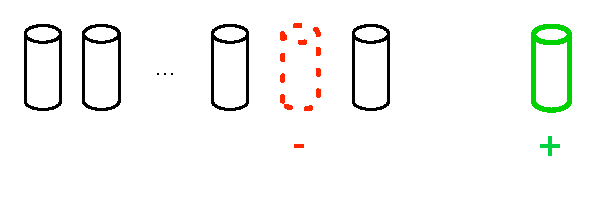
\includegraphics[width=\textwidth]{fig/exchange-multi}
	\caption{An exchange set from $\B_{\Matroid(n)}$ (\MultiIdent: \Cref{fact:topk}; each cylinder represents an arm).}
	\label{fig:exchange:topk}	
\end{subfigure}
~
\begin{subfigure}[c]{0.45\textwidth}
	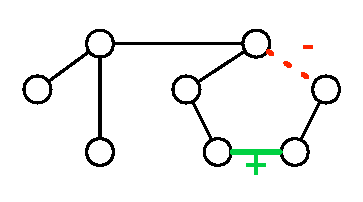
\includegraphics[width=\textwidth]{fig/exchange-matroid}
	\caption{An exchange set from $\B_{\Matroid(n)}$ (Spanning trees: \Cref{fact:matroid}; each edge corresponds to an arm).}
	\label{fig:exchange:matroid}
\end{subfigure}
~
\begin{subfigure}[c]{0.45\textwidth}
	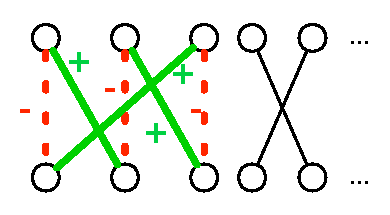
\includegraphics[width=\textwidth]{fig/exchange-match}
	\caption{An exchange set from $\B_{\Match(G)}$ (Matchings: \Cref{fact:match}; each edge corresponds to an arm) }
\end{subfigure}
~
\begin{subfigure}[c]{0.45\textwidth}
	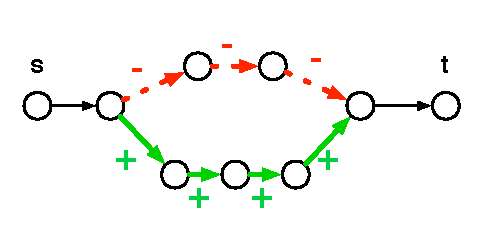
\includegraphics[width=\textwidth]{fig/exchange-path}
	\caption{An exchange set from $\B_{\Path(G,s,t)}$ (Paths: \Cref{fact:path}; each edge corresponds to an arm).}
\end{subfigure}
\caption{
Examples of exchange sets belonging to the exchange classes $\B_{\Matroid}$ (one for \MultiIdent and one for spanning tree), $\B_{\Match}$ and $\B_{\Path}$:
green-solid elements constitute the set $b_+$, red-dotted elements constitute the set $b_-$ and an example exchange set is given by $b=(b_+,b_-)$. 
In \Cref{fig:exchange:topk}, we use \MultiIdent as a specific instance of matroid decision class.
In \Cref{fig:exchange:matroid}, we use spanning tree as a specific instance of matroid decision class.
}
\label{fig:exchange}
\end{figure}


\begin{fact}[Matching]
\label{fact:match}
Let $G(V,E)$ be a bipartite graph with $n$ edges.
Let $\sigma\colon E\rightarrow [n]$ be a bijection.
Let $\mathcal A$ be the set of all valid matchings in $G$. 
We define $\M_{\Match(G)}$ as follows
$$
\M_{\Match(G)} = \big\{\sigma(A) \mid A\in\mathcal A \big\}.
$$
Define the exchange class
$$
\B_{\Match(G)} = \Big\{(\sigma(c_+),\sigma(c_-)) \mid \exists c\in \mathcal C\cup \mathcal P,\; \text{the edges of }c\text{ alternate between } c_+,c_-\Big\},
$$
where $\mathcal C$ is the set of all cycles in $G$ and $\mathcal P$ is the set of all paths in $G$.
Then we have $\B_{\Match(G)} \in \Exchange(\M_{\Match(G)})$. 
In addition, we have $\rank(\B_{\Match(G)}) \le |V|$, which implies that $\rank(\M_{\Matroid(T)}) \le |V|$. 
\end{fact}


To prove \Cref{fact:match}, we recall a classical result on graph matching which characterizes the properties of augmenting cycles and augmenting paths \citep{Berge15091957}.
\begin{lemma}
\label{lemma:match}
Let $G(V,E)$ be a bipartite graph.
Let $M$ and $M'$ be two different matching.
Then the induced graph $G'$ from the symmetric difference $(M\del M')\cup (M'\del M)$ consists of connected components that are one of the following
\begin{itemize}
%\item An isolated vertex.
\item An even cycle whose edges alternate between $M$ and $M'$.
\item A simple path whose edges alternate between $M$ and $M'$.
\end{itemize}
\end{lemma}




\begin{proof}[Proof of \Cref{fact:match}]
Fix  a bipartite graph $G(V,E)$ and a bijection $\sigma\colon E\rightarrow [n]$. 
Let $M,M' \in \M_{\Match(G)}$ be two different elements of $\M_{\Match(G)}$ and consider an arbitrary $e\in M\del M'$.
On a high level perspective, we construct an exchange class which contains all augmenting cycles and paths of $G$.
We know that the symmetric difference between $M$ and $M'$ can be decomposed into a collection of disjoint augmenting cycles and paths. 
And $e$ must be on one of the augmenting cycle or path. 
Then, since ``applying'' this augmenting cycle/path on $M$ will yield another valid matching which does not contains $e$. 
We see that this meets the requirements of an exchange class.
In the rest of the proof, we carry out the technical details of this argument.



Define $A=\sigma^{-1}(M)$ and $A'=\sigma^{-1}(M')$. 
Let $a=\sigma^{-1}(e)$.
Then $A,A'$ are two matchings of $G$. 
Let $G'$ be the induced graph from the symmetric difference $(A\del A')\cup(A'\del A)$.
Let $C$ be the connected component of $G'$ which contains the edge $a$.
Therefore, by \Cref{lemma:match}, we see that $C$ is either an even cycle or a  simple path with edges alternating between $A$ and $A'$.
Let $C_+$ contains the edges of $C$ that belongs to $A'\del A$.
Similarly, let $C_-$ contains the edges of $C$ that belongs to $A\del A'$.
Define $b_+ = \sigma(C_+)$ and $b_-=\sigma(C_-)$.
Let $b=(b_+,b_-)$ be an exchange set.

\junk{
Now we construct the exchange class.
Let $\mathcal C$ be the set of all cycles in $G$.
Let $\mathcal P$ be the set of all paths in $G$.
We define $\B_{\Match(G)}$ to correspond to the set of all cycles and all paths of $G$ with edges alternating between $b_+$ and $b_-$.
Formally, we have
$$
\B_{\Match(G)} = \Big\{(\sigma(c_+),\sigma(c_-)) \mid \exists c\in \mathcal C\cup P,\; \text{the edges of }c\text{ alternate between } c_+,c_-\Big\}.
$$
}

We see that $b\in \B_{\Match(G)}$.
Since $a\in C_-$, we obtain that $e\in b_-$.
In addition, note that $C_+ \subseteq A'\del A$ and $C_- \subseteq A\del A'$.
Therefore we have $b_+ \subseteq M'\del M$ and $b_- \subseteq M\del M'$.

%Consider the induced graph from $M \del C_- \cup C_+$.
Since $C$ is an $A$-augmenting path/cycle, therefore it immediately holds that $A\del C_-\cup C_+$ is a valid matching.
Therefore, we have $M\del b_- \cup b_+ \in \M_{\Match(G)}$.
Similarly, one can show that $M'\del b_+ \cup b_-\in \M_{\Match(G)}$.
Hence we have shown that $\B_{\Match(G)}$ is an exchange class for $\M_{\Match(G)}$.
%Observe that $\rank(\B_{\Match(G)}) \le |V|$. We conclude that $\rank(\M_{\Match(G)}) \le |V|$.
\end{proof}

\begin{fact}[Path]
\label{fact:path}
Let $G(V,E)$ be a directed acyclic graph with $n$ edges.
Let $s,t\in V$ be two different vertices.
Let $\sigma\colon E\rightarrow [n]$ be a bijection.
Let $\mathcal A(s,t)$ be the set of all valid paths from $s$ to $t$ in $G$. 
We define $\M_{\Path(G,s,t)}$ as follows
$$
\M_{\Path(G,s,t)} = \big\{\sigma(A) \mid A\in\mathcal A(s,t) \big\}.
$$
Define exchange class
$$
\B_{\Path(G)} = \{(\sigma^{-1}(p), \sigma^{-1}(q)) \mid p,q \text{ are the arcs of two disjoint paths of }G\text{ with same endpoints}\}.
$$
Then, we have $\B_{\Path(G)} \in \Exchange(\M_{\Path(G,s,t)})$. 
In addition, we have $\rank(\B_{\Path(G)}) \le |V|$ and therefore $\rank(\M_{\Path(G,s,t)}) \le |V|$.
\end{fact}

\begin{proof}
Fix  a directed acyclic graph $G(V,E)$ and a bijection $\sigma\colon E\rightarrow [n]$. 
Fix two vertices $s,t\in V$.

We prove that $\B_{\Path(G)}$ is an exchange class for $\M_{\Path(G,s,t)}$.
Let $M,M' \in \M_{\Path(G,s,t)}$ be two different sets. 
Then $\sigma^{-1}(M),\sigma^{-1}(M')$ are two sets of arcs correspond to two different paths from $s$ to $t$.
Let $P=(v_1,\ldots,v_{n_1}),P'=(v_1',\ldots,v_{n_2}')$ denote the two paths, respectively. 
Also denote $E(P) = \sigma^{-1}(M)$ and $E(P') = \sigma^{-1}(M')$.


Fix $e\in M\del M'$ and define $a=\sigma^{-1}(e)$.
Suppose that $a$ is an arc from $u$ to $v$.
Suppose $v_i=u$ and $v_{i+1} = v$.
Define $j_1 = \argmax_{j \le i, v_j\in P'} j$ and $j_2 = \argmin_{j \ge i+1, v_j \in P'} j$.
Let $v_{k_1}' = v_{j_1}$ and $v_{k_2}'= v_{j_2}$ be the corresponding indices in $P'$.
Then, we see that $Q_1=(v_{j_1},v_{j_1+1},\ldots,v_{j_2})$ and $Q_2= (v_{k_1}',v_{k_1+1}', \ldots,v_{k_2}')$ are two different paths from $v_{j_1}$ to $v_{j_2}$. 
Denote the sets of arcs of $Q_1$ and $Q_2$ as $E(Q_1)$ and $E(Q_2)$. 

Let $b=(b_+,b_-)$, where $b_+=\sigma(E(Q_2)), b_-=\sigma(E(Q_1))$. We see that $b \in \B_{\Path(G)}$.
It is clear that $a\in E(Q_1)$, $E(Q_1) \subseteq E(P) \del E(P')$ and $E(Q_2) \subseteq E(P') \del E(P)$. 
Therefore $e\in b_-$, $b_-\subseteq M\del M'$ and $b_+\subseteq M'\del M$.

Now it is easy to check that $E(P_1)\del E(Q_1) \cup E(Q_2)$ equals the set of arcs of path $(v_1,\ldots, v_{j_1}, v_{k_1+1}',\ldots, v_{k_2-1}', v_{j_2},\ldots, v_{n_1})$ (recall that $v_{j_1}=v_{k_1}'$ and $v_{j_2}=v_{k_2}'$).
This means that $E(P_1)\del E(Q_1)\cup E(Q_2) \in \mathcal A(s,t)$ and therefore $M\del b_-\cup b_+ \in \M_{\Path(G,s,t)}$.
Using a similar argument, one can show that $M'\del b_+\cup b_- \in \M_{\Path(G,s,t)}$ and hence we have verified that 
$\B_{\Path(G)}\in\Exchange(\M_{\Path(G,s,t)})$.
%Hence we can conclude by observing that $\rank(\B_\Path(G)) \le |V|$.
\end{proof}



\junk{
\begin{fact} 
Let $\M\subseteq 2^{[n]}$ be one of our example types of decision classes. 
Then we can construct the exchange class for $\M$ and upper bound $\rank(\M)$ as follows.
\begin{itemize}
\item Define $\B_{\Matroid(n)}=\big\{(\{i\},\{j\})\mid\forall i\in [n], j\in [n]\big\}$. If $\M=\M_{\Matroid(T,\sigma)}$, then we have $\B_{\Matroid(n)} \in \Exchange(\M)$ and $\rank(\M) \le 2$.	  
\item Define $\B_{\Match(G,\sigma)}=\big\{(C_+,C_-)\mid \sigma^{-1}(C_+\cup C_-) \text{ is a cycle of }G\big\}$. If $\M=\M_{\Match(G,\sigma)}$, then we have $\B_{\Match(G)} \in \Exchange(\M)$ and $\rank(\M) \le |V|$.	  
\item Define 
$\B_{\Path(G,\sigma)}=\big\{ (P_1, P_2)\mid\sigma^{-1}(P_1)\text{ and }\sigma^{-1}(P_2)\text{ are two disjoint paths of }G\text{ with same endpoints}\big\}$. 
If $\M=\M_{\Path(G,s,t,\sigma)}$, then we have $\B_{\Path(G,\sigma)} \in \Exchange(\M)$ and $\rank(\M) \le |V|$.	  
\end{itemize}
Moreover, since \Matroid encompasses both \MultiIdent and \MultiBandit types of decision classes, we see that $\rank(\M) \le 2$ for decision classes $\M$ of these types.
\label{lemma:example-exchange-class}
\end{fact}
}


\section{Equivalence between Constrained Oracles and Maximization Oracles}

In this section, we present a general method to implement constrained oracles using maximization oracles.
The idea of the reduction is simple: one can impose the negative constrains $B$ by setting the corresponding weights to be sufficiently small; and one can impose the positive constrains $A$ by setting the corresponding weights to very large.
The reduction method is shown in Algorithm~\ref{algo:reduction}.
The correctness of the reduction is proved in \Cref{fact:coracle}.
%We show that our reduction works efficiently for many decision classes which admit efficient maximization oracles, including the examples we examined in the last section.
Furthermore, it is trivial to reduce from maximization oracles to constrained oracles. 
Therefore, \Cref{fact:coracle} shows that maximization oracles are equivalent to constrained oracles up to a transformation on the weight vector. 


%The idea of the reduction is straightforward. 
%One can enforce the positive constraints by setting the corresponding weights to be sufficiently large.
%Then, one solves a maximization oracle for the decision class which is the restriction of $\M$ onto $[n]\del b$.


\begin{algorithm}[ht]
{
\small
\begin{algorithmic}[1]
\Require $\vec w\in \RR^n$, $A \subseteq [n]$, $B\subseteq [n]$; Maximization oracle $\Oracle: \RR^n \rightarrow \M$
\State $L_1\gets \nor{\vec w}_1$
\For{$i=1,\ldots,n$}
  \If{$i\in A$}
    \State $w_1(i) \gets 3L_1$
  \Else
    \State $w_1(i) \gets w(i)$
  \EndIf
\EndFor
\State $L_2 \gets \nor{\vec w_1}_1$
\For{$i=1,\ldots,n$}
  \If{$i\in B$}
    \State $w_2(i) \gets -3L_2$
  \Else
    \State $w_2(i) \gets w_1(i)$
  \EndIf
\EndFor
\State $M \gets \Oracle(\vec w_2)$
\If{$B\cap M = \emptyset$ and $A\subseteq M$}
  \State $\out=M$
\Else
  \State $\out=\bot$
\EndIf
\State{\textbf{return: } $\out$}
\end{algorithmic}
\caption{$\COracle(\vec w, A,B)$}
\label{algo:reduction}
}
\end{algorithm}


%It is easy to see that $\Oracle_{\tilde \M}$
\begin{lemma}
\label{fact:coracle}
Given $\M\subseteq 2^{[n]}$, $\vec w\in \RR^{n}$, $A \subseteq [n]$ and  $B\subseteq [n]$, suppose that $A\cap B=\emptyset$.
Then the output $\out$ of  Algorithm~\ref{algo:reduction} satisfies
$\out\in \argmax_{M\in \M, A\subseteq M, B\cap M=\emptyset}w(M)$
where we use the convention that the $\argmax$ of an empty set is $\bot$.
%Therefore $\out=\COracle(\vec w,a,b)$.
Therefore Algorithm~\ref{algo:reduction} is a valid constrained oracle.
\end{lemma}


\begin{proof}
Let $\vec w_1$ and $\vec w_2$ be defined as in Algoritm~\ref{algo:reduction}.
Let $M=\Oracle(\vec w_2)$.
Let $\M_{A,B} = \{M\in \M \mid A\subseteq M, B\cap M =\emptyset \}$ be the subset of $\M$ which satisfies the constraints.
If $\M_{A,B} = \emptyset$. 
Then it is clear $M$ cannot satisfy both of the constraints $A \subseteq M$ and $B \cap M =\emptyset$. 
Therefore Algorithm~\ref{algo:reduction} returns $\bot$ in this case.

In the rest of the proof, we assume that $\M_{A,B} \not=\emptyset$. 
Since $\M_{A,B}$ is non-empty, we can fix an arbitrary $M_0 \in \M_{A,B}$, which will be used later in the proof. 
We will also frequently use the fact that for all $\vec v\in \RR^{n}$ and all $S\subseteq[n]$, we have 
\begin{equation}
\label{eq:r62-0}
-\nor{\vec v}_1 \le v(S) \le \nor{\vec v}_1.
\end{equation}

First we claim that $B\cap M =\emptyset$.
Suppose that $B\cap M\not=\emptyset$. 
Then there exists $i\in B \cap M$ and we fix such an $i$.
Then we have
\begin{align}
	w_2(M) &= w_2(M\del \{i\})+w_2(i) \nonumber\\
				 &\le w_2(M \del B) + w_2(i) \label{eq:r62-1}\\
				 &= w_1(M\del B)+w_2(i) \label{eq:r62-2} \\
				 &\le L_2-3L_2 = -2L_2, \label{eq:r62-3}
\end{align}
where Eq.~\eqref{eq:r62-1} follows from the fact that $w_2(j) = -L_2 \le 0$ for all $j \in B \del \{i\}$;
Eq.~\eqref{eq:r62-2} holds since $\vec w_1$ and $\vec w_2$ coincide on all entries of $M\del B$;
and Eq.~\eqref{eq:r62-3} follows from the definition $L_2 = \nor{\vec w_1}_1$ and Eq.~\eqref{eq:r62-0}.

On the other hand, observing that $B\cap M_0=\emptyset$, we can bound $w_2(M_0)$ as follows
\begin{align*}
w_2(M_0) = w_1(M_0) \ge -L_2.
\end{align*}
Therefore we see that $w_2(M_0) \ge w_2(M)$.
However, this contradicts to the definition of $M$ since $M \in \argmax_{M'\in \M} w_2(M')$.
Therefore our claim $B\cap M = \emptyset$ is true.
By this claim and since $\vec w_2$ and $\vec w_1$ coincide on entries of $[n]\del B$, we have
\begin{equation}
\label{eq:rdc1}
w_2(M) = w_1(M).
\end{equation}

Next we claim that $A \subseteq M$. Suppose that $A\not\subseteq M$. 
Then we have
\begin{align}
	w_2(M) &= w_1(M) = w_1(M\cap A)+w_1(M\del A) \nonumber \\
				 &= 3|M\cap A| L_1 + w(M\del A) \label{eq:r62-4}\\
				 &\le (3|A|-3) L_1+L_1 \label{eq:r62-5}\\
				 &= (3|A|-2)L_1, \label{eq:r62-6}
\end{align}
where Eq.~\eqref{eq:r62-4} follows from the definition of $\vec w_1$;
and Eq.~\eqref{eq:r62-5} follows from the assumption that $A\not\subseteq M$ and therefore $|M\cap A| \le |A|-1$.

On the other hand, using the fact that $A\subseteq M_0$ (since $M_0\in \M_{A,B})$, we have
\begin{align}
w_2(M_0) &= w_1(M_0) = w_1(A)+w_1(M_0 \del A) \label{eq:r62-10}\\
	 		   &= 3|A| L_1+w(M_0\del A)\label{eq:r62-7}\\
	 		   &\ge 3|A| L_1-L_1\label{eq:r62-8}\\
	 		   &= (3|A|-1)L_1, \label{eq:r62-9} 	 		   
\end{align}
where Eq.~\eqref{eq:r62-10} follows from the fact that $M_0\cap B=\emptyset$ and $A\subseteq M_0$;
Eq.~\eqref{eq:r62-7} follows from the definition of $\vec w_1$, which ensures that $\vec w_1$ and $\vec w$ coincide on $M_0\del A$;
and Eq.~\eqref{eq:r62-8} follows from Eq.~\eqref{eq:r62-0}.

Therefore, by combining Eq.~\eqref{eq:r62-6} and Eq.~\eqref{eq:r62-9}, we see that $w_2(M_0) > w_2(M)$. 
Again this contradicts to the definition of $M$, which proves the claim.


Now we see that $M\in \M_{A,B}$. 
Therefore, we remain to verify that $w(M) = \max_{M'\in\M_{A,B}} w(M')$.
Suppose that there exists $M_1\in \M_{A,B}$ such that $w(M_1) > w(M)$.
Notice that $B\cap M_1=\emptyset$ and $A\subseteq M_1$, we have
$$
w_2(M_1) = w_1(M_1) = w_1(M_1\del A)+w_1(B) = w(M_1\del A)+3|A|L_1 = w(M_1)+3|A|L_1-w(A).
$$
Similarly, one can show that $w_2(M) = w(M)+3|A|L_1-w(A)$.
By combining with the assumption that $w(M_1) > w(M)$
we see that $w_2(M_1) > w_2(M)$, which contradicts to the definition of $M$. 
Hence we have verified that $w(M) = \max_{M'\in\M_{A,B}} w(M')$.
\end{proof}

\section{Preliminary Experiments: Minimal Spanning Tree}
In this section, we present some preliminary experimental results of our algorithms \Algorithm and \AlgorithmBud. 
We conduct experiments on a real-world dataset with decision classes corresponding to spanning trees.
We compare our algorithms with the uniform allocation benchmark \Uniform discussed in \Cref{section:uniform}.
The experiment results show that the proposed algorithms are considerably more sample efficient than the \Uniform algorithm, which agrees with our theoretical analysis.


%Our implementations of \Algorithm and \AlgorithmBud slightly differs from our descriptions in Algorithm~\ref{algo:pac} and Algorithm~\ref{algo:budget}. For \AlgorithmBud,  
\newcommand{\imgsize}{0.30}
\begin{figure}[htbp]
\centering
\begin{subfigure}[c]{\imgsize\textwidth}
	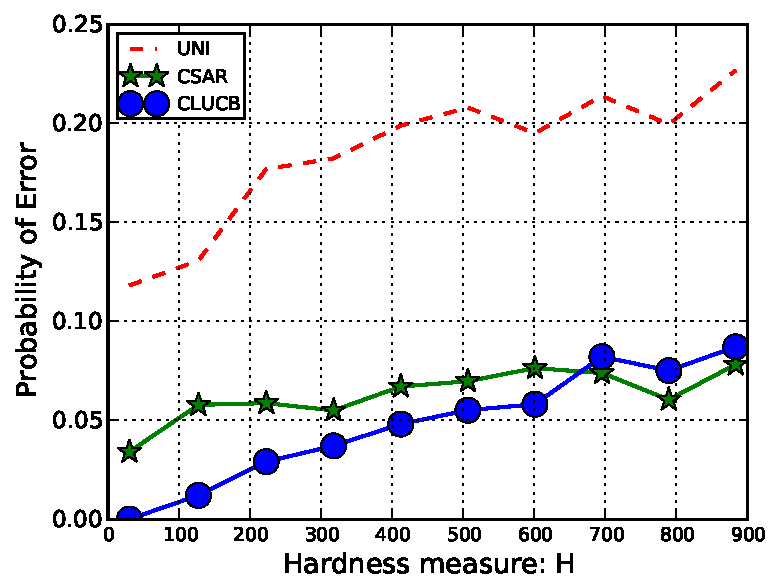
\includegraphics[width=\textwidth]{fig/exp/mst-c-1755}
	\caption{Network 1755}
\end{subfigure}
\begin{subfigure}[c]{\imgsize\textwidth}
	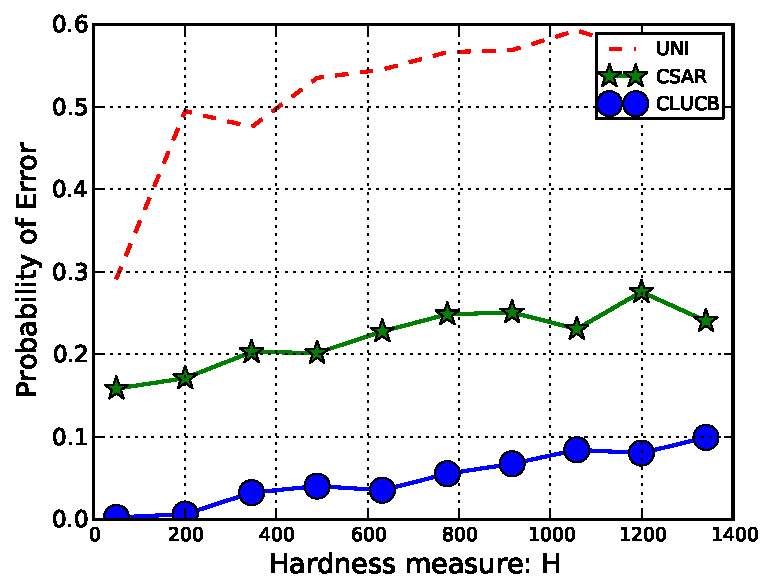
\includegraphics[width=\textwidth]{fig/exp/mst-c-3257}
	\caption{Network 3257}
\end{subfigure}
\begin{subfigure}[c]{\imgsize\textwidth}
	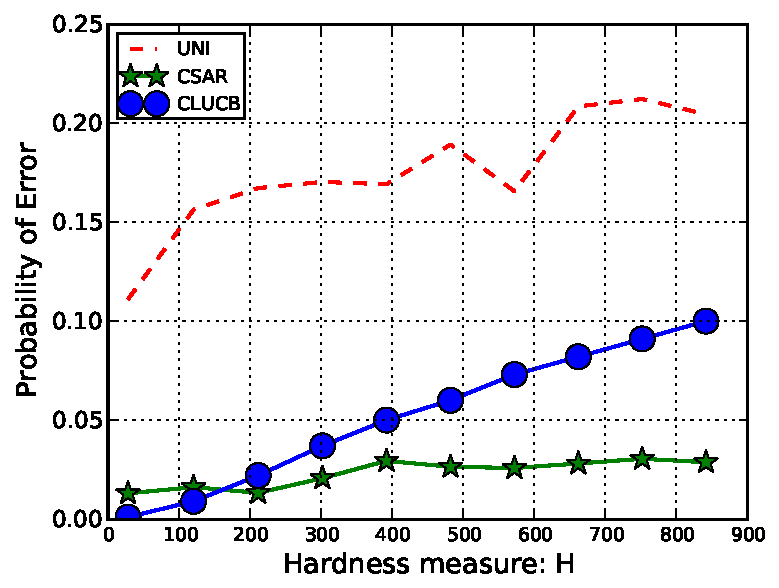
\includegraphics[width=\textwidth]{fig/exp/mst-c-3967}
	\caption{Network 3967}
\end{subfigure}
\caption{Comparison of empirical probability of errors  with respect to $\mathbf H$.}
\label{fig:exp1}
\end{figure}
\begin{figure}[htbp]
\centering
\begin{subfigure}[c]{\imgsize\textwidth}
	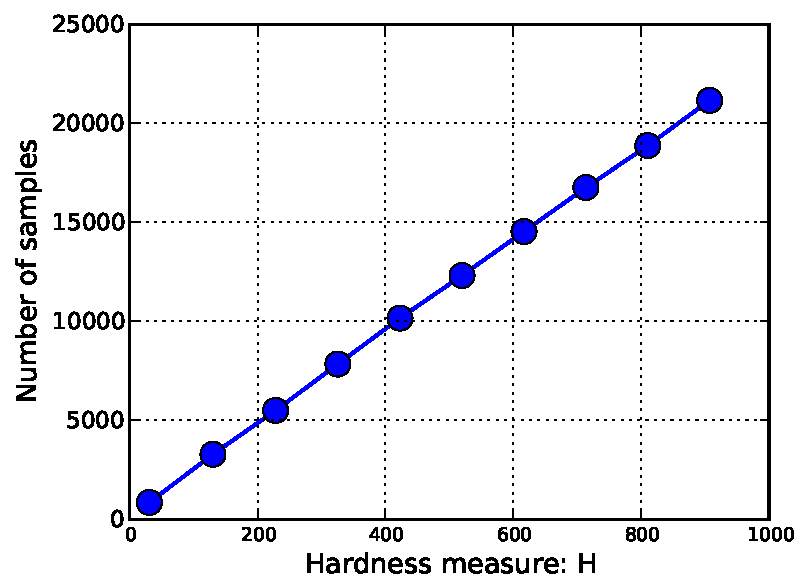
\includegraphics[width=\textwidth]{fig/exp/mst-cs-1755}
	\caption{Network 1755}
\end{subfigure}
\begin{subfigure}[c]{\imgsize\textwidth}
	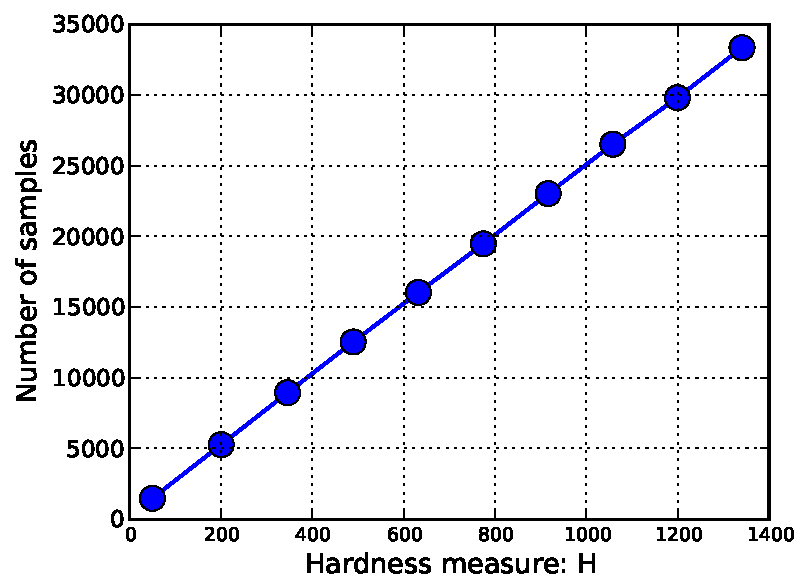
\includegraphics[width=\textwidth]{fig/exp/mst-cs-3257}
	\caption{Network 3257}
\end{subfigure}
\begin{subfigure}[c]{\imgsize\textwidth}
	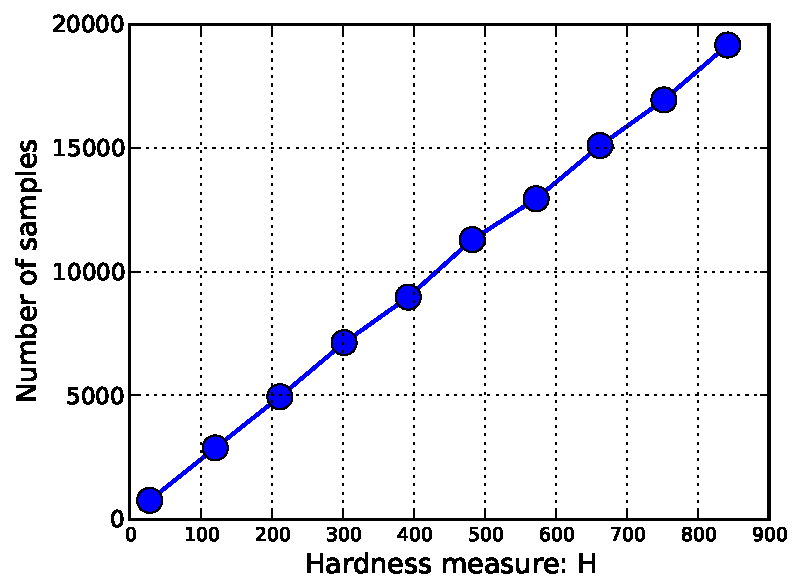
\includegraphics[width=\textwidth]{fig/exp/mst-cs-3967}
	\caption{Network 3967}
\end{subfigure}
\caption{Empirical sample complexity of \Algorithm with respect to $\mathbf H$.}
\label{fig:exp2}
\end{figure}
\begin{figure}[htbp]
\centering
\begin{subfigure}[c]{\imgsize\textwidth}
	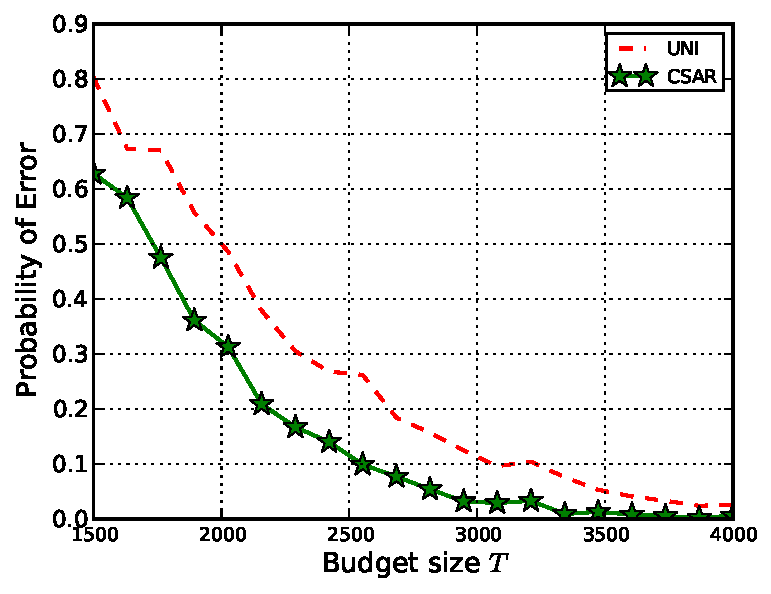
\includegraphics[width=\textwidth]{fig/exp/mst-1755}
	\caption{Network 1755}
\end{subfigure}
\begin{subfigure}[c]{\imgsize\textwidth}
	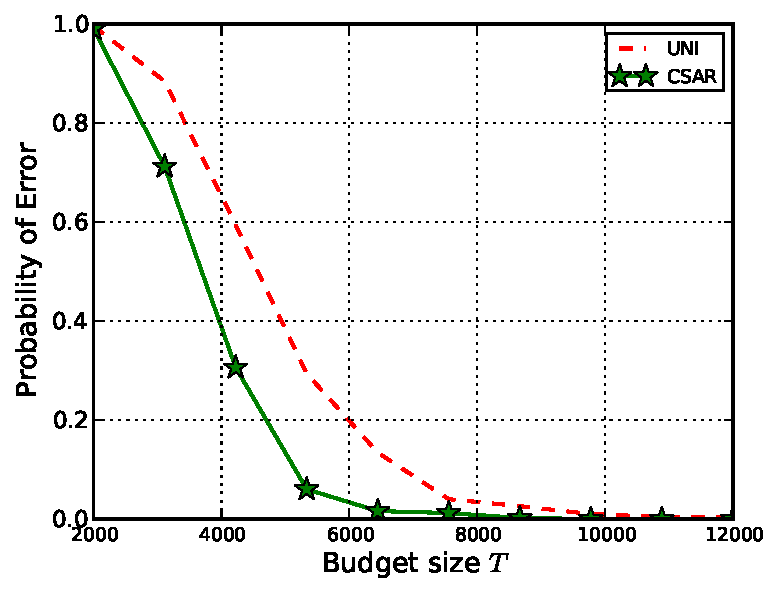
\includegraphics[width=\textwidth]{fig/exp/mst-3257}
	\caption{Network 3257}
\end{subfigure}
\begin{subfigure}[c]{\imgsize\textwidth}
	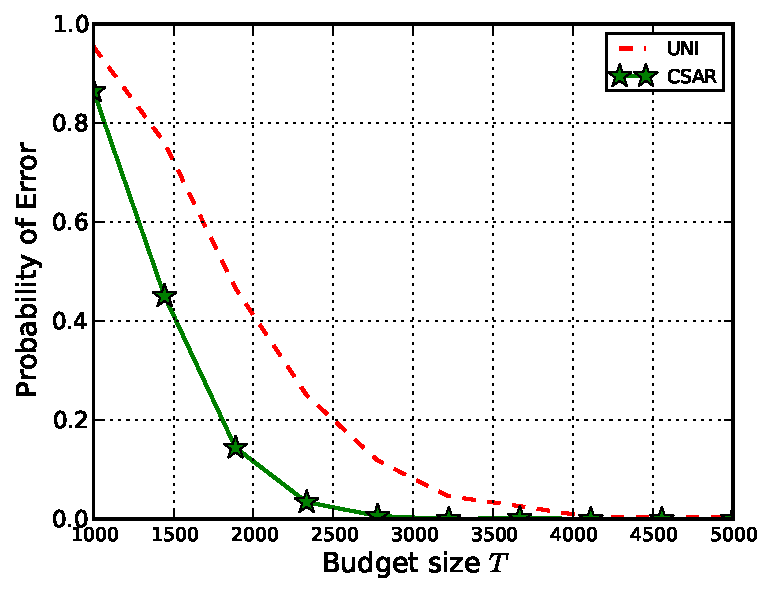
\includegraphics[width=\textwidth]{fig/exp/mst-3967}
	\caption{Network 3967}
\end{subfigure}
\caption{Empirical probability of error of \AlgorithmBud and \Uniform with respect to budget size $T$.}
\label{fig:exp3}
\end{figure}


\textbf{Setup.} 
Our task is to identify the optimal routing tree from a networking system, which has the lowest expected latency,  in an exploration procedure, in which one can obtain noisy measurements of latencies between different nodes.
We model this problem as a \Problem problem where the arms correspond to edges and the decision class corresponds to the set of spanning trees (which is a special case of matroids, as we have discussed in Example~\ref{example:matroid}).
We use a real-world dataset called RocketFuel \citep{spring2002measuring}, which contains several ISP networks with routing information such as average latencies between nodes pairs. 
We select three ISP networks with different numbers of edges ranging from $161$ to 328.
%The number of nodes 
%Among the six ISP networks, there are four fully connected networks which formed the dataset used in this experiment.
For each network, we model the latency $X(e)$ of edge $e$ as the sum of the given average latency $l(e)$ and an additive random noise $\mathcal N(0, 1)$.
Then we model the reward of edge $e$ as the negative latency $-X(e)$ and therefore the expected reward of $e$ is given by $w(e) = -l(e)$.
Notice that we now need to find the spanning tree that maximizes the expected reward, which is exactly an instance of \Problem. 

Since the ground-truth of expected reward $\vec w$ is known.
We can compute the ground-truth of the optimal set $M_*$ and the hardness measures $\mathbf H$.
Furthermore, in order to investigate the relationship between $\mathbf H$ and sample complexity empirically, we generate a number instances with different $\mathbf H$ by adjusting the expected reward of each arm $e\in M_*$ with a same amount $c_0$ while not changing the optimality of $M_*$.
By definition of $\mathbf H$, we see that $\mathbf H$ decreases when $c_0$ increases.
% and $\mathbf H$ increases if $c_0 < 0$.
%We will translate the sample complexity of \Algorithm in units of $\mathbf H$ in the spirit of the sample complexity bound of Theorem~\ref{theorem:main}.


\textbf{Evaluation method.} 
We use the following evaluation procedure to compare the sample efficiency between \Algorithm,\AlgorithmBud and \Uniform.
Since \AlgorithmBud and \Uniform are both learning algorithms in the fixed budget setting, the comparison between them is straightforward:
for each given budget, we run both algorithms with this budget independently for 1000 times and compare their empirical probability of errors (the fraction of runs where a tested algorithm fails to report the ground-truth optimal set $M_*$).
On the other hand, we use the following procedure to compare \Algorithm with other fixed budget algorithms.
We run \Algorithm independently for 1000 times with a given confidence parameter.
Suppose that the $i$-th run of \Algorithm uses $T_i$ samples, we also run \Uniform and \AlgorithmBud with budget $T_i$.
Then we compare the empirical probability of errors of the tested algorithms after the 1000 runs are completed.
In this way, we see the compared algorithms use an equal number of samples in each run, which allows us to compare their sample efficiency.
Finally, we set $\delta=0.3$ for \Algorithm throughout the experiments.
%In this way, we can compare the sample efficiency of \Algorithm with \Uniform and \AlgorithmBud.




\textbf{Experimental results.}
We test all competing algorithms using the aforementioned evaluation method.
The experimental results are shown in \Cref{fig:exp1}, \Cref{fig:exp2} and \Cref{fig:exp3}.
From the results (\Cref{fig:exp1} and \Cref{fig:exp3}), we see that both \Algorithm and \AlgorithmBud are consistently more sample efficient than \Uniform by a large margin, i.e. they incur a smaller empirical probability of error than \Uniform when using a same number of samples.
This matches our theoretical analyses of these algorithms.
We also see that the probability of error of \Algorithm is always smaller than the guarantee $\delta=0.3$ (Figure~\ref{fig:exp1}) and the sample complexity of \Algorithm is approximately linear in $\mathbf H$ (Figure~\ref{fig:exp2}), which agrees with our theory that the sample complexity bound for the spanning tree decision class is $\tilde O(\mathbf H)$ (see Example~\ref{example:matroid}).


%It is clear that the maximal spanning tree problem can be solved using a greedy algorithm.

%For each network used in this experiment, we identify the ground-truth optimal spanning tree using an offline algorithm. 
%We tune the hardness $\mathbf H$ by modifying the weights on the optimal spanning tree by a fixed amount.
%And for each different 
%Notice that our theory shows that a larger $\mathball H$ leads to a more difficult \Problem problem.




\bibliography{bandit}
\bibliographystyle{my-plainnat}
\end{document}
